% !TEX program = xelatex

\documentclass[12pt, a4paper]{article}

\usepackage{fontspec}
\setmainfont[Ligatures=TeX]{Linux Libertine O}
\usepackage[left=2.5cm,right=2.5cm,top=2.5cm,bottom=2.5cm]{geometry}
\usepackage{amsmath,amsfonts,amssymb}
\usepackage{dirtytalk}
\usepackage{bookmark}
\usepackage{cite}
\usepackage{graphicx}
\usepackage{subcaption}
\usepackage{float}
\usepackage{siunitx}
\usepackage{color}
\usepackage{indentfirst}
\usepackage{cleveref}
\usepackage{booktabs}
\usepackage{tabularx}

\graphicspath{{assets/}}

\sloppy


\begin{document}

\begin{titlepage}
    \begin{figure}[H]
      \begin{center}
        
\includegraphics[width=3cm]{auth.pdf}
        \label{fig:cover_auth_logo}
      \end{center}
    \end{figure}
    
    \centering
    \Large Αριστοτέλειο Πανεπιστήμιο Θεσσαλονίκης\\
    \Large Πολυτεχνική Σχολή\\
    \large Τμήμα Ηλεκτρολόγων Μηχανικών και Μηχανικών Υπολογιστών\\
    \large Τομέας Τηλεπικοινωνιών
    
    \vspace{\fill}
    
    \LARGE Multi-task learning in perturbation modeling
    
    \vspace{\fill}
    
    \Large Διπλωματική Εργασία\\
    \Large του\\
    \Large Θεόδωρου Κατζάλη
    
    \vspace{\fill}
    \raggedright
    
    \begin{tabular}{ll}
    \textbf{Επιβλέπων:} & Όνομα Επίθετο\\
     & Καθηγητής Α.Π.Θ.\\
    \end{tabular}
    
    \centering
    \vspace{\fill}
    \today
    
    \end{titlepage}
    
    % \begin{abstract}
    % abstract
    % \end{abstract}
    
    % \begin{abstract}
    % abstract
    % \end{abstract}
    
    % \thispagestyle{empty}
    
    
    % \section*{Ευχαριστίες}
    % \thispagestyle{empty}
    
    
    
    \clearpage
    

% \title{Τίτλος διπλωματικής}
% \author{Όνομα Επίθετο \\
% \href{mailto:empty@auth.gr}{empty@auth.gr}}
% \maketitle

{
\renewcommand*\contentsname{Περιεχόμενα}
\hypersetup{linkcolor=black}
\tableofcontents
}

\thispagestyle{empty}

\clearpage

\section{Abstract}

With the recent advancements in single-cell technology and the large scale perturbation datasets, the field of perturbation modeling  has created an opportunity for a wide variety of computational methods to be leveraged to harness its potential. Multi-task learning is one of the methods that has been left unexplored in this field. In this study we aim to bridge this gap unraveling the potential of multi-task learning in single-cell perturbation modeling.

% I have mentioned that scvidr is a multi-task model. Thus, maybe I have to rephrase it since there were some attempts but not fully dedicated to explore the multi-task as a learning paradigm per se.

\section{Introduction}    

The complexity of biological systems have imposed a challenge to capture the underlying mechanisms of cellular heterogeneity. Deciphering the effect of external stimuli (perturbation) at the cellular level, a field referred to as perturbation modeling \cite{jiMachineLearningPerturbational2021}, 
%has a significant impact
plays a crucial role
in biomedicine and drug discovery. With the recent surge of data 
generation, machine learning methods aim to understand the effect of perturbations and to extrapolate on unseen events.

An overview of the models on perturbation modeling can be found on this study \cite{gavriilidisMinireviewPerturbationModelling2024}. One of the main objectives is the out-of-distribution detection, which is the focal point of our study. The task is about predicting the perturbation response of the omics signature of cells with a specific cell type, while having observed the perturbation response of other cell types.

UnitedNet \cite{tangExplainableMultitaskLearning2023} is a multi-task framework that has shown its potential in multi-omics tasks such as cross modal prediction and cell type classification. We aim to extend this approach to perturbation modeling.


\section{Current single-cell perturbation modeling methods}

In the literature body, there are several approaches for predicting single-cell perturbation responses. To compare our multi-task method, we have chosen the models of scGen \cite{lotfollahiScGenPredictsSinglecell2019}, scPreGAN \cite{weiScPreGANDeepGenerative2022}, scButterfly \cite{caoScButterflyVersatileSinglecell2024}, and scVIDR \cite{kanaGenerativeModelingSinglecell2023}.

scGen projects the gene expression profile to a probabilistic latent space with a VAE. Then, the perturbation effect is modeled with a vector that represents the difference between the control and perturbed gene expression projections in the latent space.

scVIDR builds upon scGen by enhancing the architecture with cell type–specific knowledge. It is capable of predicting cellular responses to multiple chemical perturbations in a dose-dependent manner. As a multi-task model, scVIDR leverages data from various perturbations to improve prediction accuracy across conditions.

scPreGAN is based on a GAN and autoencoder setup. The study aims to decouple the perturbation effect from the latent space, and to apply it to the decoder stage.
%This approach could be explored in a multi-task multi-head architecture, where each head will be responsible for a specific perturbationm given a perturbed decoupled latent space. 

scButterfly was not originally designed for perturbation modeling. However, its cross-modal architecture, which includes dual aligned VAEs, can be repurposed for perturbation tasks. Rather than predicting one omic modality from another, the model can treat perturbed and control gene expression profiles as distinct modalities.

The performance of all of these models will serve as a baseline of our multi-task learning architecture.


\section{Method}

Multi-task learning is a machine learning paradigm and its core idea is that training a model to solve multiple tasks can be more effective than training separate models for each specific task \cite{zhangSurveyMultiTaskLearning2021}. A joint architecture that shares knowledge between the tasks can lead to better generalization.
The relationship of the tasks determines the positive or negative transfer to each other and the overall effectiveness of the paradigm.

Defining as a task the prediction of the gene expression given a perturbation, we will explore designing a model that can predict gene expressions after a perturbation for a set of perturbations.

One of the key problems of deep learning methods is the data demand. Another benefit of multi-task learning is the combination of data from multiple sources of informations, especially in perturbation modeling where the data is limited for a specific number of perturbations. 

To integrate the tasks, we have explored the application of feature-wise transformations \cite{dumoulin2018feature-wise}. For this kind of transformation, we have:

\[ \text{FiLM(x)} = \gamma (z) \odot x + \beta (z) \]

, where $\gamma$, and $\beta$ are learnable parameters generated by a network that represent a condition $z$ (e.g. a vector that indicates the task), and $x$ is the input.

This particular technique is referred to as conditional affine transformation (a combination of multiplicative and additive conditioning) that shifts and scales the input element-wise. It is efficient in terms of scaling and parameters compared to multi-head architectures, where each task has its dedicated network to generate the output of the task.


\begin{figure}
    \centering
    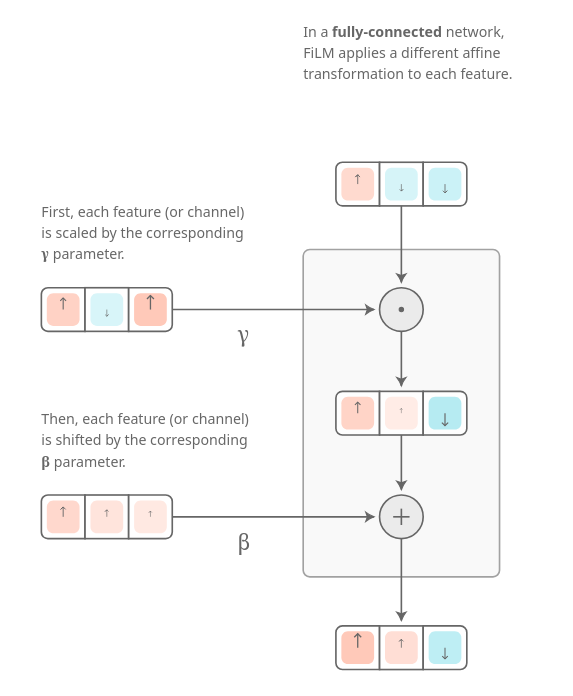
\includegraphics[width=0.5\textwidth]{film_layers.png}
    \caption{Illustration of the feature-wise transformation \cite{dumoulin2018feature-wise}}
    \label{fig:film}
\end{figure}

In our approach, we aim to decouple the perturbation effect by constructing a perturbation-free latent space, while explicitly modeling the perturbation response through a conditioning vector. Our architecture is built around an autoencoder, where task-specific conditioning — in our case, the type of perturbation — is integrated via FiLM layers fused into the decoder (\verb|MTAe|). The modulation parameters $\gamma$ and $\beta$ are learned independently for each fusion point.

The loss is the reconstruction loss of the autoencoder, which is the mean squared error between the input and the output of the decoder:

\[
\mathcal{L}_{\text{recon}} = \frac{1}{N} \sum_{i=1}^{N} ||x_i - \hat{x}_i||^2 \]


, where $x_i$ is the input gene expression profile, $\hat{x}_i$ is the reconstructed gene expression profile, and $N$ is the number of samples.

Regarding data splitting, we hold of the stimulated samples of the cell type of interest as a test set. The controlled ones, along with the rest of the cell types in both conditions of control and stimulated, are used for training. Thus, the autoencoder during training attempts to reconstruct the gene expressions while the condition vector is set accordingly to the type of perturbation. The condition vector is one-hot encoded, and given a dataset with N perturbations, its length is N+1, including the control condition.

\begin{figure}
    \centering
    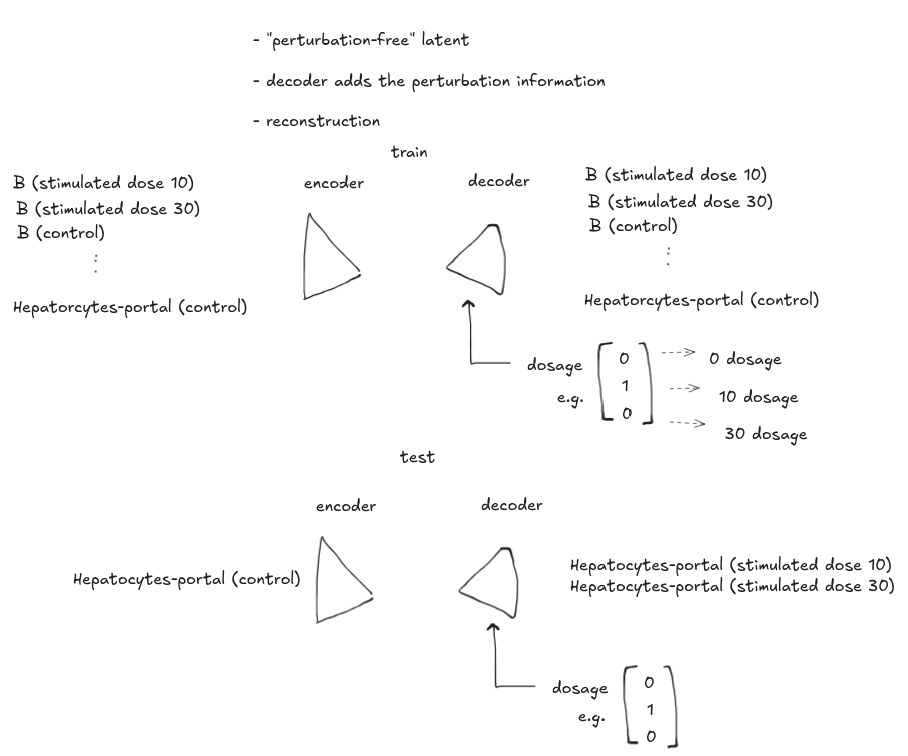
\includegraphics[width=0.7\textwidth]{ae_sketch.png}
    \caption{Illustration of the multi-task architecture. The encoder is shared across all tasks, while the decoder is conditioned by the task-specific FiLM layers.}
\end{figure}
% I have to document the losses

We have explored several variations of this approach, all of which maintain the decoder architecture with the inclusion of FiLM-based conditioning. These variations can be split to three main groups, a) adversarial autoencoders, b) optimal transport, c) Variational Autoencoders (VAEs).

Regarding the first ones, we are aiming to enforce a condition in the latent space via an adversarial loss. The architecture consists of the aforementioned autoencoder scheme with the FiLM layers with the addition of the discriminator. The discriminator aims to differentiate between samples of the latent space and a target distribution, while the encoder aims to fool the discriminator via an adversarial loss to enforce the target distribution in the latent space. For the  \verb|MTAeAdv| architecture, we have attempted to explicitly model a perturbation-free latent space, by using a discriminator to differentiate between the control and perturbed gene expression profiles. In that case, the samples were drawn from the latent space. Similarly, the \verb|MTAeAdv| architecture aims to enforce a Gaussian distribution in the latent space, by using a prior Gaussian distribution for the discriminator to sample from. 

\begin{figure}
    \centering
    \begin{subfigure}[t]{0.48\textwidth}
        \centering
        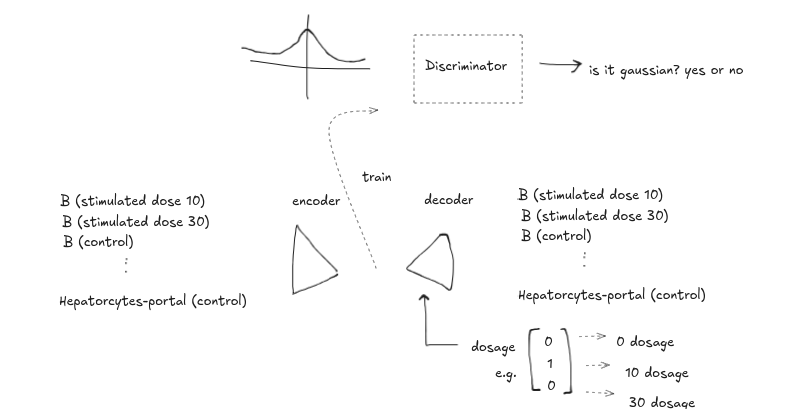
\includegraphics[width=\textwidth]{ae_gauss_sketch.png}
        \caption{}
        \label{}
    \end{subfigure}
    \hfill
    \begin{subfigure}[t]{0.48\textwidth}
        \centering
        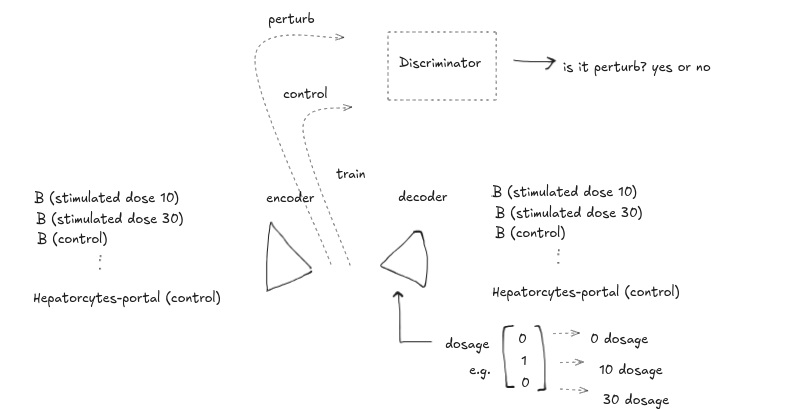
\includegraphics[width=\textwidth]{ae_adv_sketch.png}
        \caption{}
        \label{}
    \end{subfigure}
    \caption{Adversarial autoencoders}
    \label{}
\end{figure}

Another set of variations is the inclusion of optimal transport. In single-cell RNA sequencing, we can't sequence the same cell before and after a perturbation, thus we compare distributions since we lack the pair-wise information. To mitigate this, optimal transport can be used to create these pairs, by sampling from the perturbed distribution and matching it with the sample from the control distribution. Using that technique, instead of reconstructing the input, the goal was, given a sample from the controlled distribution, to predict its pair from the perturbed distribution. The loss is the mean squared error between the input and the output of the decoder, defined as:

\[
\mathcal{L}_{\text{OT}} = \frac{1}{N} \sum_{i=1}^{N} ||x_i - \hat{x}_i||^2 
\]

, where $x_i$ is the input gene expression profile, $\hat{x}_i$ is the pair from the perturbed gene expression profile, and $N$ is the number of samples. Compared to the previous architectures, the perturbed gene expression profiles are not fed in the network and used only to calculate the loss. This approach is named as \verb|MTAeOT|. Additionally, we have attempted to pretrain the model with the \verb|MTAe| architecture and then fine-tune it with the \verb|MTAeOT| architecture. This approach is named as \verb|MTAePlusOT|.

\begin{figure}
    \centering
    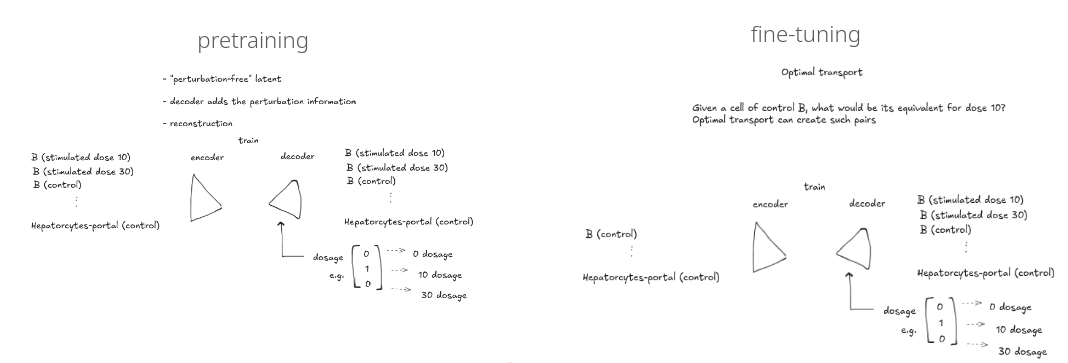
\includegraphics[width=\textwidth]{ae_ot_sketch.png}
    \caption{Using optimal transport to fine-tune the MTAe architecture (MTAePlusOT)}
\end{figure}

The last set of variations involves the inclusion of Variational Autoencoders (VAEs). The architecture builds upon the previously described autoencoder framework augmented with FiLM layers, while additionally incorporating a VAE loss to regularize the latent space. The VAE loss is defined as the sum of the reconstruction loss and the Kullback--Leibler (KL) divergence between the learned latent distribution and a standard normal prior:

\[
\mathcal{L}_{\text{VAE}} = \mathbb{E}_{q_\phi(z|x)}[\log p_\theta(x|z)] - D_{\text{KL}}(q_\phi(z|x) \,\|\, p(z))
\]

Here, $q_\phi(z|x)$ is the encoder's approximation of the posterior over latent variables, $p_\theta(x|z)$ is the decoder's likelihood of reconstructing the input, and $p(z) \sim \mathcal{N}(0, I)$ is the prior over latent variables. This model is named as \verb|MTVae|, and as we have described above with the optimal transport use case, we have the \verb|MTVaeOT| and \verb|MTVaePlusOT| architectures.

\begin{figure}
    \centering
    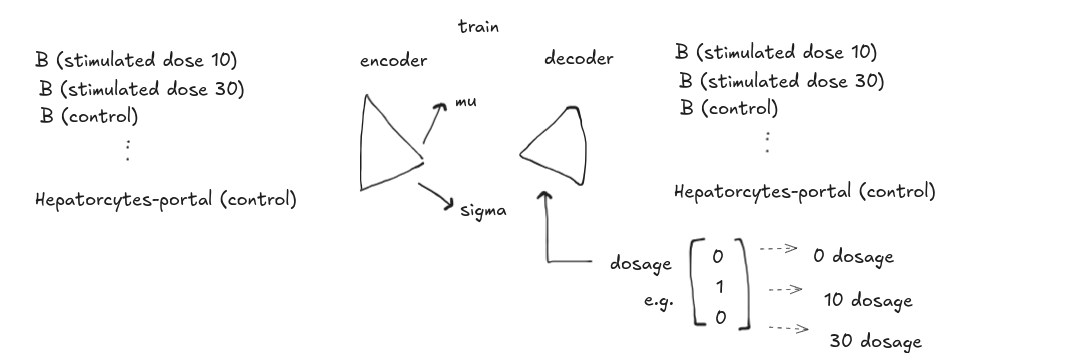
\includegraphics[width=0.8\textwidth]{vae_sketch.png}
    \caption{VAE}
\end{figure}


\section{Evaluation}

%Regarding data splitting, we hold of the stimulated samples of the cell type of interest as a test set. The controlled ones, along with the rest of the cell types in both conditions of control and stimulated, are used for training. The model is evaluated on the unseen cell type, given as input the control gene expression \cref{fig:umap_side_by_side}. The performance is measured by comparing the predicted gene expression with the actual one.

% explain the difference between single and multi, the hold off

We have tested the models on two datasets, one where human peripheral blood mononuclear cells have been stimulated by IFN-b interferon (Kang et al. \cite{kanaGenerativeModelingSinglecell2023}), and a multi-perturbation dataset, where liver cells have been stimulated by multiple doses of tetrachlorodibenzo-p-dioxin (TCDD) in vivo (Nault et al. \cite{nault2021single,nault2022benchmarking}).

The models are evaluated on the unseen cell type, given as input the control gene expression \cref{fig:umap_side_by_side}.
Regarding the single perturbation response models, the scGen, scButterfly, scPreGAN and scVIDR's single-task version, for the multi-perturbation dataset of ten dosages Nault et.al \cite{nault2021single,nault2022benchmarking}, we have trained a dedicated model for each dosage. In these cases, the dataset is consisted of only two conditions the control and the perturbed one for a particular dosage. The performance is measured by comparing the predicted gene expression with the actual one.

For this comparison, we have used the count of differentially expressed genes (DEGs), the $R^2$ of all the highly variable genes (HVGs), and the top 100 most variable ones. To complement the evaluation, we have calculated a set of five distance metrics (euclidean, edistance, wasserstein, mean pairwise, mmd) to capture the differences between the expected and predicted perturbed gene expressions in a point-wise and distributional manner using pertpy \cite{heumos2024pertpy}.

To address the randomness of the models, we have performed the experiments three times, with three different seeds 1, 2, 19193, and the metrics have been averaged across experiments.

To rank the models, since there could be conflicting cases between metrics, where one model could be better than the other, per model's metric we averaged them across all the experiments. Then we scaled them to the range of 0-1 with the following formula:

\[\frac{\text{current} - \text{best}}{\text{worst} - \text{best}}\]

% it could be reversed if highest is better

, that can track how a metric deviates from the best one. Then we summed all the metrics, giving a score (penalty) to each model. The model with the lowest score is considered the best one.

\begin{figure}[h!]
    \centering
    \begin{subfigure}[t]{0.48\textwidth}
        \centering
        \includegraphics[width=\textwidth]{figures/nault_umap_split_multiple.png}
        \caption{Nault et al. \cite{nault2021single,nault2022benchmarking}}
        \label{fig:nault_umap}
    \end{subfigure}
    \hfill
    \begin{subfigure}[t]{0.48\textwidth}
        \centering
        \includegraphics[width=\textwidth]{figures/pbmc_split.png}
        \caption{Kang et al. \cite{kanaGenerativeModelingSinglecell2023}}
        \label{fig:pbmc_umap}
    \end{subfigure}
    \begin{subfigure}[b]{0.48\textwidth}
        \centering
        \includegraphics[width=\textwidth]{figures/nault_umap_split_30.png}
        \caption{Example of single dose split of Nault et al. \cite{kanaGenerativeModelingSinglecell2023} for the dosage $30 \mu g/kg$}
        \label{fig:pbmc_umap}
    \end{subfigure}    
    \caption{UMAP representations of data split}
    \label{fig:umap_side_by_side}
\end{figure}

% \begin{figure}[h!]
%     \centering
%     \includegraphics[width=.7\textwidth]{figures/nault_umap_split_multiple.png}
%     \caption{Nault et al. \cite{nault2021single,nault2022benchmarking}}
%     \label{fig:nault_umap}
% \end{figure}

% \begin{figure}[h!]
%     \centering
%     \includegraphics[width=.7\textwidth]{figures/pbmc_split.png}
%     \caption{Kang et al. \cite{kanaGenerativeModelingSinglecell2023}}
%     \label{fig:pbmc_umap}
% \end{figure}


\section{Results}


% model & DEGs & $R^2_{\text{HVG}}$ & $R^2_{\text{HVG20}}$ & $R^2_{\text{HVG100}}$ & Euc & Was & E-dist & MPD & MMD \\


\begin{table}
    \centering
    \scalebox{0.8}{
    \begin{tabularx}{\textwidth}{lXXXXXXXXX}
    \toprule
    model & DEGs & $R^2_{\text{HVG}}$ & $R^2_{\text{HVG20}}$ & $R^2_{\text{HVG100}}$ & Euc & Was & E-dist & MPD & MMD \\
    \midrule
    MTAe & \textbf{0.000 (75.714)} & 0.077 (0.946) & 0.330 (0.871) & 0.140 (0.917) & 0.479 (0.488) & 0.815 (0.892) & 0.506 (0.651) & 0.898 (0.949) & 0.479 (0.488) \\
    MTAeAdv & 0.066 (72.381) & 0.026 (0.961) & 0.053 (0.955) & 0.043 (0.948) & 0.032 (0.202) & 0.006 (0.604) & 0.044 (0.429) & 0.110 (0.800) & 0.032 (0.202) \\
    MTAeAdvG & 0.195 (65.905) & 0.168 (0.917) & 0.305 (0.878) & 0.192 (0.901) & 0.503 (0.504) & 0.636 (0.828) & 0.570 (0.681) & 0.689 (0.909) & 0.503 (0.504) \\
    MTAeOT & 0.688 (41.190) & 1.000 (0.657) & 1.000 (0.668) & 1.000 (0.648) & 0.984 (0.811) & 0.969 (0.947) & 0.990 (0.883) & 0.976 (0.963) & 0.984 (0.811) \\
    MTAePlusOT & 0.768 (37.190) & 0.960 (0.670) & 0.983 (0.674) & 0.970 (0.657) & 0.982 (0.810) & 0.982 (0.951) & 0.983 (0.880) & 0.988 (0.966) & 0.982 (0.810) \\
    MTVae & 0.132 (69.095) & 0.088 (0.942) & 0.056 (0.954) & 0.105 (0.928) & 0.125 (0.261) & 0.056 (0.621) & 0.189 (0.499) & 0.114 (0.800) & 0.125 (0.261) \\
    MTVaeOT & 0.720 (39.571) & 0.961 (0.669) & 0.969 (0.678) & 0.953 (0.663) & 0.988 (0.813) & 0.993 (0.955) & 0.990 (0.883) & 0.992 (0.966) & 0.988 (0.813) \\
    MTVaePlusOT & 0.899 (30.619) & 0.987 (0.661) & 0.994 (0.670) & 0.976 (0.655) & 1.000 (0.821) & 1.000 (0.958) & 1.000 (0.888) & 1.000 (0.968) & 1.000 (0.821) \\
    scButterfly & 0.299 (60.727) & 0.251 (0.891) & 0.187 (0.914) & 0.232 (0.889) & 0.140 (0.271) & \textbf{0.000 (0.601)} & 0.128 (0.469) & \textbf{0.000 (0.779)} & 0.140 (0.271) \\
    scGen & 0.868 (32.143) & 0.191 (0.910) & 0.326 (0.872) & 0.290 (0.870) & 0.697 (0.627) & 0.863 (0.909) & 0.744 (0.765) & 0.885 (0.946) & 0.697 (0.627) \\
    scPreGAN & 0.796 (35.750) & 0.634 (0.771) & 0.376 (0.857) & 0.518 (0.799) & 0.496 (0.499) & 0.248 (0.690) & 0.572 (0.682) & 0.381 (0.851) & 0.496 (0.499) \\
    vidrSingle & 1.000 (25.536) & \textbf{0.000 (0.970)} & \textbf{0.000 (0.971)} & \textbf{0.000 (0.961)} & \textbf{0.000 (0.182)} & 0.014 (0.606) & \textbf{0.000 (0.408)} & 0.096 (0.797) & \textbf{0.000 (0.182)} \\
    \bottomrule
    \end{tabularx}}
    \caption{Score of the models for Kang et al. \cite{kanaGenerativeModelingSinglecell2023} along with the actual value in parenthesis}
\end{table}


\begin{table}
    \centering
    \scalebox{0.8}{
    \begin{tabularx}{\textwidth}{lXXXXXXXXX}
    \toprule
    model & DEGs & $R^2_{\text{HVG}}$ & $R^2_{\text{HVG20}}$ & $R^2_{\text{HVG100}}$ & Euc & Was & E-dist & MPD & MMD \\
    \midrule
    MTAe & \textbf{0.000 (20.341)} & 0.167 (0.862) & 0.267 (0.792) & 0.189 (0.833) & 0.056 (1.386) & 0.603 (1.217) & 0.116 (1.116) & 0.945 (1.050) & 0.056 (1.386) \\
    MTAeAdv & 0.368 (13.716) & 0.388 (0.792) & 0.518 (0.725) & 0.458 (0.743) & 0.025 (1.128) & 0.246 (1.091) & 0.045 (1.011) & 0.426 (1.017) & 0.025 (1.128) \\
    MTAeAdvG & 0.113 (18.307) & 0.339 (0.808) & 0.477 (0.736) & 0.396 (0.764) & 0.029 (1.164) & 0.293 (1.107) & 0.058 (1.030) & 0.607 (1.029) & 0.029 (1.164) \\
    MTAeOT & 0.650 (8.652) & 0.969 (0.608) & 0.829 (0.642) & 0.916 (0.590) & 0.001 (0.925) & 0.008 (1.006) & 0.005 (0.951) & 0.122 (0.998) & 0.001 (0.925) \\
    MTAePlusOT & 0.657 (8.519) & 0.956 (0.613) & 0.822 (0.644) & 0.897 (0.596) & \textbf{0.000 (0.917)} & \textbf{0.000 (1.004)} & 0.002 (0.948) & 0.099 (0.996) & 0.000 (0917) \\
    MTVae & 0.076 (18.981) & 0.339 (0.808) & 0.523 (0.724) & 0.428 (0.753) & 0.025 (1.124) & 0.273 (1.100) & 0.041 (1.005) & 0.413 (1.016) & 0.025 (1.124) \\
    MTVaeOT & 0.677 (8.163) & 0.953 (0.614) & 0.830 (0.642) & 0.906 (0.593) & 0.001 (0.929) & 0.016 (1.009) & 0.006 (0.952) & 0.132 (0.998) & 0.001 (0.929) \\
    MTVaePlusOT & 0.647 (8.701) & 0.948 (0.615) & 0.816 (0.645) & 0.894 (0.597) & 0.000 (0.919) & 0.008 (1.006) & 0.003 (0.948) & 0.112 (0.997) & \textbf{0.000 (0.919)} \\
    scButterfly & 0.196 (16.818) & 0.553 (0.740) & 0.633 (0.694) & 0.600 (0.696) & 0.008 (0.984) & 0.029 (1.014) & \textbf{0.000 (0.944)} & \textbf{0.000 (0.990)} & 0.008 (0.984) \\
    scGen & 0.781 (6.288) & \textbf{0.000 (0.915)} & \textbf{0.000 (0.863)} & \textbf{0.000 (0.897)} & 0.178 (2.408) & 0.637 (1.229) & 0.299 (1.387) & 0.805 (1.041) & 0.178 (2.408) \\
    scPreGAN & 0.324 (14.511) & 1.000 (0.599) & 1.000 (0.596) & 1.000 (0.562) & 0.007 (0.972) & 0.042 (1.019) & 0.017 (0.969) & 0.163 (1.000) & 0.007 (0.972) \\
    vidrMult & 1.000 (2.352) & 0.143 (0.870) & 0.099 (0.837) & 0.133 (0.852) & 1.000 (9.295) & 1.000 (1.358) & 1.000 (2.425) & 1.000 (1.054) & 1.000 (9.295) \\
    vidrSingle & 0.920 (3.795) & 0.191 (0.855) & 0.247 (0.797) & 0.216 (0.824) & 0.061 (1.431) & 0.480 (1.174) & 0.117 (1.118) & 0.544 (1.025) & 0.061 (1.431) \\
    \bottomrule
    \end{tabularx}}
    \caption{Score of the models for Nault et al. \cite{nault2021single,nault2022benchmarking} along with the actual value in parenthesis}
\end{table}


\begin{table}
    \centering
    \begin{tabular}{lrrr}
    \toprule
    model & score & baseline score & distance score \\
    \midrule
    MTAeAdv & 0.414099 & 0.188957 & 0.225142 \\
    MTVae & 0.989313 & 0.381226 & 0.608087 \\
    vidrSingle & 1.109933 & 1.000000 & 0.109933 \\
    scButterfly & 1.375249 & 0.968395 & 0.406855 \\
    MTAe & 3.723979 & 0.546259 & 3.177721 \\
    MTAeAdvG & 3.762873 & 0.860886 & 2.901987 \\
    scPreGAN & 4.519561 & 2.325642 & 2.193919 \\
    scGen & 5.559246 & 1.674543 & 3.884703 \\
    MTVaeOT & 8.552051 & 3.602547 & 4.949504 \\
    MTAeOT & 8.590746 & 3.688019 & 4.902727 \\
    MTAePlusOT & 8.598116 & 3.680466 & 4.917650 \\
    MTVaePlusOT & 8.855812 & 3.855812 & 5.000000 \\
    \bottomrule
    \end{tabular}
    \caption{Kang et al. \cite{kanaGenerativeModelingSinglecell2023}}
\end{table}
    
    
\begin{table}
    \centering
    \begin{tabular}{lrrr}
    \toprule
    model & score & baseline score & distance score \\
    \midrule
    scButterfly & 2.026767 & 1.981569 & 0.045198 \\
    MTVae & 2.142595 & 1.365570 & 0.777025 \\
    MTAeAdvG & 2.341641 & 1.324716 & 1.016925 \\
    MTAe & 2.398554 & 0.622043 & 1.776511 \\
    MTAeAdv & 2.498785 & 1.731406 & 0.767379 \\
    vidrSingle & 2.837696 & 1.573823 & 1.263873 \\
    scGen & 2.878990 & 0.781217 & 2.097772 \\
    MTVaePlusOT & 3.428329 & 3.305106 & 0.123224 \\
    MTAePlusOT & 3.433685 & 3.332175 & 0.101511 \\
    MTAeOT & 3.500992 & 3.363746 & 0.137247 \\
    MTVaeOT & 3.522593 & 3.365641 & 0.156953 \\
    scPreGAN & 3.559583 & 3.324068 & 0.235515 \\
    vidrMult & 6.375357 & 1.375357 & 5.000000 \\
    \bottomrule
    \end{tabular}
    \caption{Nault et al. \cite{nault2021single,nault2022benchmarking}}
\end{table}


\begin{figure}[h!]
    \centering
    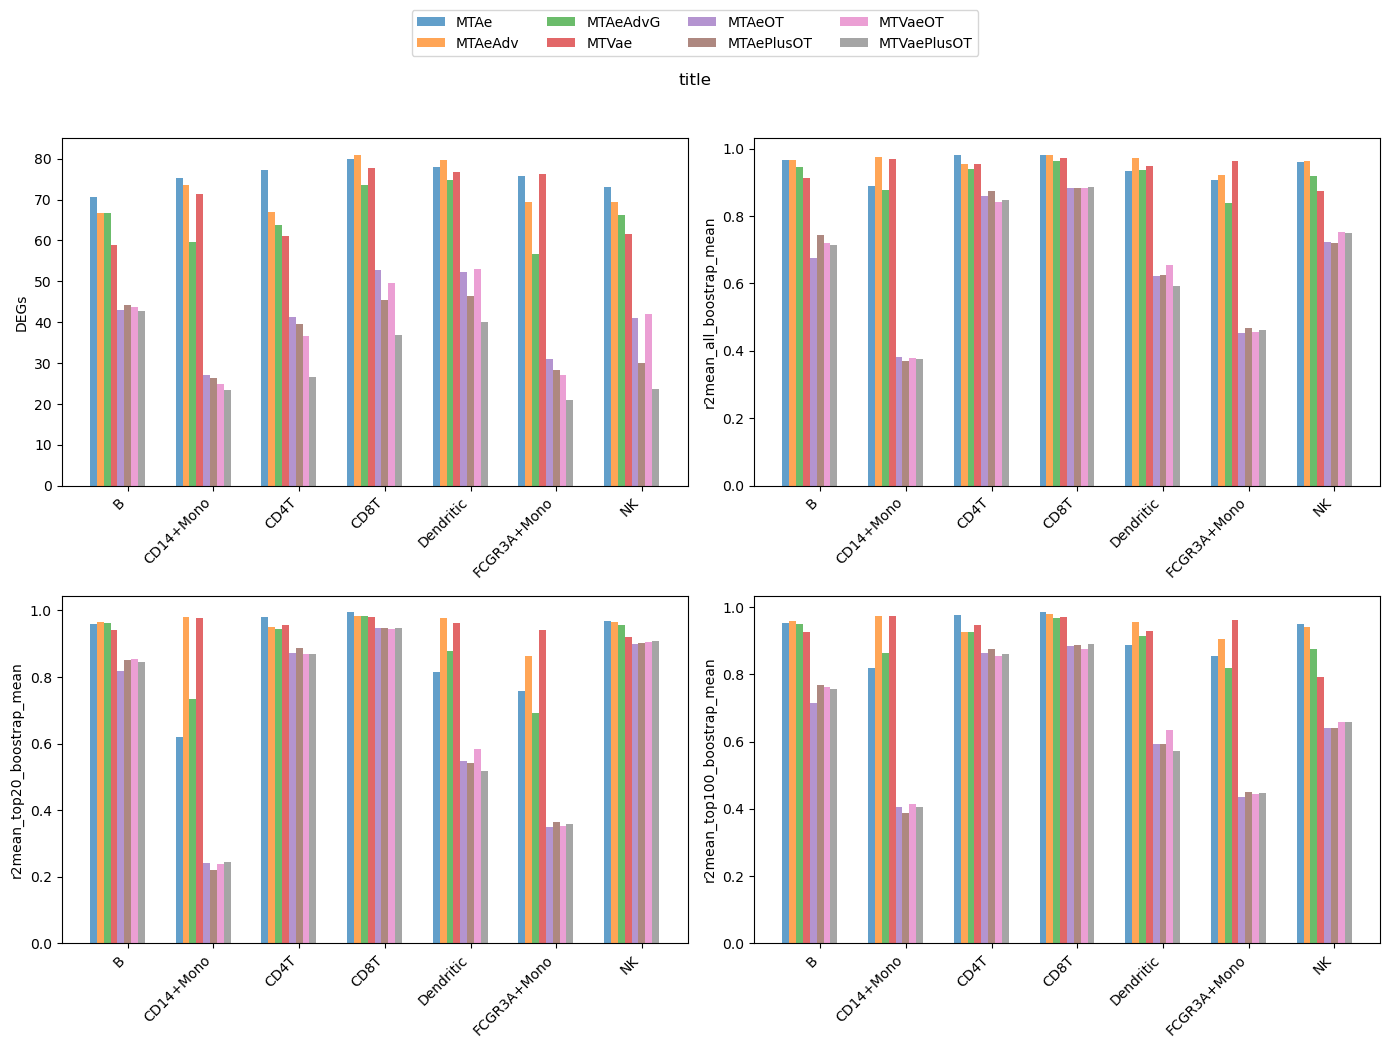
\includegraphics[width=.85\textwidth]{multi_task_benchmarking_cell_type_baseline_metrics_pbmc.png}
    \caption{Baseline metrics of multi-task models for the Kang et al. \cite{kanaGenerativeModelingSinglecell2023} dataset across cell types}
\end{figure}

\begin{figure}[h!]
    \centering
    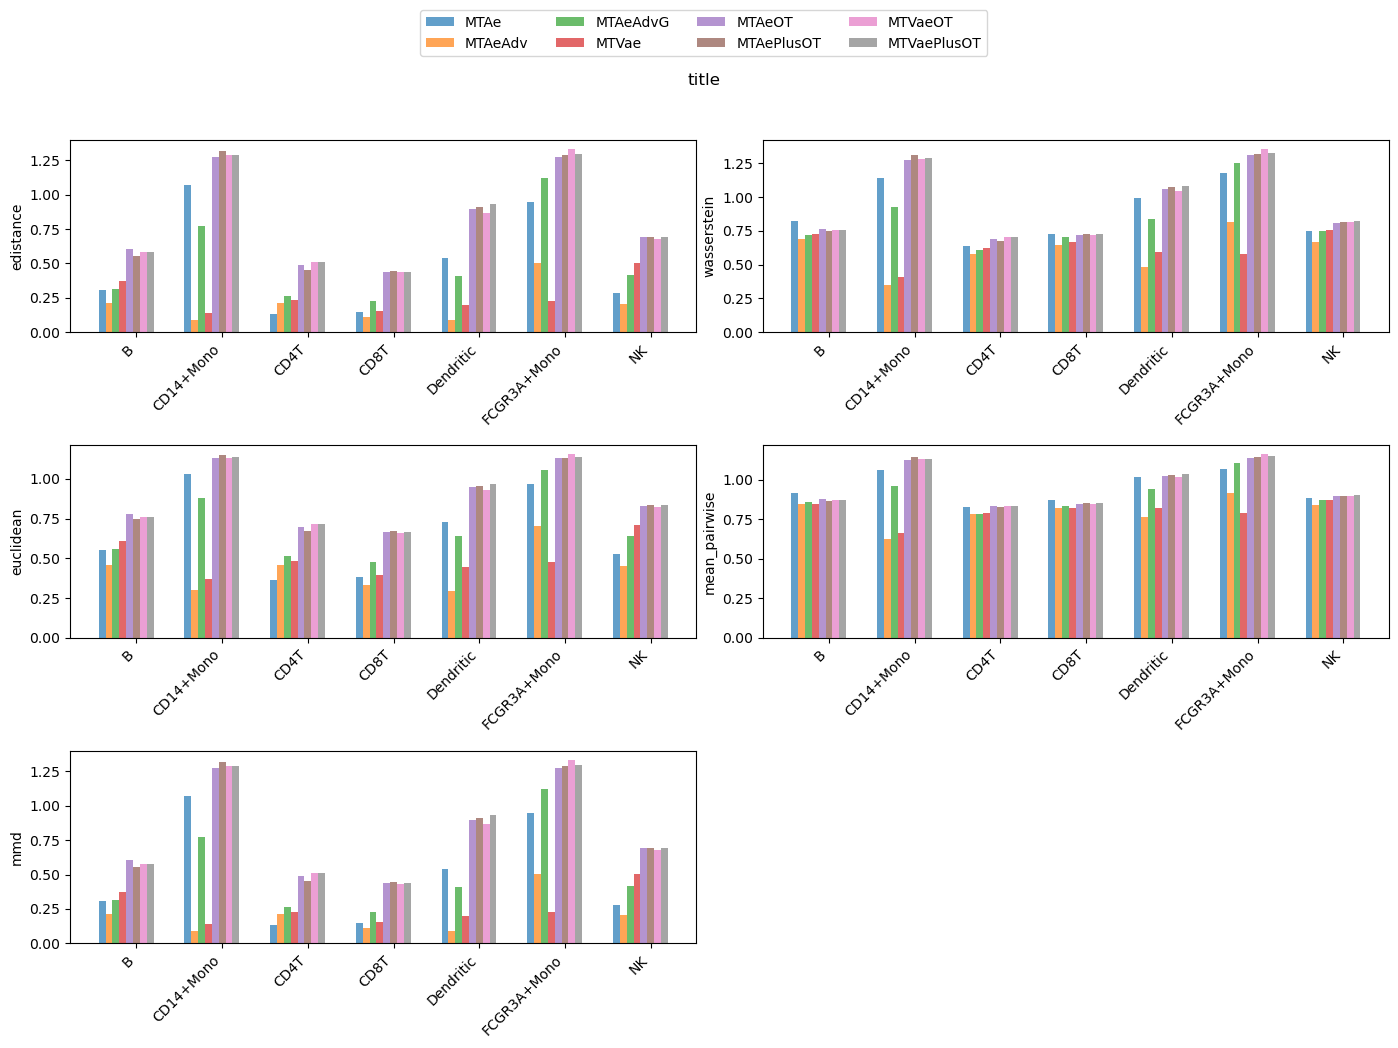
\includegraphics[width=.85\textwidth]{multi_task_benchmarking_cell_type_distance_metrics_pbmc.png}
    \caption{Distance metrics of multi-task models for the Kang et al. \cite{kanaGenerativeModelingSinglecell2023} dataset across cell types}
\end{figure}


\begin{figure}[h!]
    \centering
    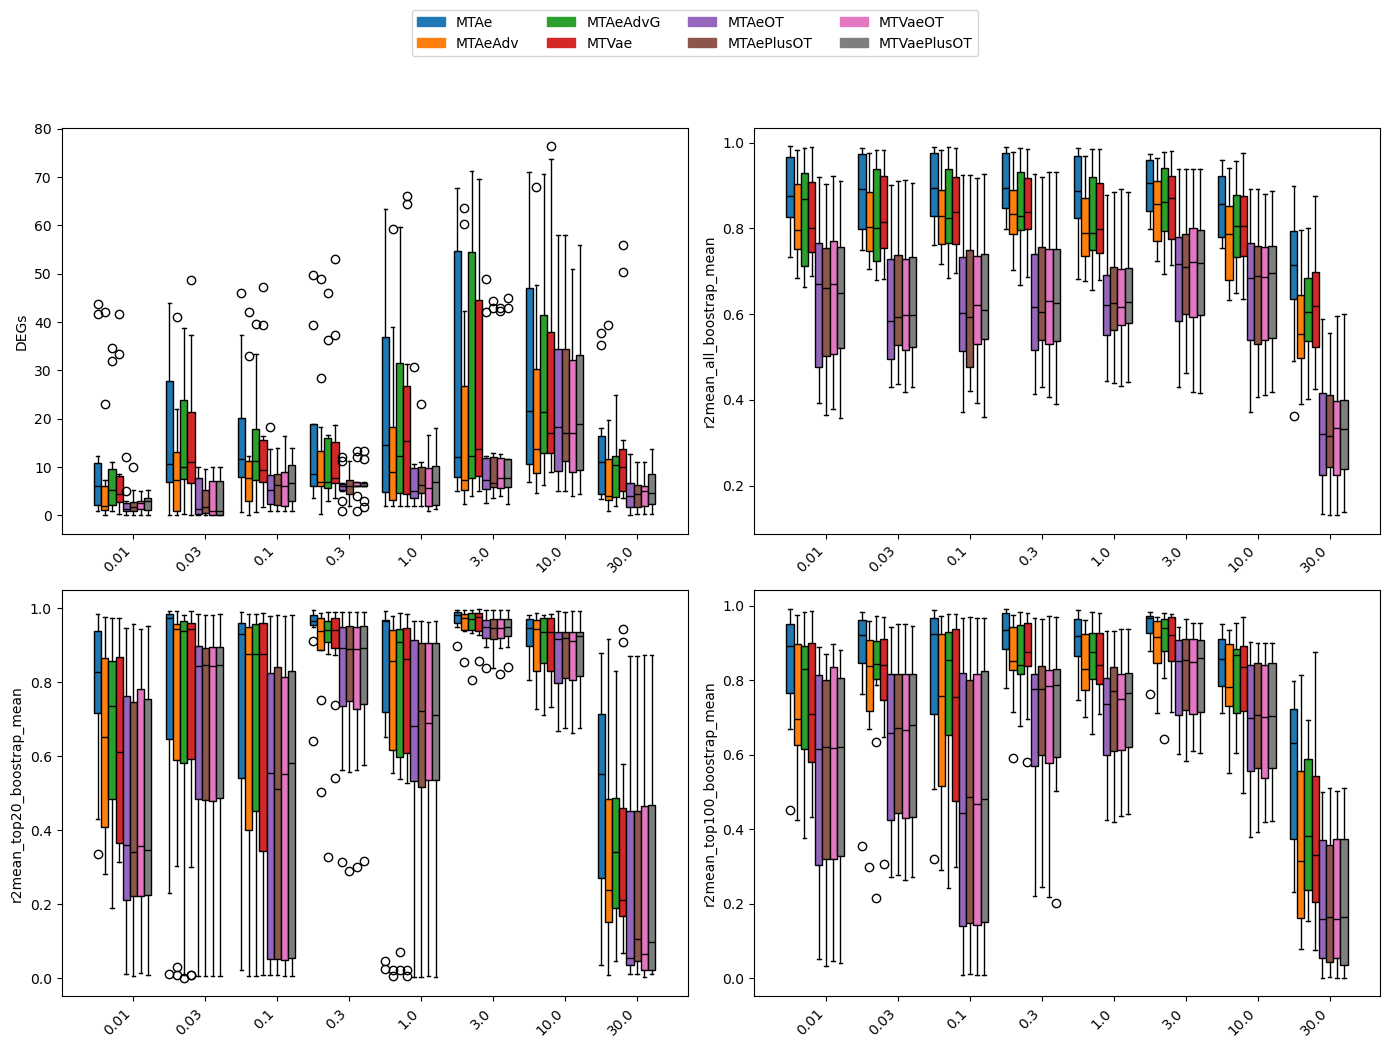
\includegraphics[width=.85\textwidth]{multi_task_benchmarking_doses_baseline_metrics_nault.png}
    \caption{Baseline metrics of multi-task models for the Nault et al. \cite{nault2021single,nault2022benchmarking} dataset across dosages}
\end{figure}

\begin{figure}[h!]
    \centering
    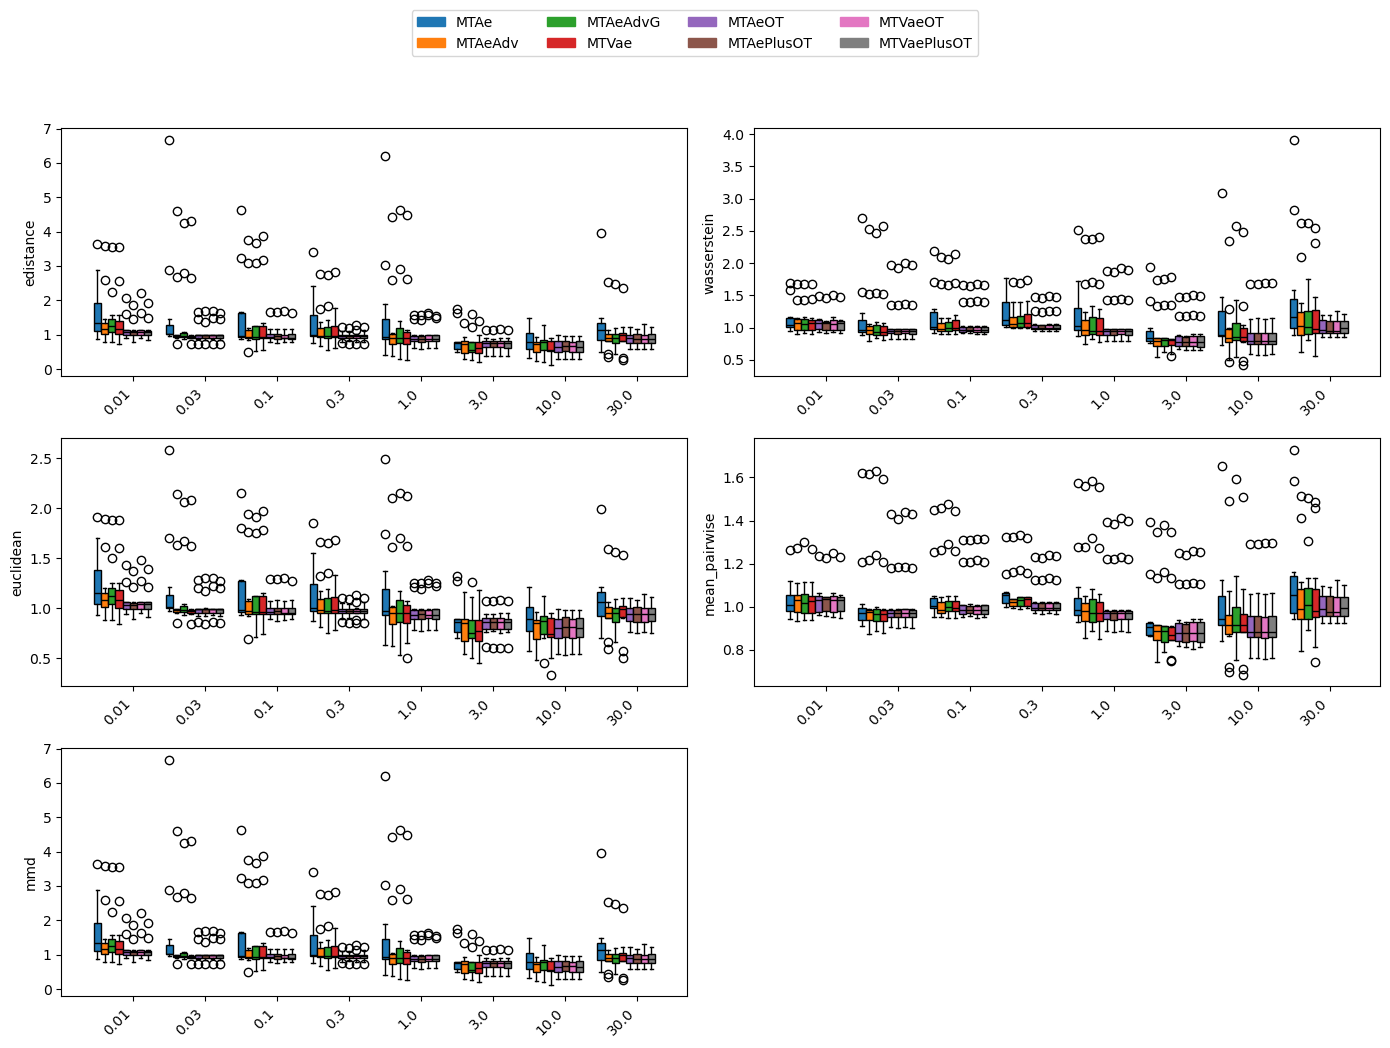
\includegraphics[width=.85\textwidth]{multi_task_benchmarking_doses_distance_metrics_nault.png}
    \caption{Distance metrics of multi-task models for the Nault et al. \cite{nault2021single,nault2022benchmarking} dataset across dosages}
\end{figure}


\begin{figure}[h!]
    \centering
    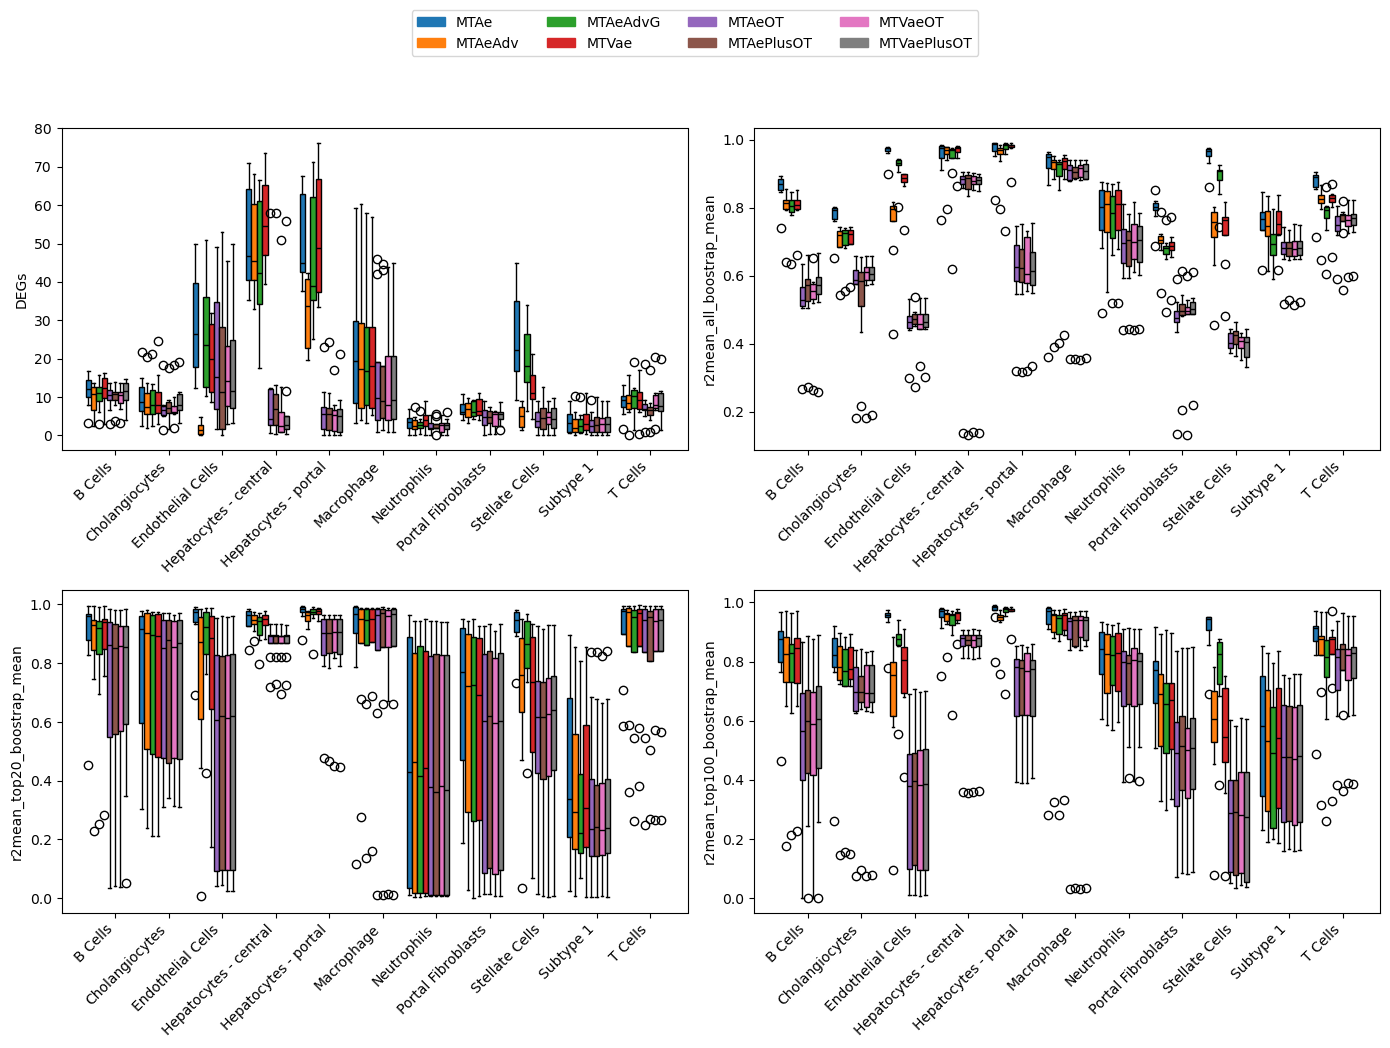
\includegraphics[width=.85\textwidth]{multi_task_benchmarking_cell_type_baseline_metrics_nault.png}
    \caption{Baseline metrics of multi-task models for the Nault et al. \cite{nault2021single,nault2022benchmarking} dataset across cell types}
\end{figure}


\begin{figure}[h!]
    \centering
    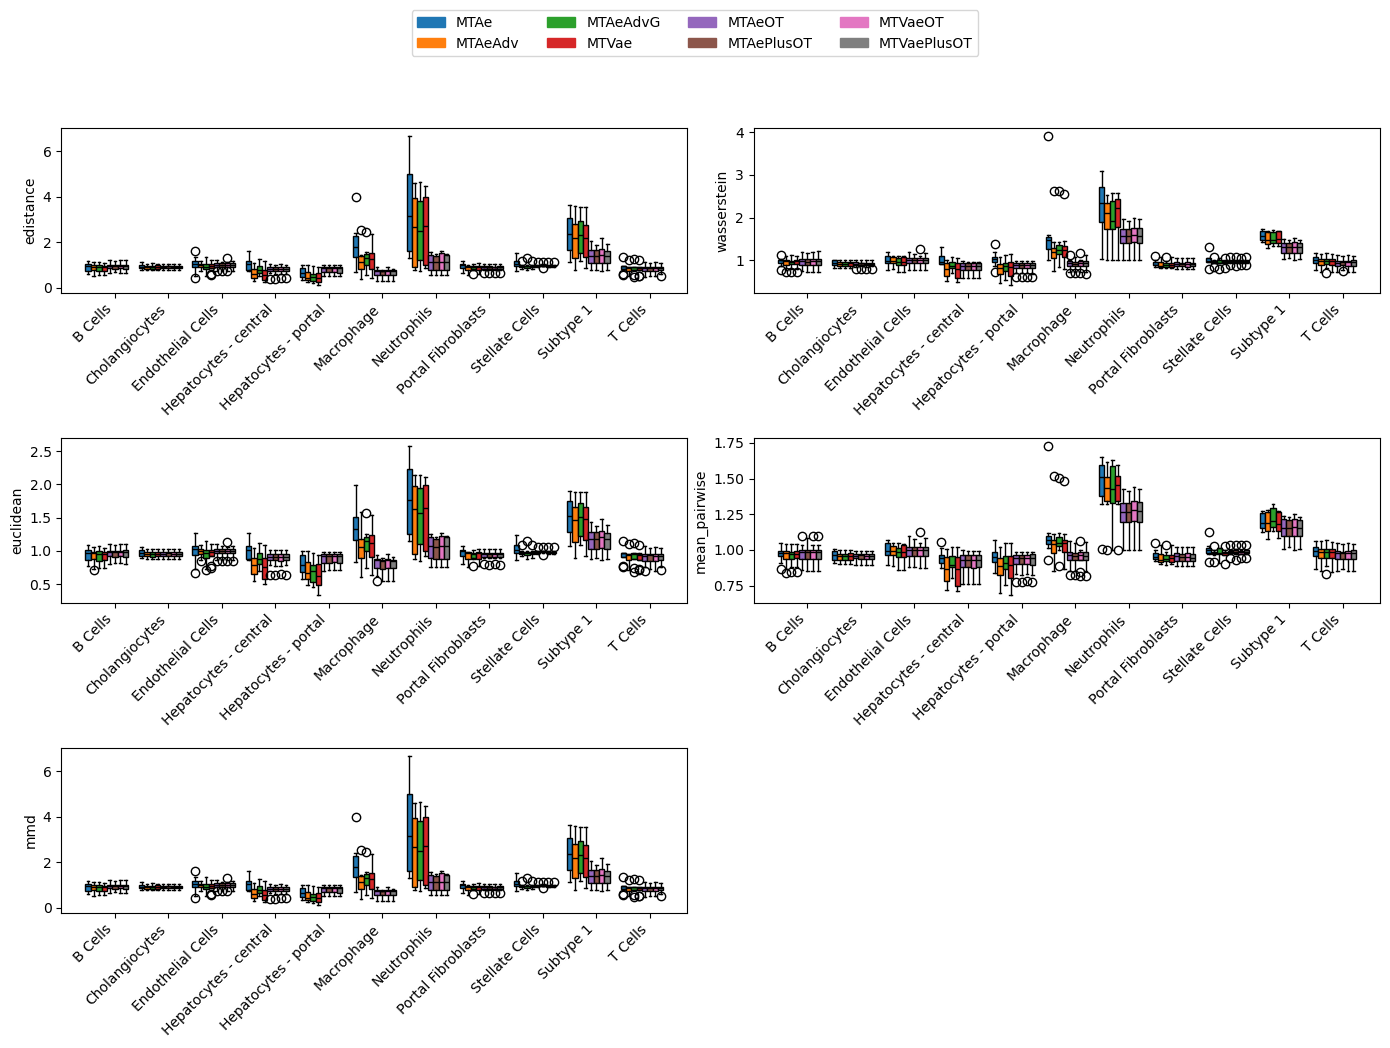
\includegraphics[width=.85\textwidth]{multi_task_benchmarking_cell_type_distance_metrics_nault.png}
    \caption{Distance metrics of multi-task models for the Nault et al. \cite{nault2021single,nault2022benchmarking} dataset across cell types}
\end{figure}


Initially, we will benchmark only our multi-task variations to filter out the most promising models \cref{fig:selected_pbmc_baseline,fig:selected_pbmc_distance,fig:selected_nault_cell_type_baseline,fig:selected_nault_cell_type_distance,fig:selected_nault_doses_baseline,fig:selected_nault_doses_distance}.
As we can see the best performing ones are MTAe, MTAeAdv, and MTAeAdvG. Thus, we will compare them with state-of-the-art literature models such as scButterfly, scVIDR, scPreGAN and scGen.

scVIDR performance drops for DEGs, and distance metrics, but it performs well for the $R^2$ metrics and stays very consistent, along with scGEN. The multi-task models and scButterfly exhibit greater variability across measurements, but better performance on average. The optimal transport variations performed poorly overall, but were among the best for distance metrics for the Nault et al. \cite{nault2021single,nault2022benchmarking} dataset. 

\begin{figure}[h!]
    \centering
    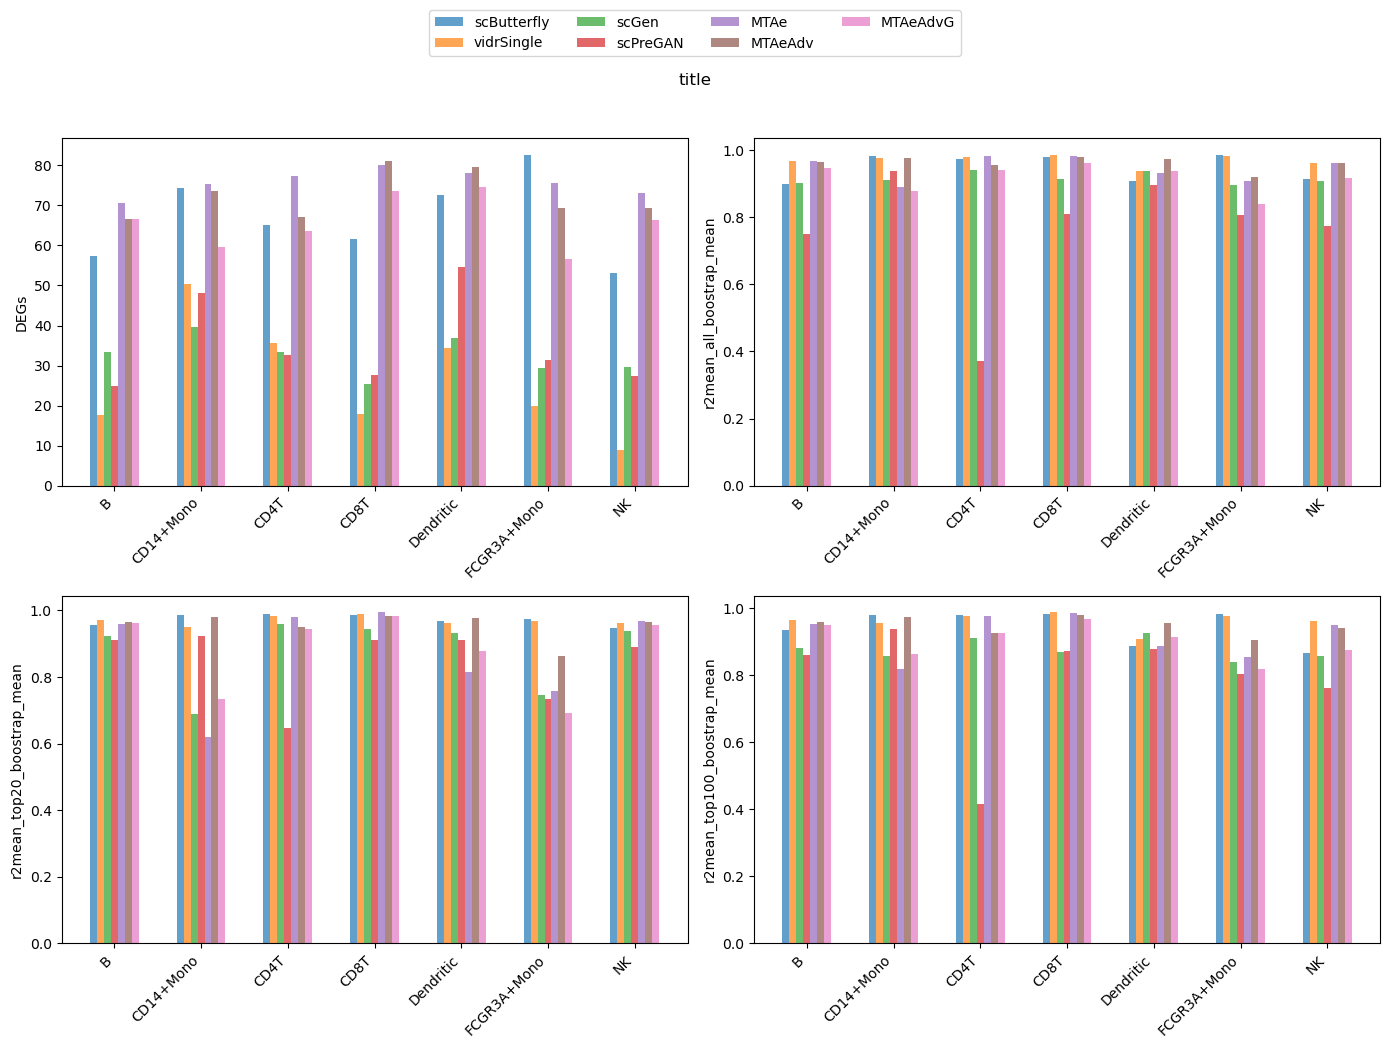
\includegraphics[width=.85\textwidth]{selected_benchmarking_cell_type_baseline_metrics_pbmc.png}
    \caption{Baseline metrics of multi-task and literature models for the Kang et al. \cite{kanaGenerativeModelingSinglecell2023} dataset across cell types}
    \label{fig:selected_pbmc_baseline}
\end{figure}

\begin{figure}[h!]
    \centering
    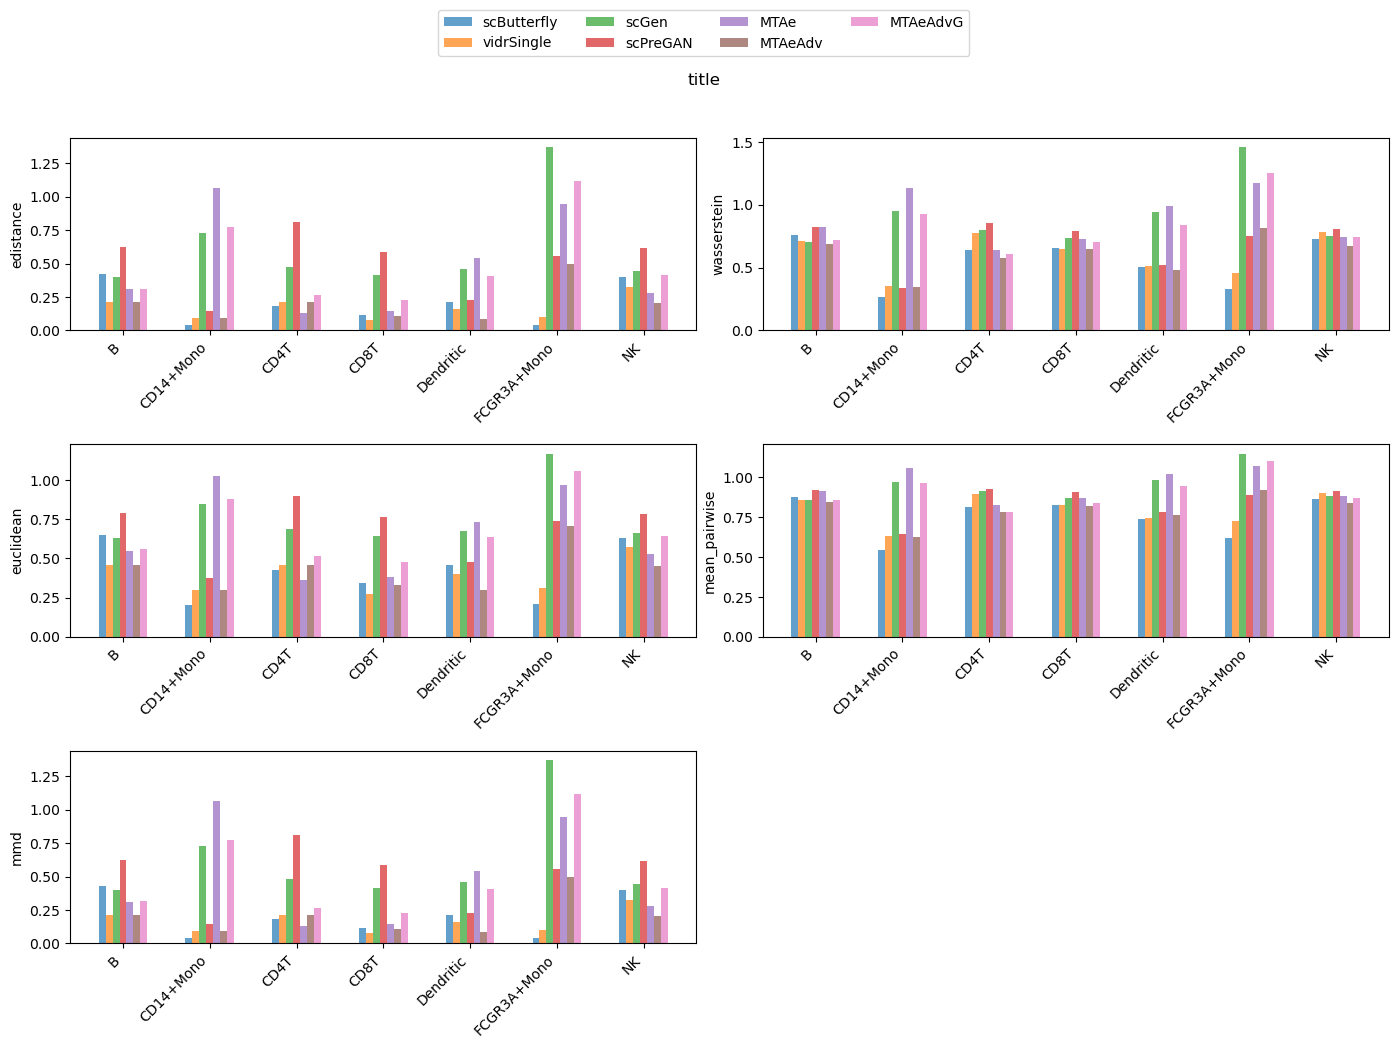
\includegraphics[width=.85\textwidth]{selected_benchmarking_cell_type_distance_metrics_pbmc.png}
    \caption{Distance metrics of multi-task and literature models for the Kang et al. \cite{kanaGenerativeModelingSinglecell2023} dataset across cell types}
    \label{fig:selected_pbmc_distance}
\end{figure}


\begin{figure}[h!]
    \centering
    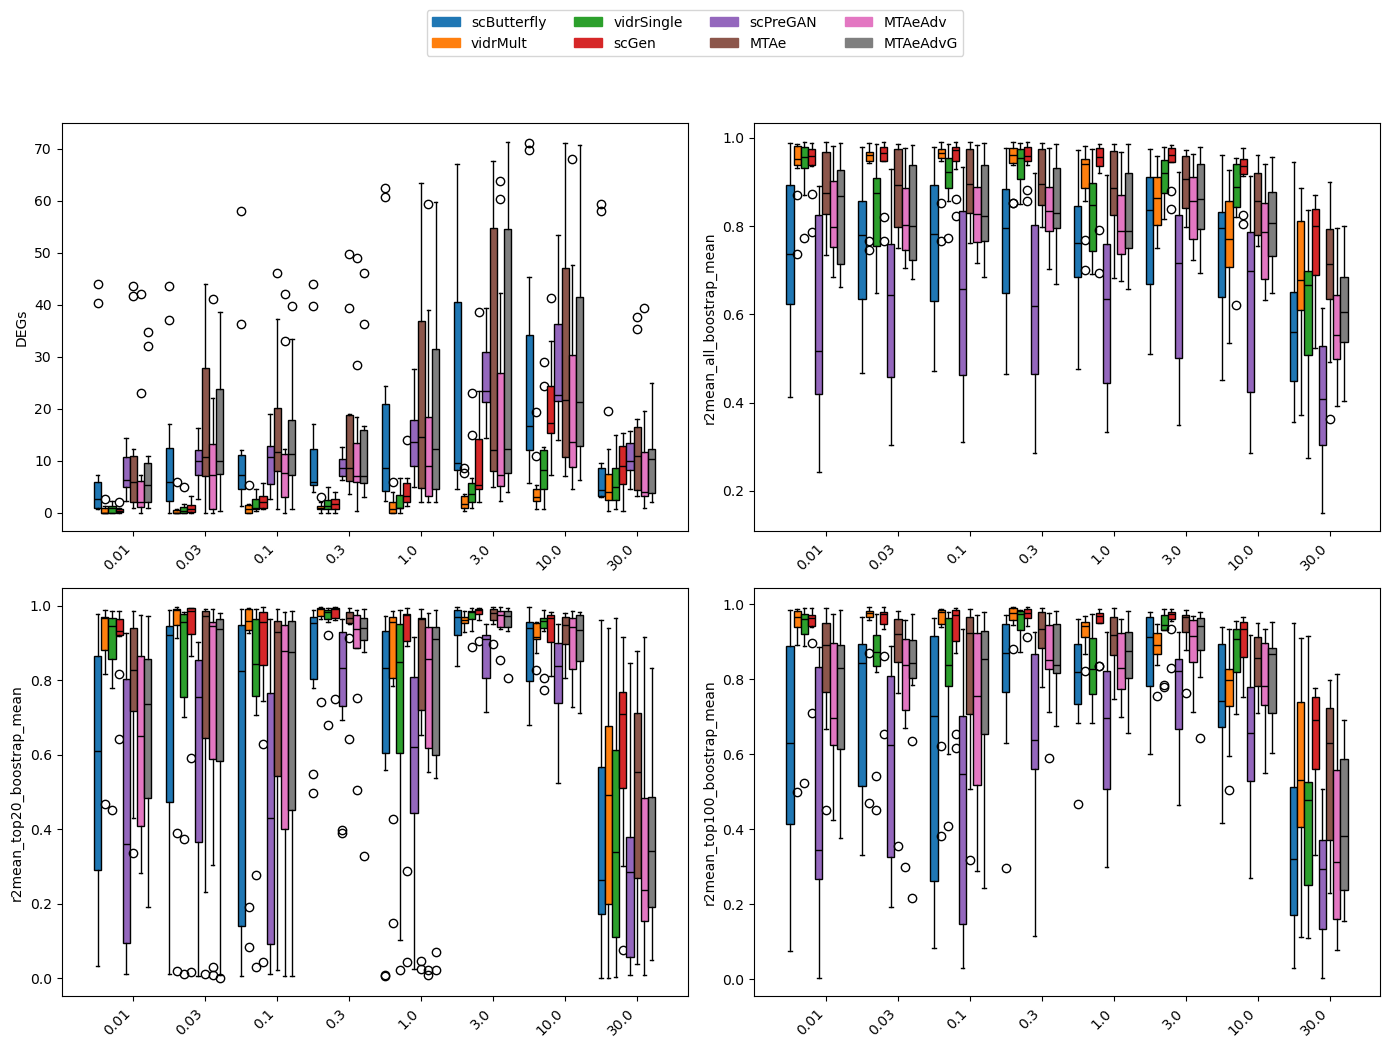
\includegraphics[width=.85\textwidth]{selected_benchmarking_doses_baseline_metrics_nault.png}
    \caption{Baseline metrics of multi-task and literature models for the Nault et al. \cite{nault2021single,nault2022benchmarking} dataset across dosages}
    \label{fig:selected_nault_doses_baseline}
\end{figure}

\begin{figure}[h!]
    \centering
    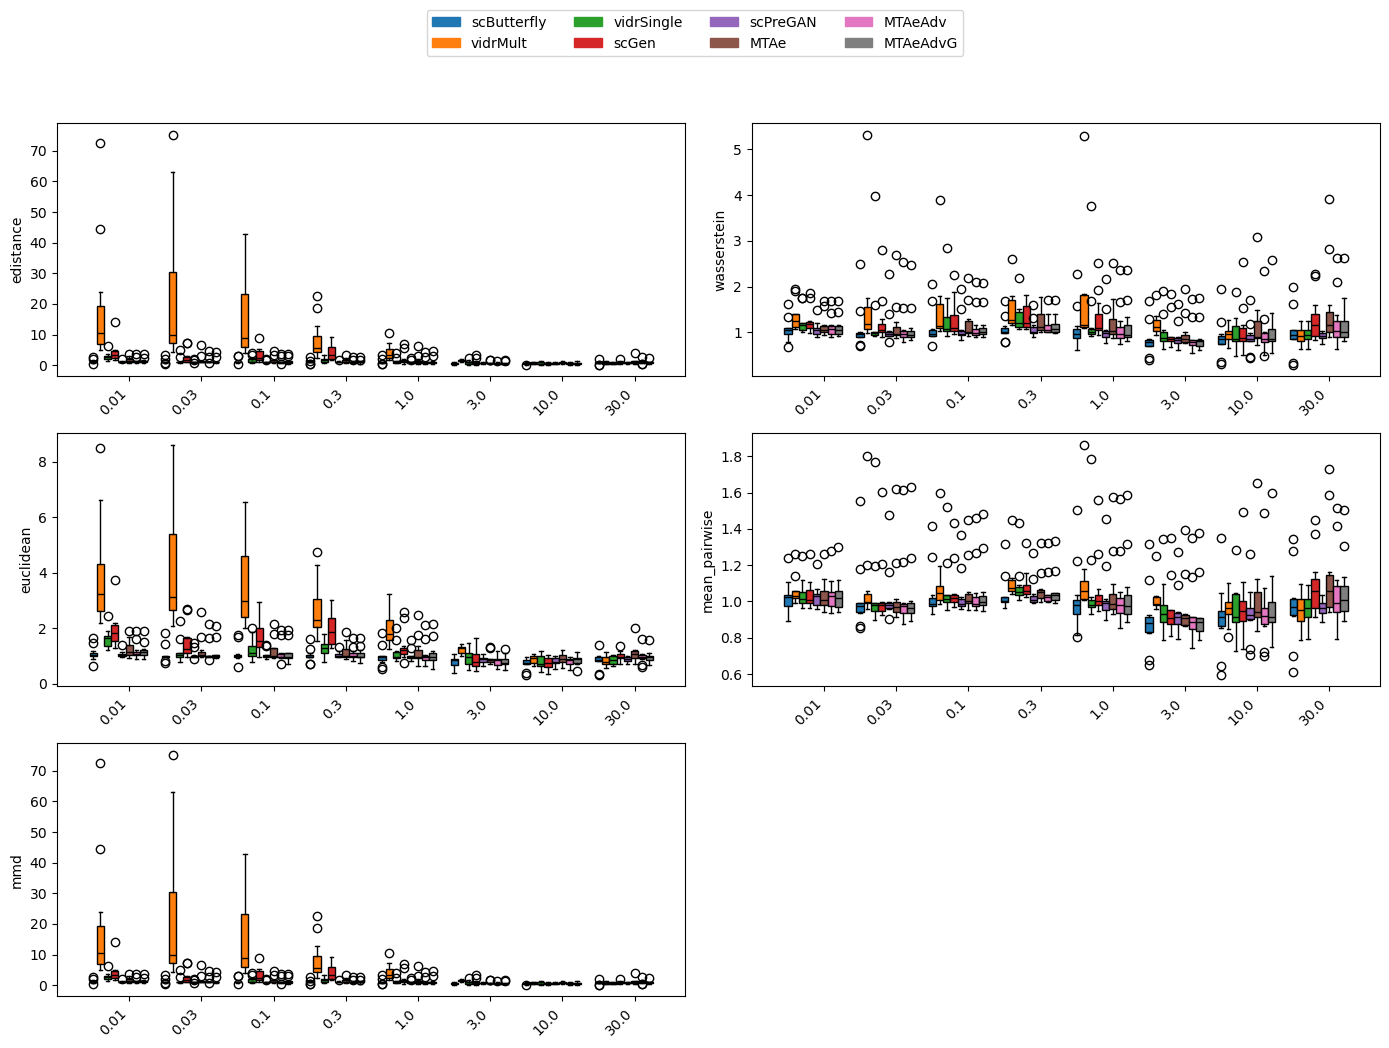
\includegraphics[width=.85\textwidth]{selected_benchmarking_doses_distance_metrics_nault.png}
    \caption{Distance metrics of multi-task and literature models for the Nault et al. \cite{nault2021single,nault2022benchmarking} dataset across dosages}
    \label{fig:selected_nault_doses_distance}
\end{figure}


\begin{figure}[h!]
    \centering
    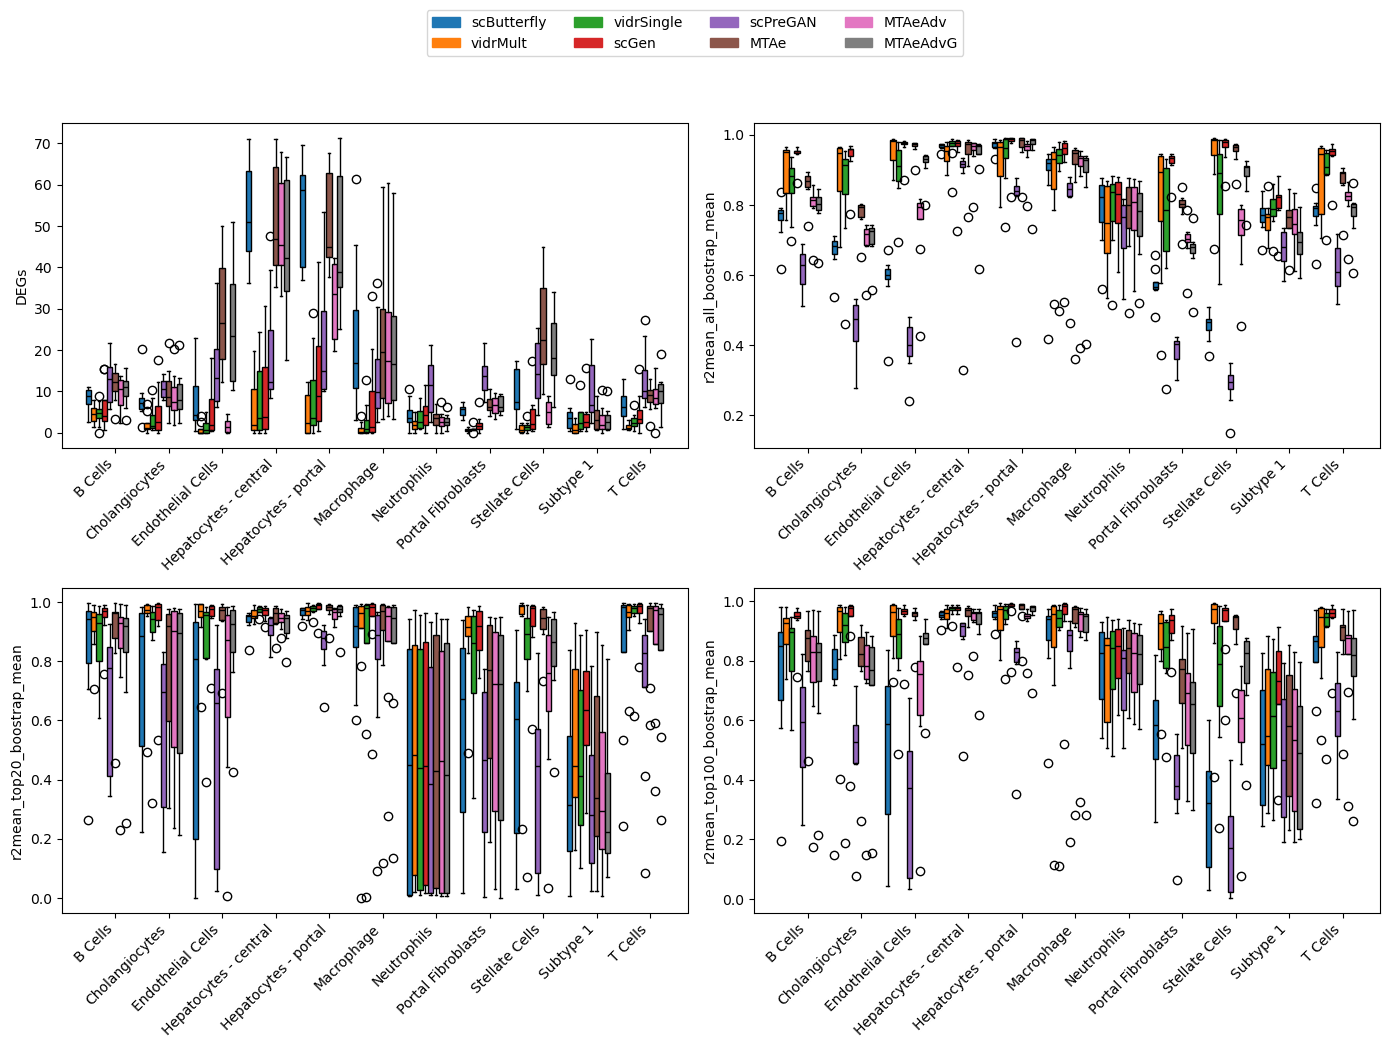
\includegraphics[width=.85\textwidth]{selected_benchmarking_cell_type_baseline_metrics_nault.png}
    \caption{Baseline metrics of multi-task and literature models for the Nault et al. \cite{nault2021single,nault2022benchmarking} dataset across cell types}
    \label{fig:selected_nault_cell_type_baseline}
\end{figure}


\begin{figure}[h!]
    \centering
    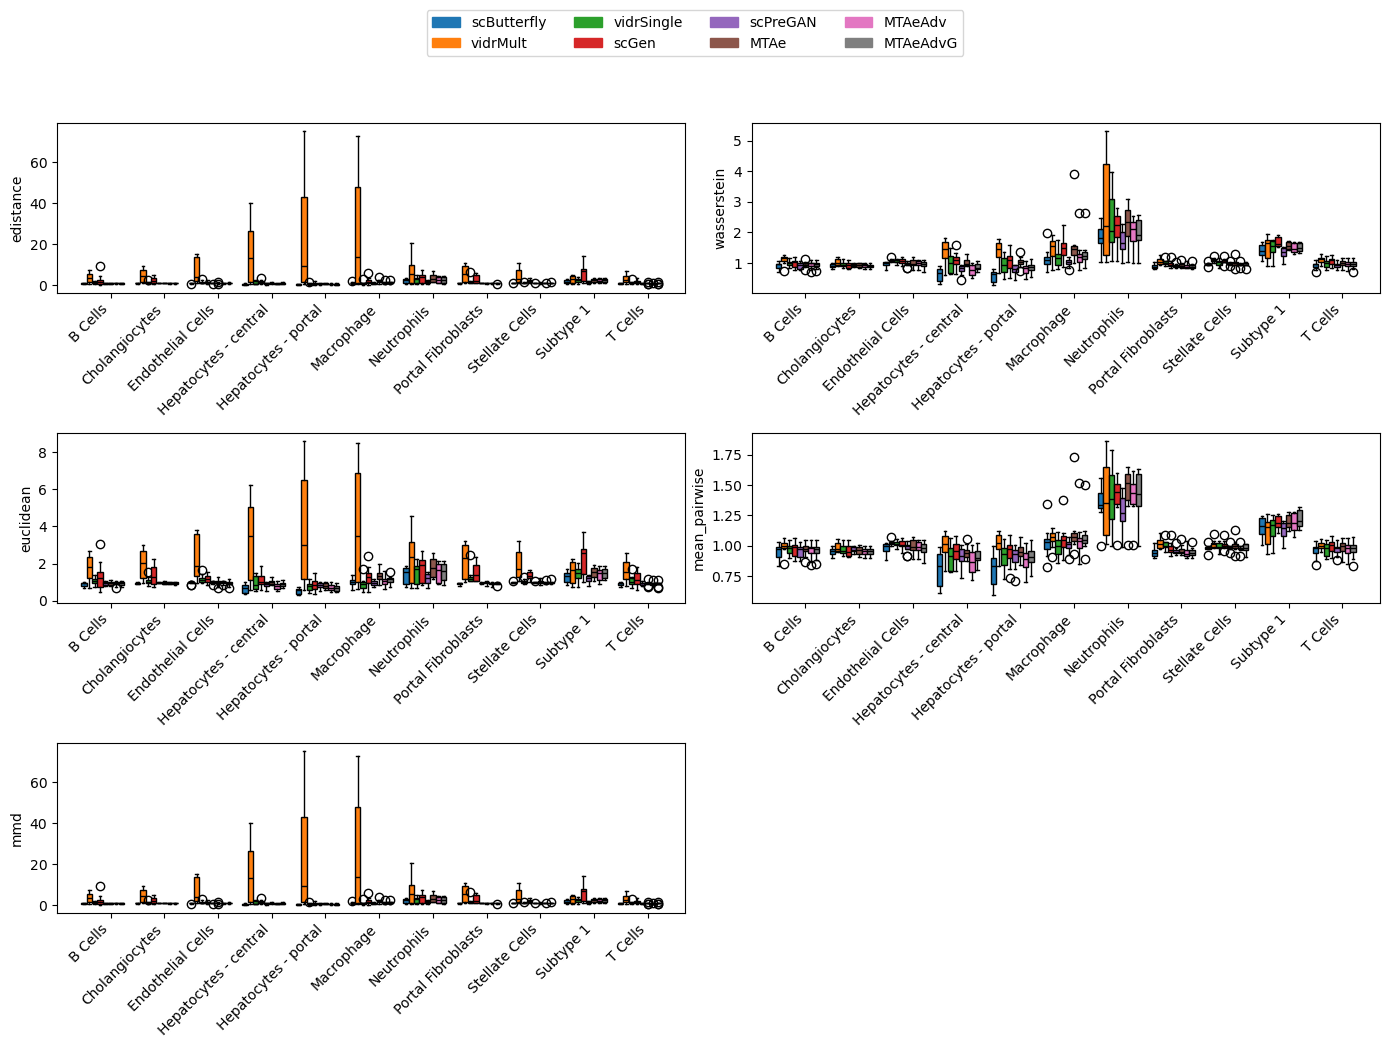
\includegraphics[width=.85\textwidth]{selected_benchmarking_cell_type_distance_metrics_nault.png}
    \caption{Distance metrics of multi-task and literature models for the Nault et al. \cite{nault2021single,nault2022benchmarking} dataset across cell types}
    \label{fig:selected_nault_cell_type_distance}
\end{figure}

% dotplots and latent umaps of the selected models comparison


\clearpage

\subsection{Knowledge transfer}

which tasks and why they are important?

\subsection{TODO}

\begin{itemize}
    \item batch effect
    \item interpretability
    \item explainability
    \item integration with multiple omics
\end{itemize}

\section{Conclusions}

We have validated the potential of scButterfly to perturbation modeling with the multi-dosage dataset of Nault et al. \cite{nault2021single,nault2022benchmarking}, an addition of the author's study that is based only on the dataset of Kang et al. \cite{kanaGenerativeModelingSinglecell2023}. We have proposed multi-task architectures that can be used for perturbation modeling, and we have benchmarked them against the state-of-the-art models in the field. The results show that our models outperform or are comparable to the state-of-the-art models in the field.


\section{Future work}


%\chapter{Benchmarking}
\label{ch:chapter1}

\clearpage


\section{Datasets}

\subsection{Nault et al. 2022}

\begin{figure}[h]
    \centering
    \begin{subfigure}[t]{0.49\textwidth}
        \centering
        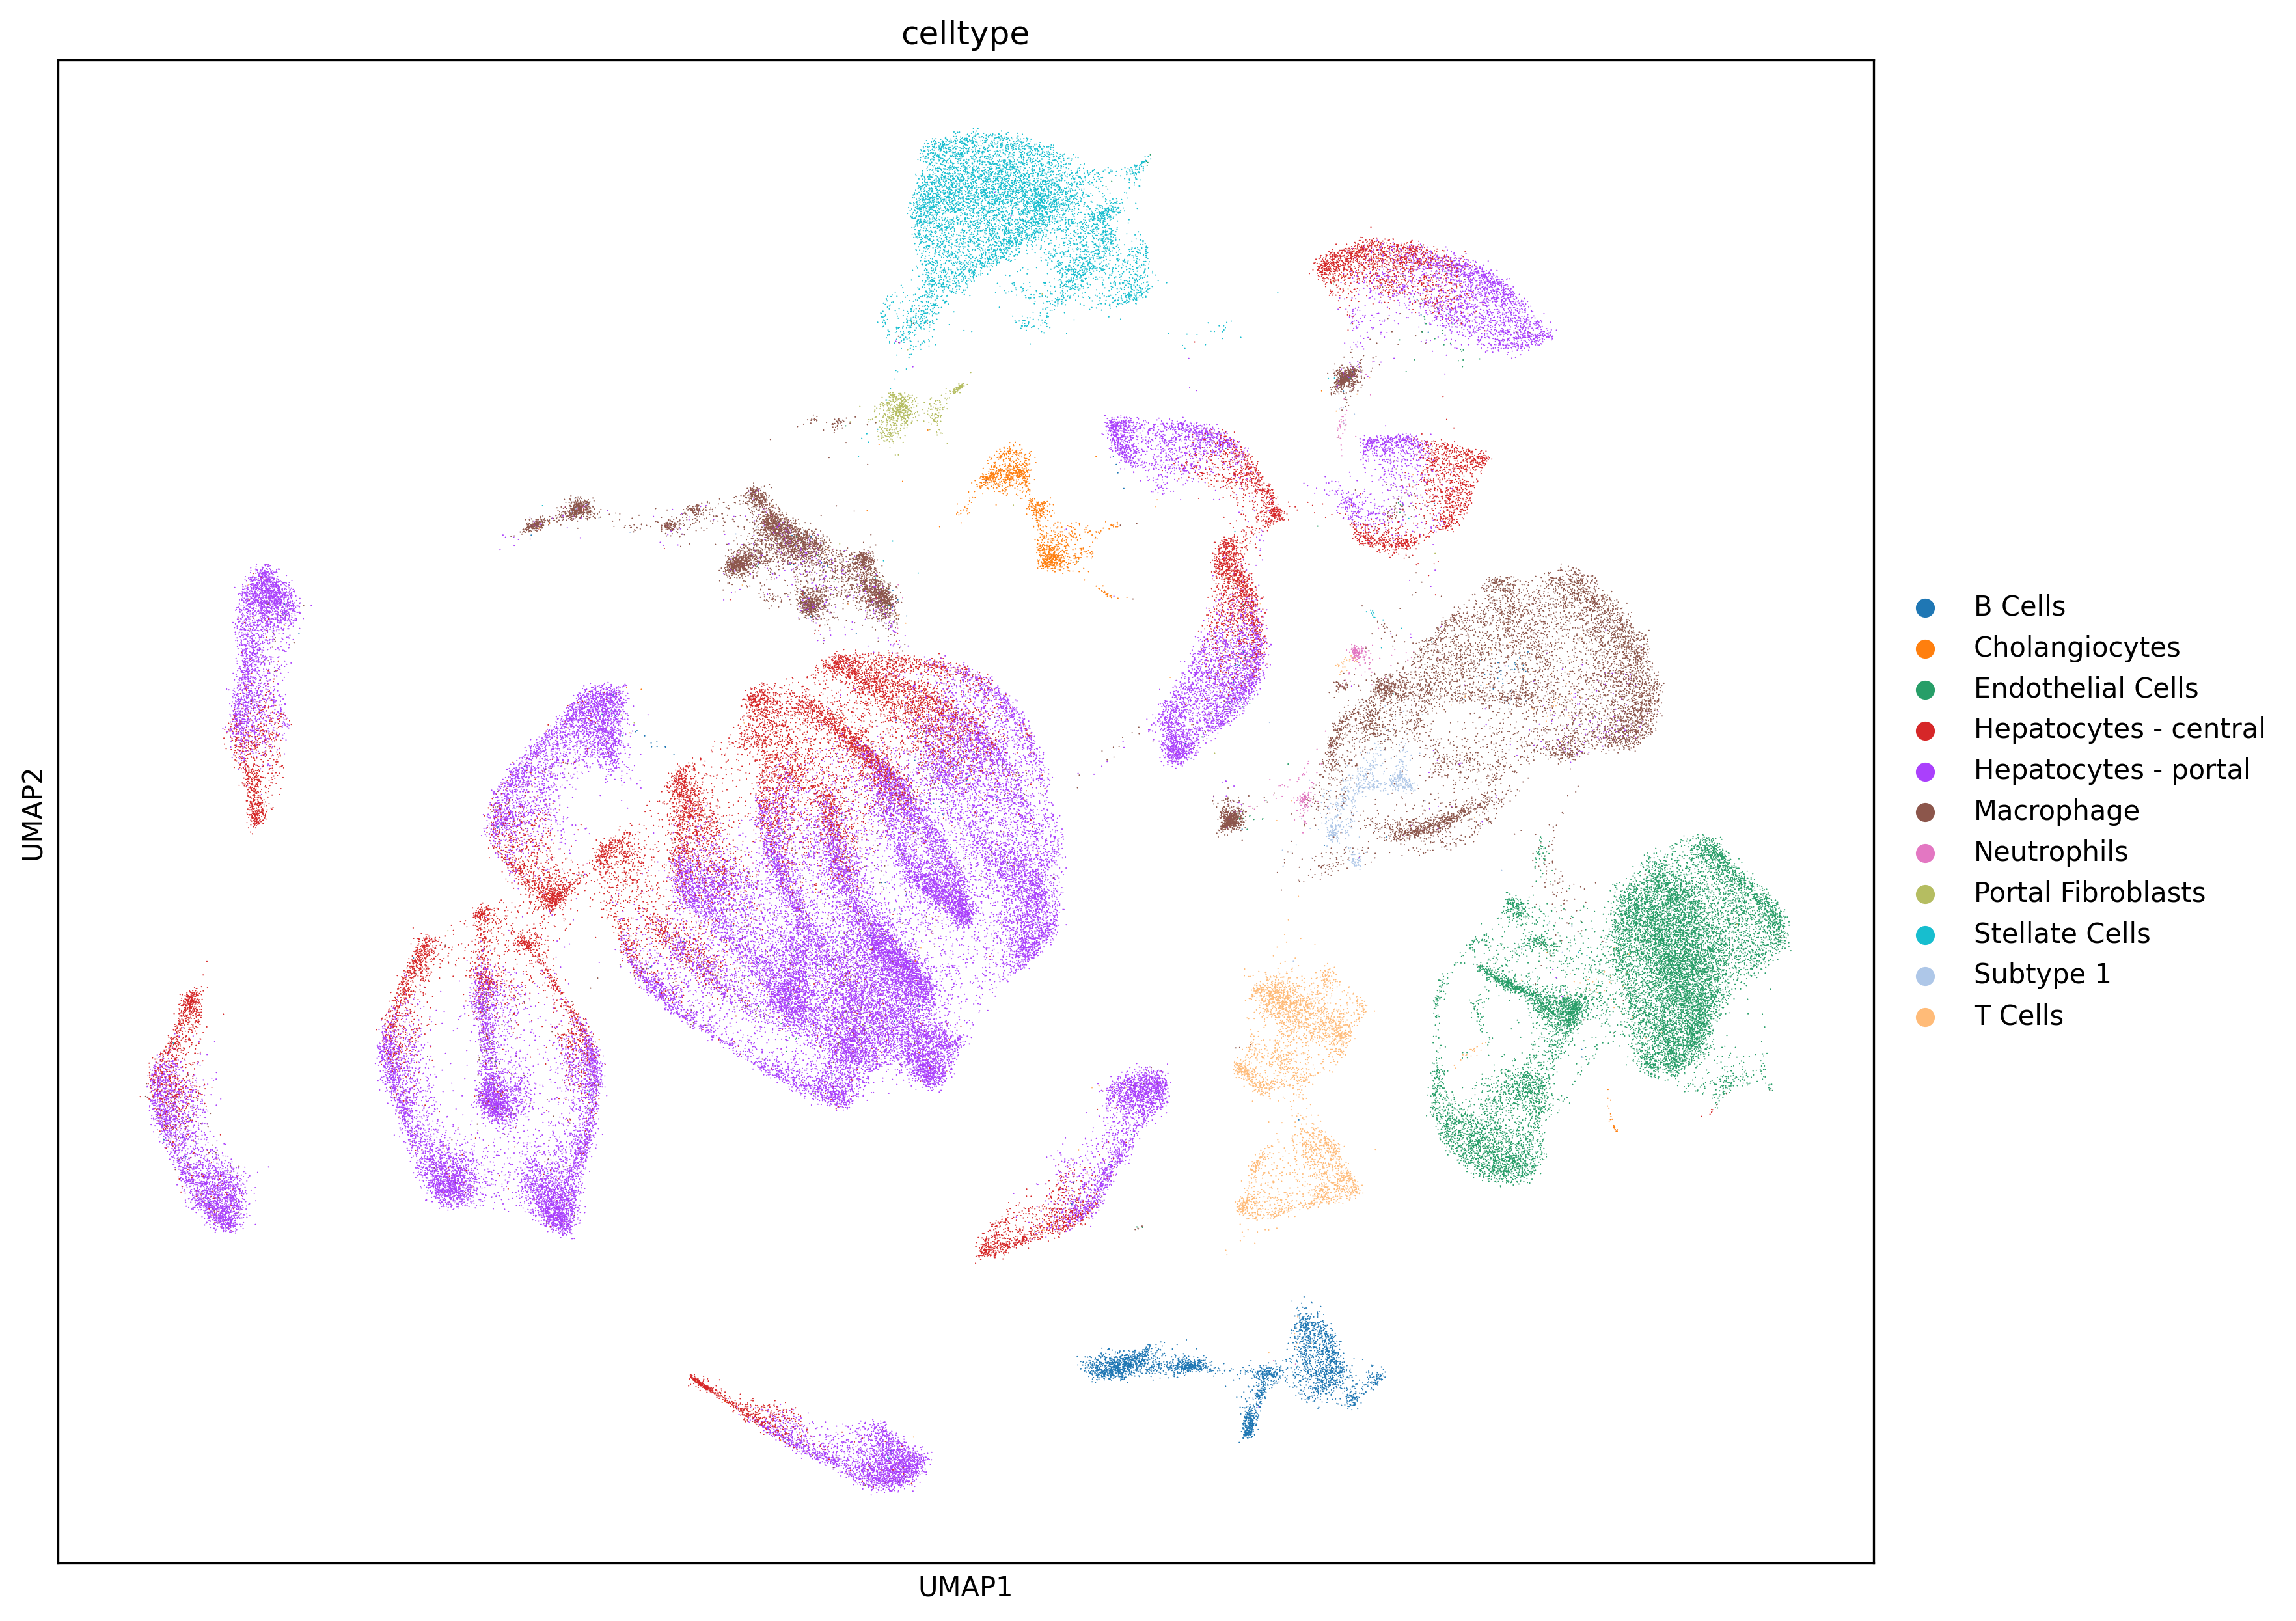
\includegraphics[width=.9\textwidth]{figures/nault_cell_umap.png}
        \caption{}
        \label{fig:figure1}.
    \end{subfigure}%
    \hfill
    \begin{subfigure}[t]{0.49\textwidth}
        \centering
        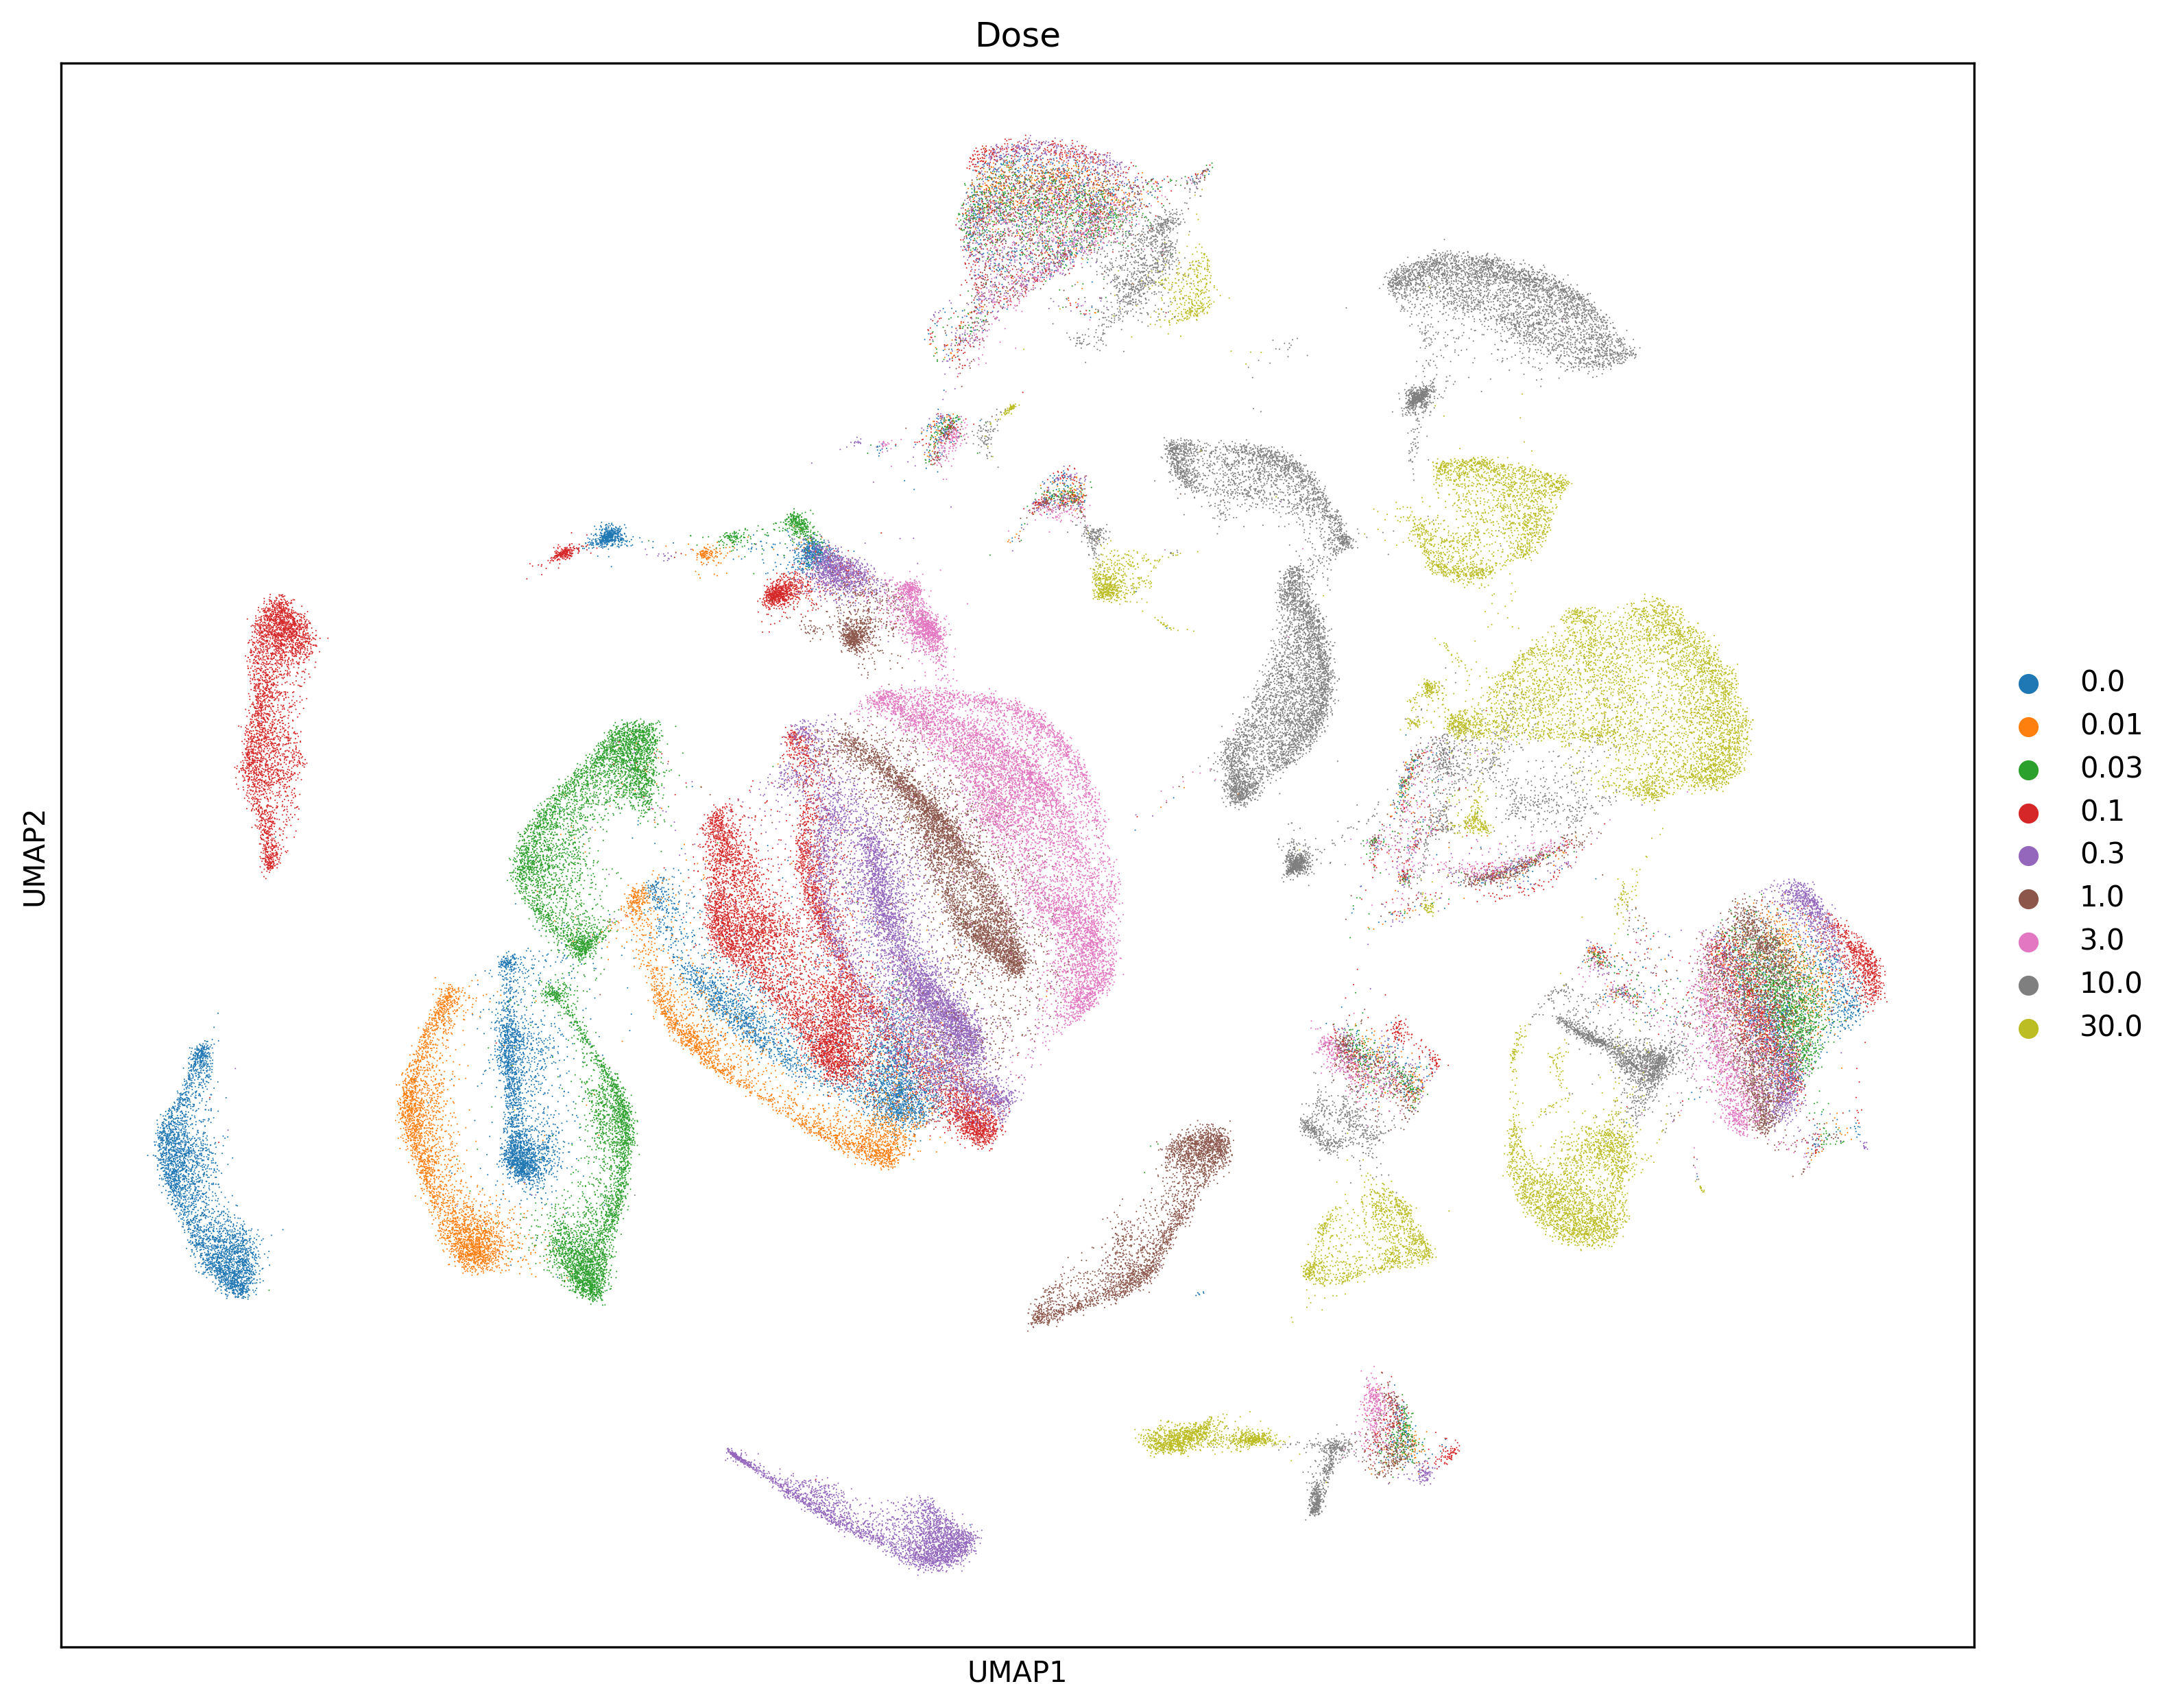
\includegraphics[width=.8\textwidth]{figures/nault_dose_umap.png}
        \caption{}
        \label{fig:figure2}
    \end{subfigure}%
    \hfill
    \begin{subfigure}[b]{\textwidth}
        \centering
        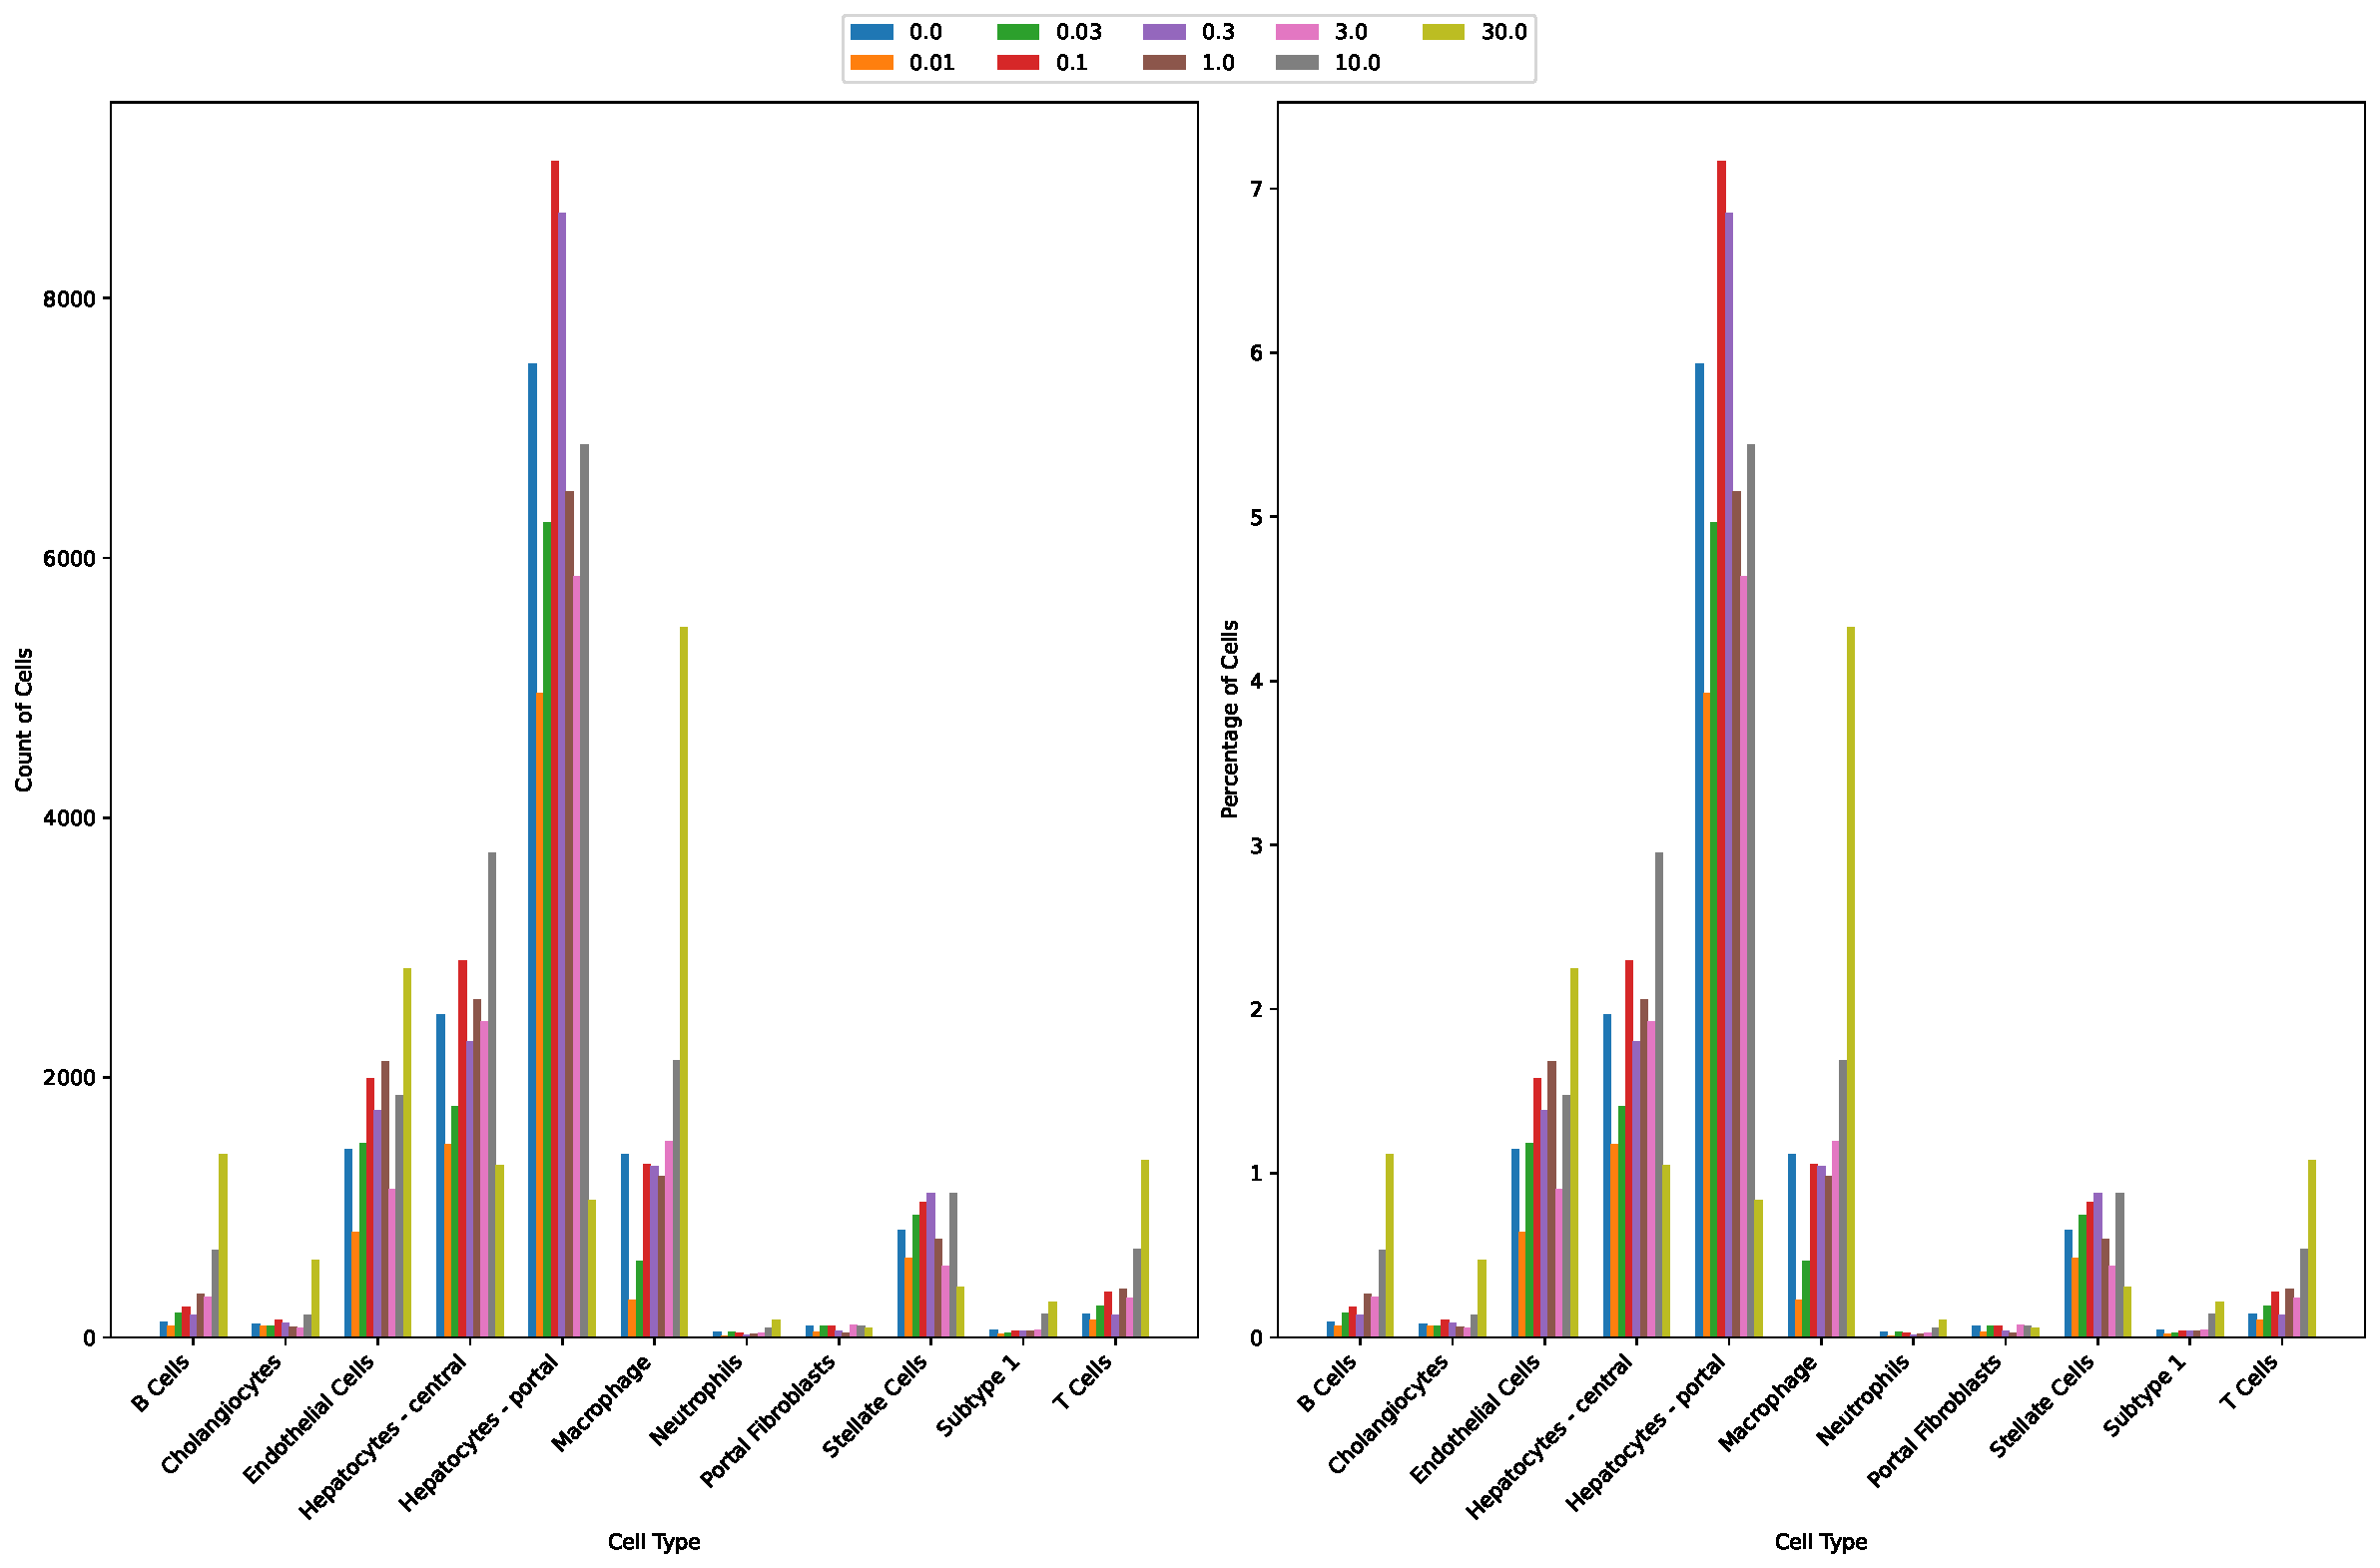
\includegraphics[width=.7\textwidth]{figures/nault_dosages_counts.pdf}
        \caption{}
        \label{fig:figure3}
    \end{subfigure}
    \hfill
    \begin{subfigure}[b]{\textwidth}
        \centering
        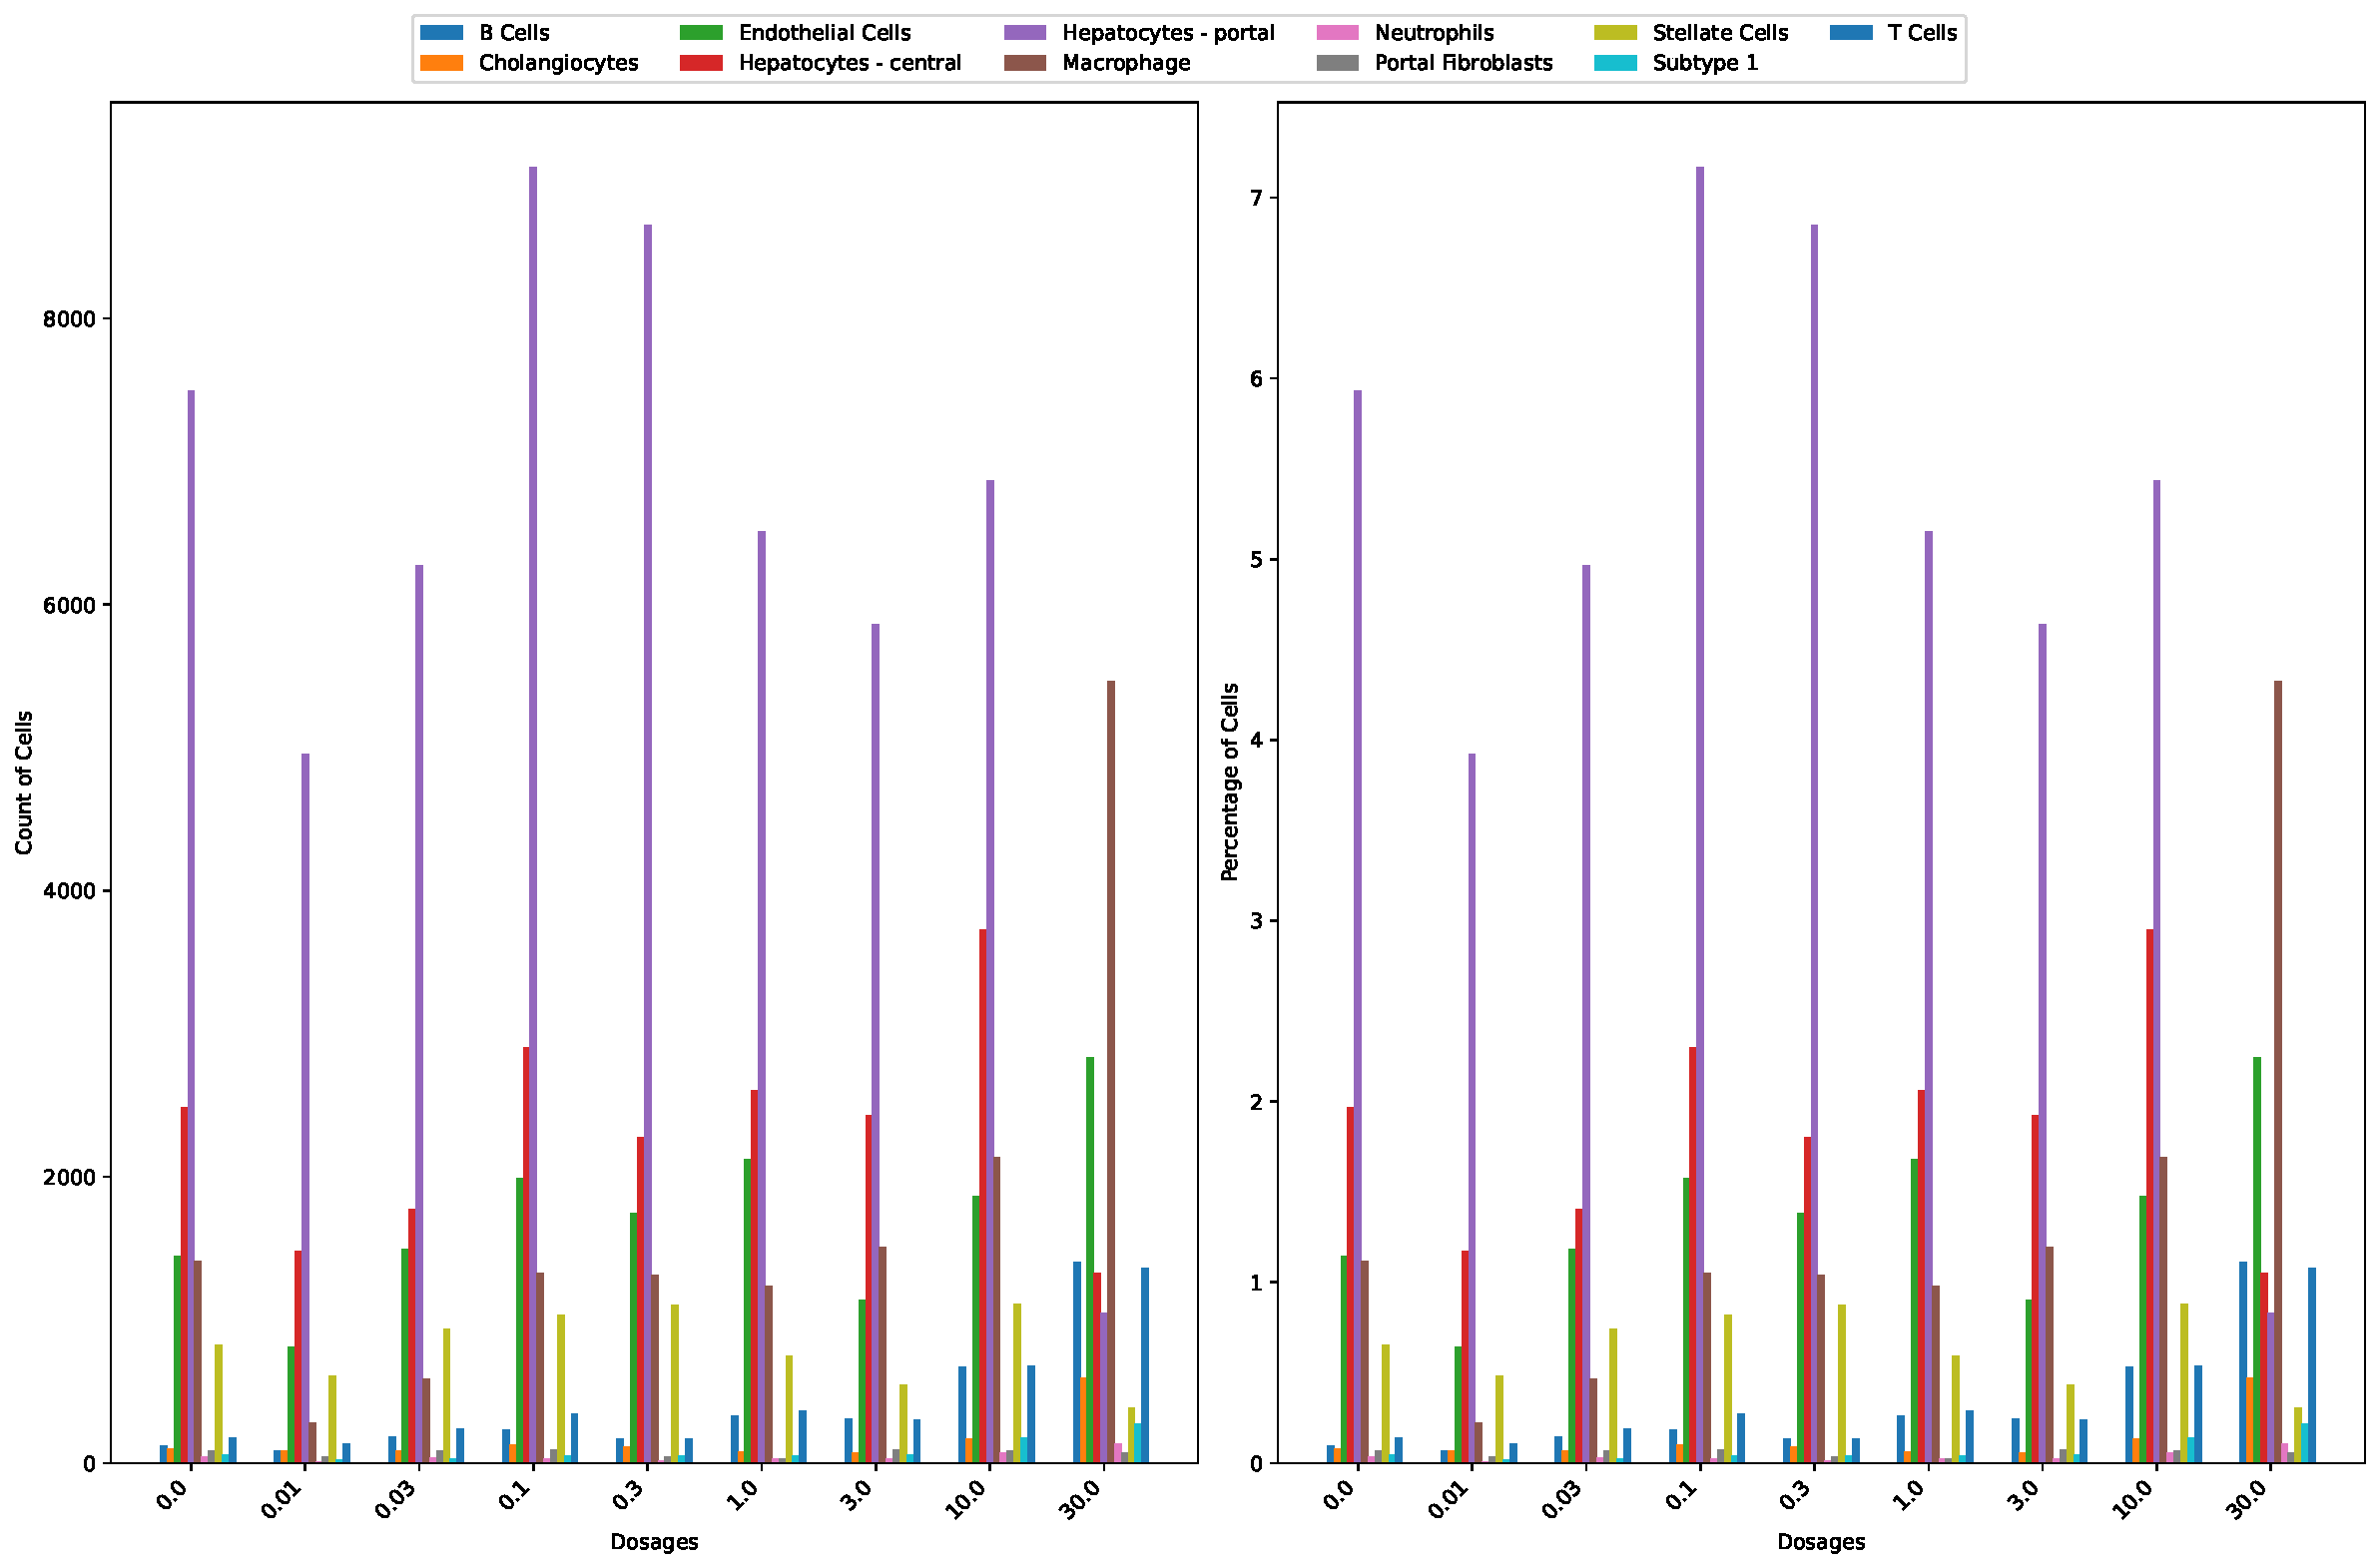
\includegraphics[width=.7\textwidth]{figures/nault_cell_types_counts.pdf}
        \caption{}
        \label{fig:figure4}
    \end{subfigure}    
    \caption{Nault overview}
    \label{fig:combined}
\end{figure}



\begin{figure}
    \centering
    \begin{minipage}{0.4\textwidth}
        \centering
        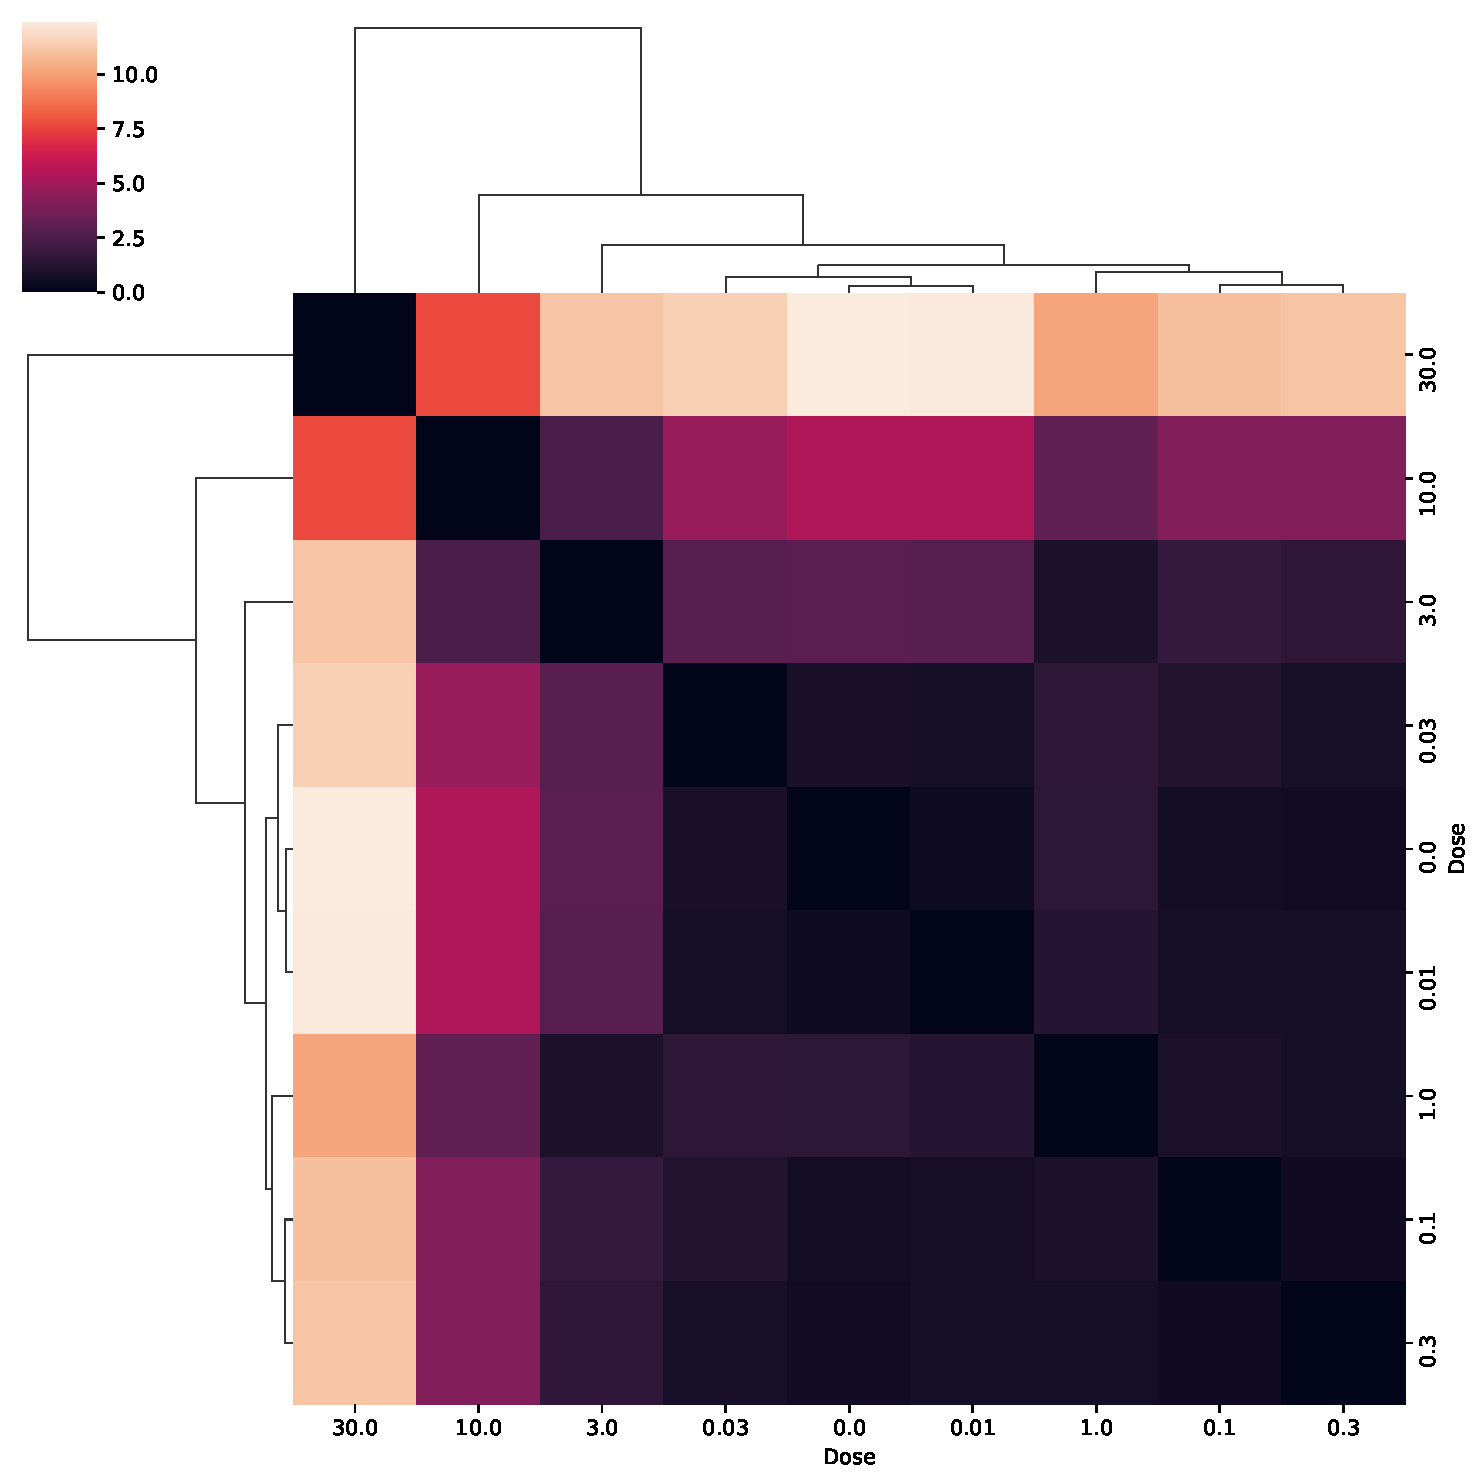
\includegraphics[width=\textwidth]{figures/nault_edistance_clustermap.pdf}
        \caption{E-distance}
    \end{minipage} \hfill
    \begin{minipage}{0.4\textwidth}
        \centering
        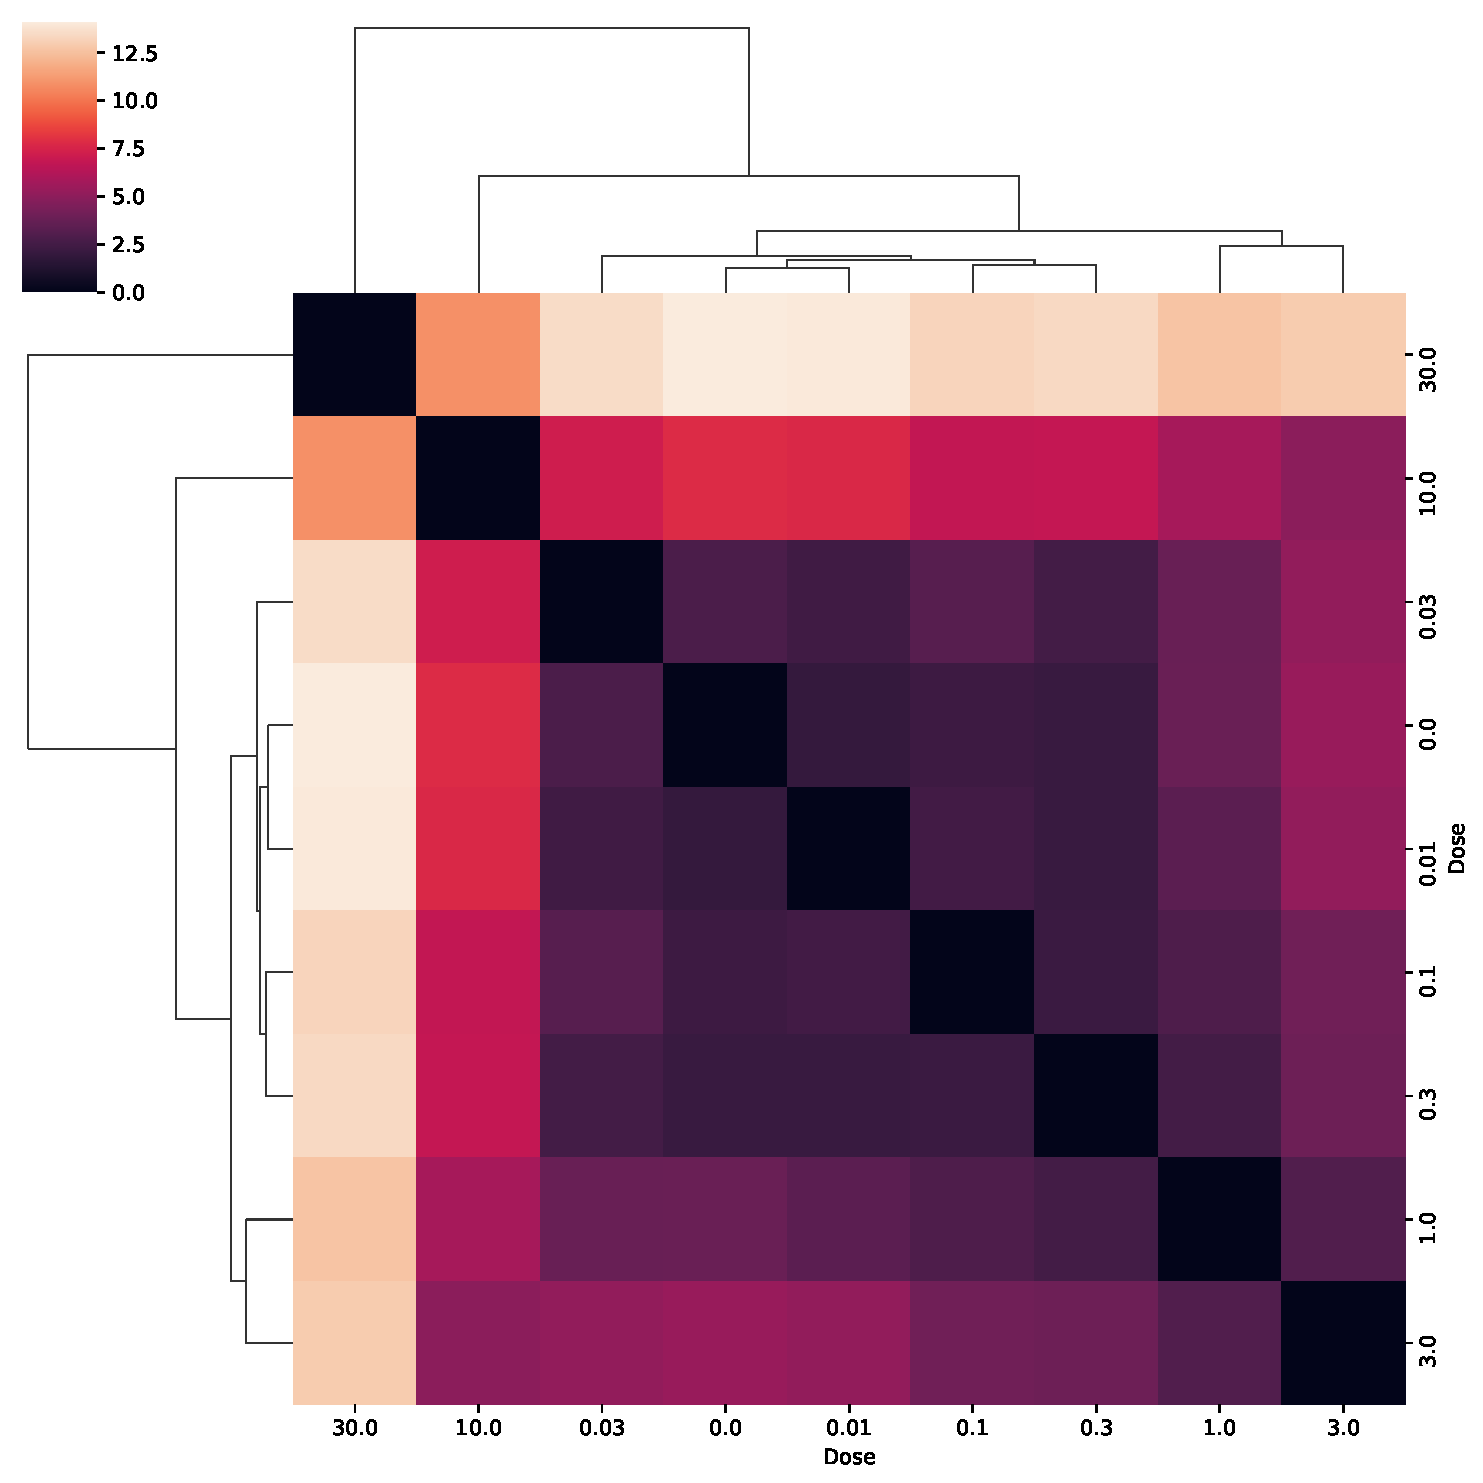
\includegraphics[width=\textwidth]{figures/nault_euclidean_clustermap.pdf}
        \caption{Euclidean}
    \end{minipage}
    \vskip\baselineskip

    \begin{minipage}{0.4\textwidth}
        \centering
        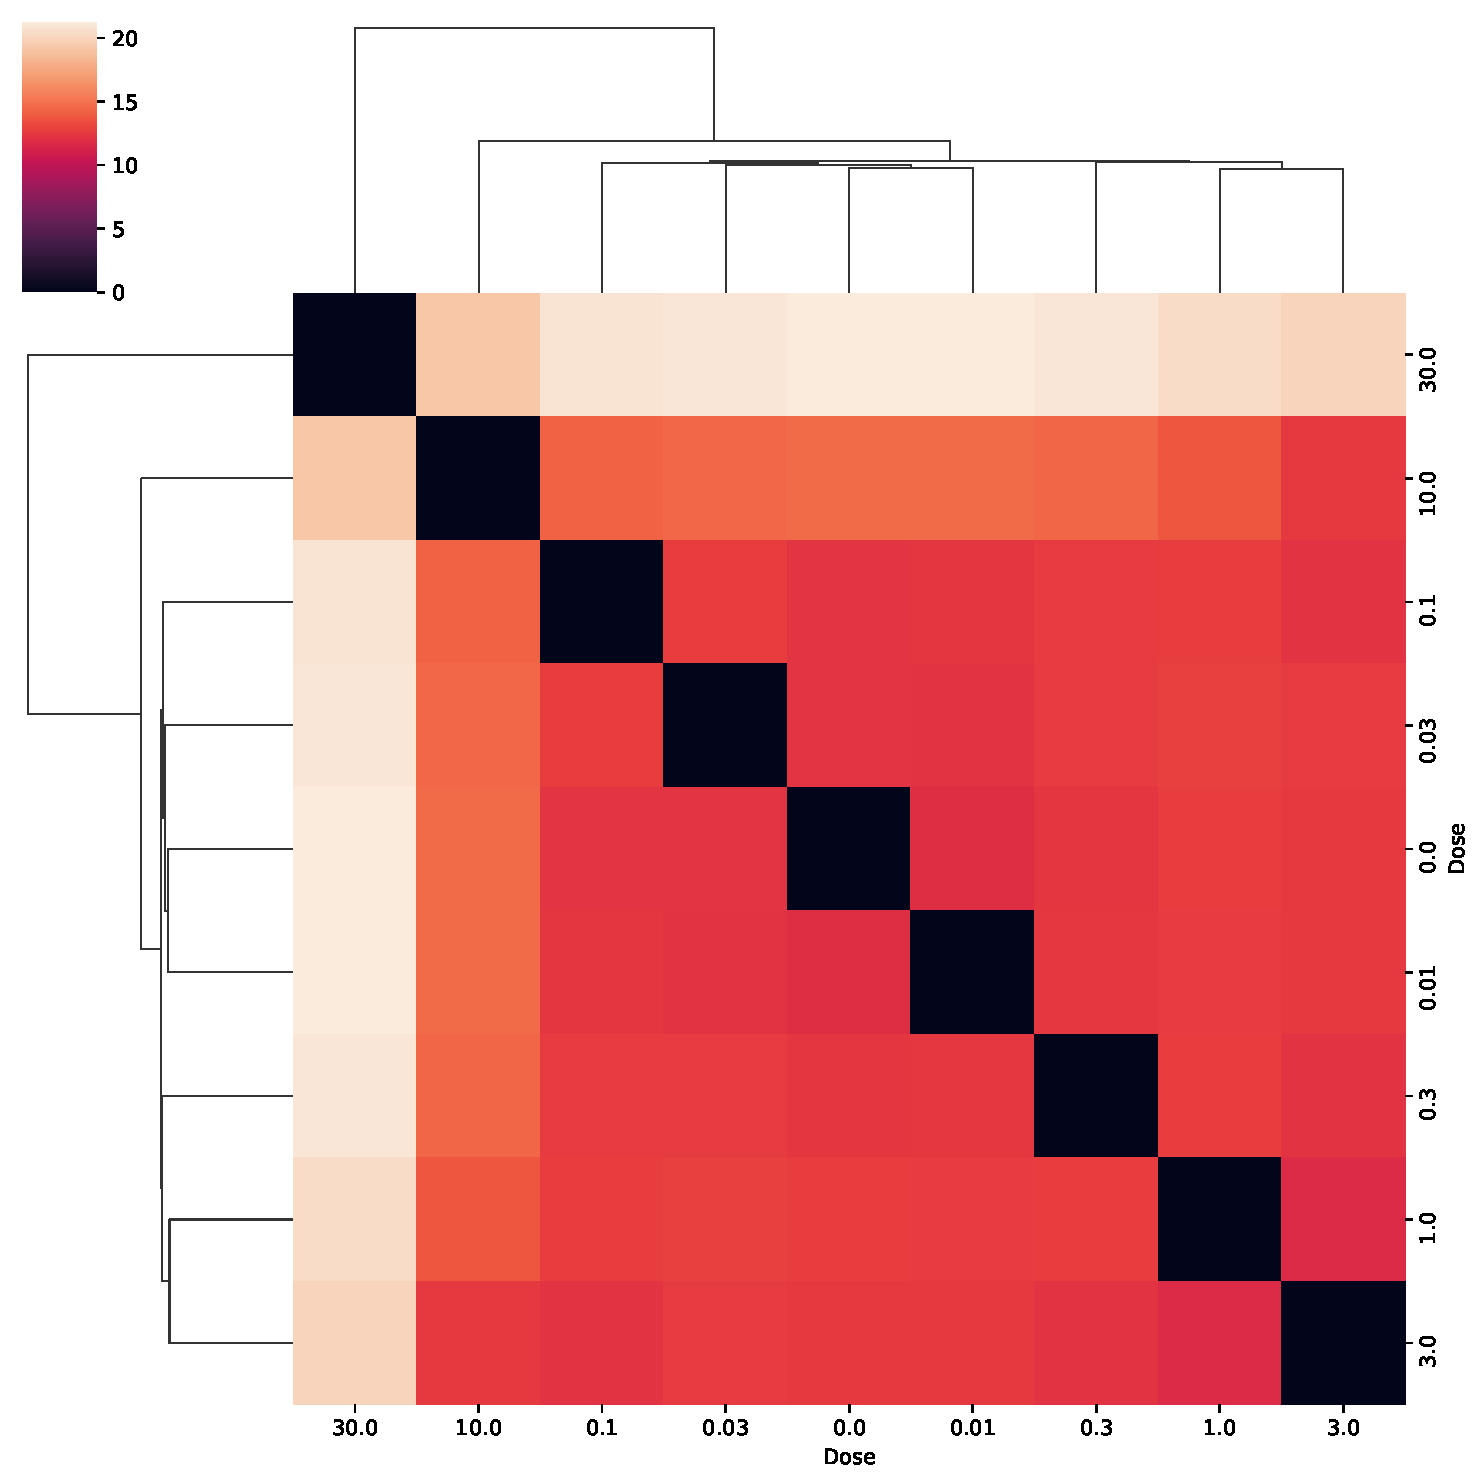
\includegraphics[width=\textwidth]{figures/nault_mean_pairwise_clustermap.pdf}
        \caption{Mean pairwise}
    \end{minipage} \hfill
    \begin{minipage}{0.4\textwidth}
        \centering
        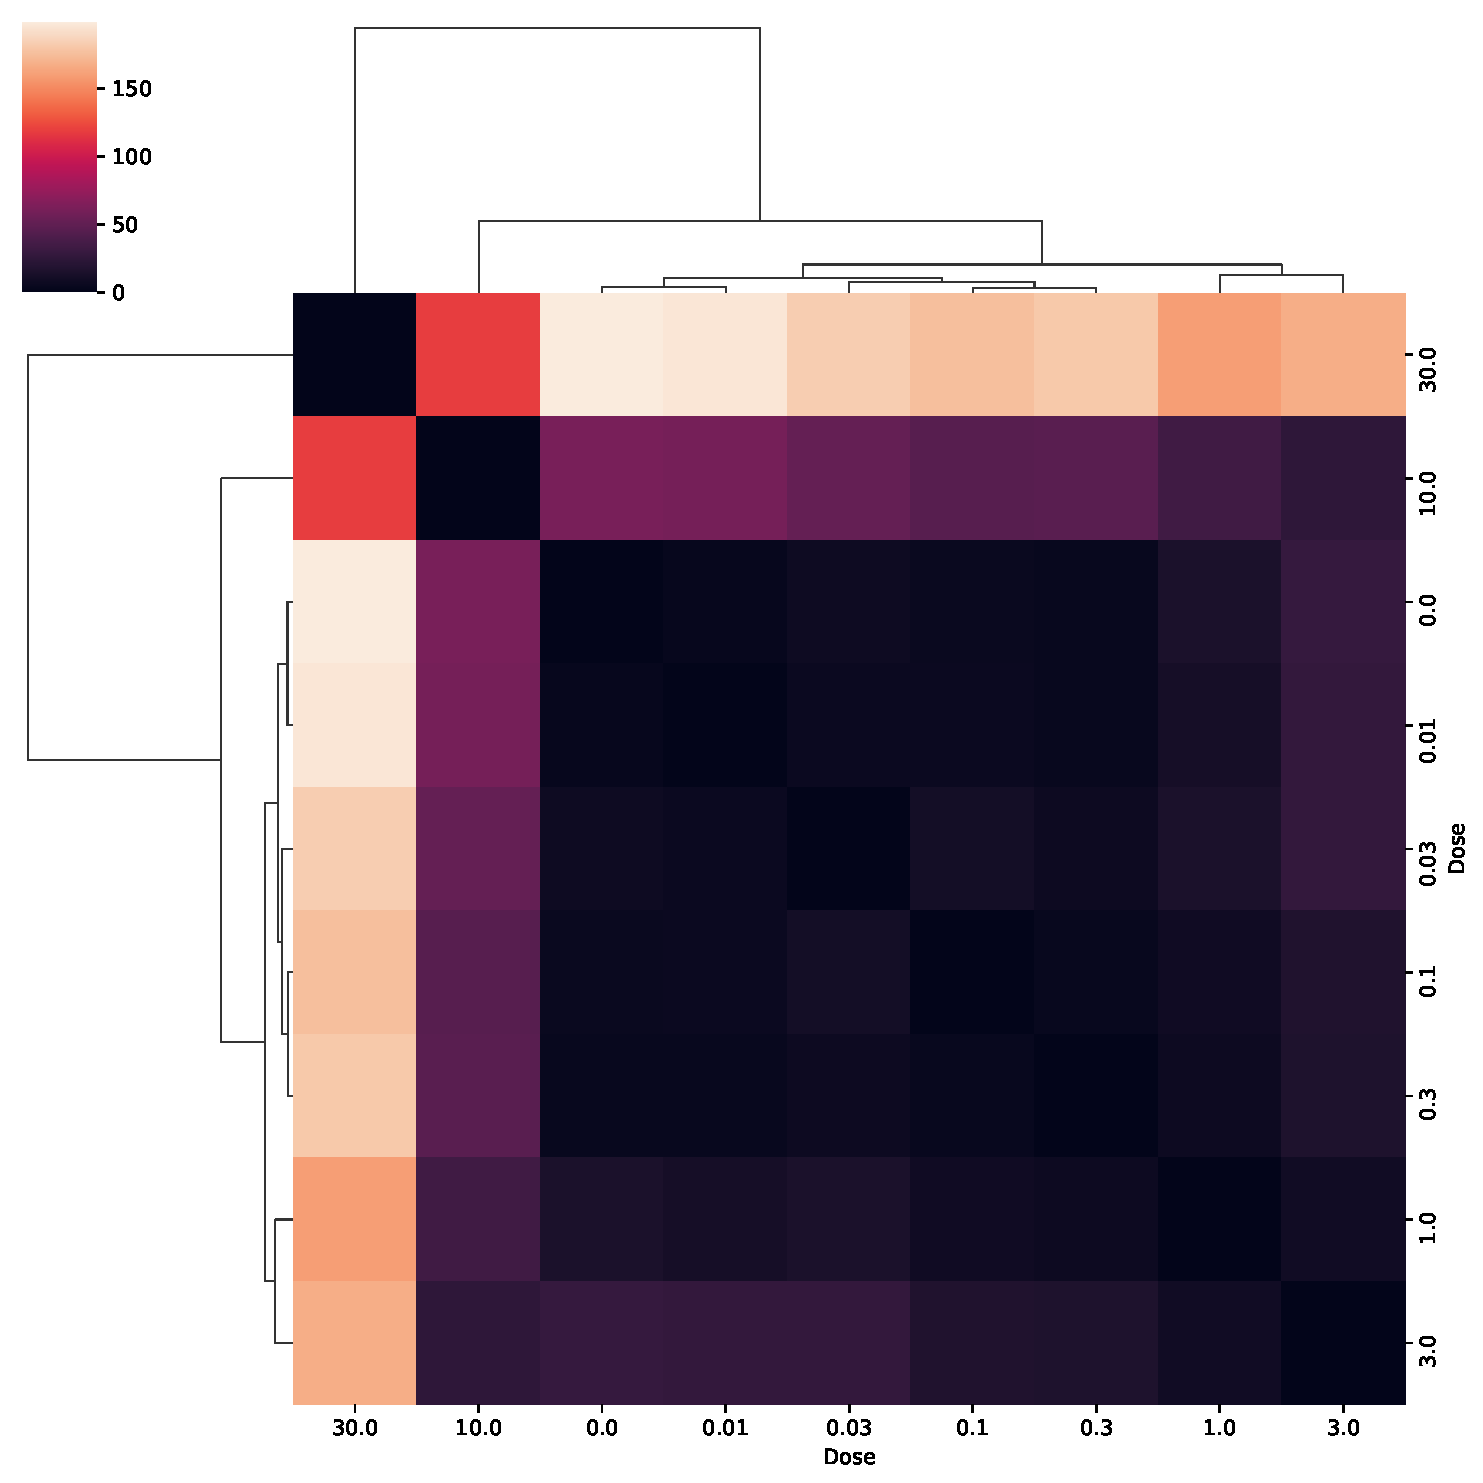
\includegraphics[width=\textwidth]{figures/nault_mmd_clustermap.pdf}
        \caption{MMD}
    \end{minipage}
    \vskip\baselineskip

    \begin{minipage}{0.4\textwidth}
        \centering
        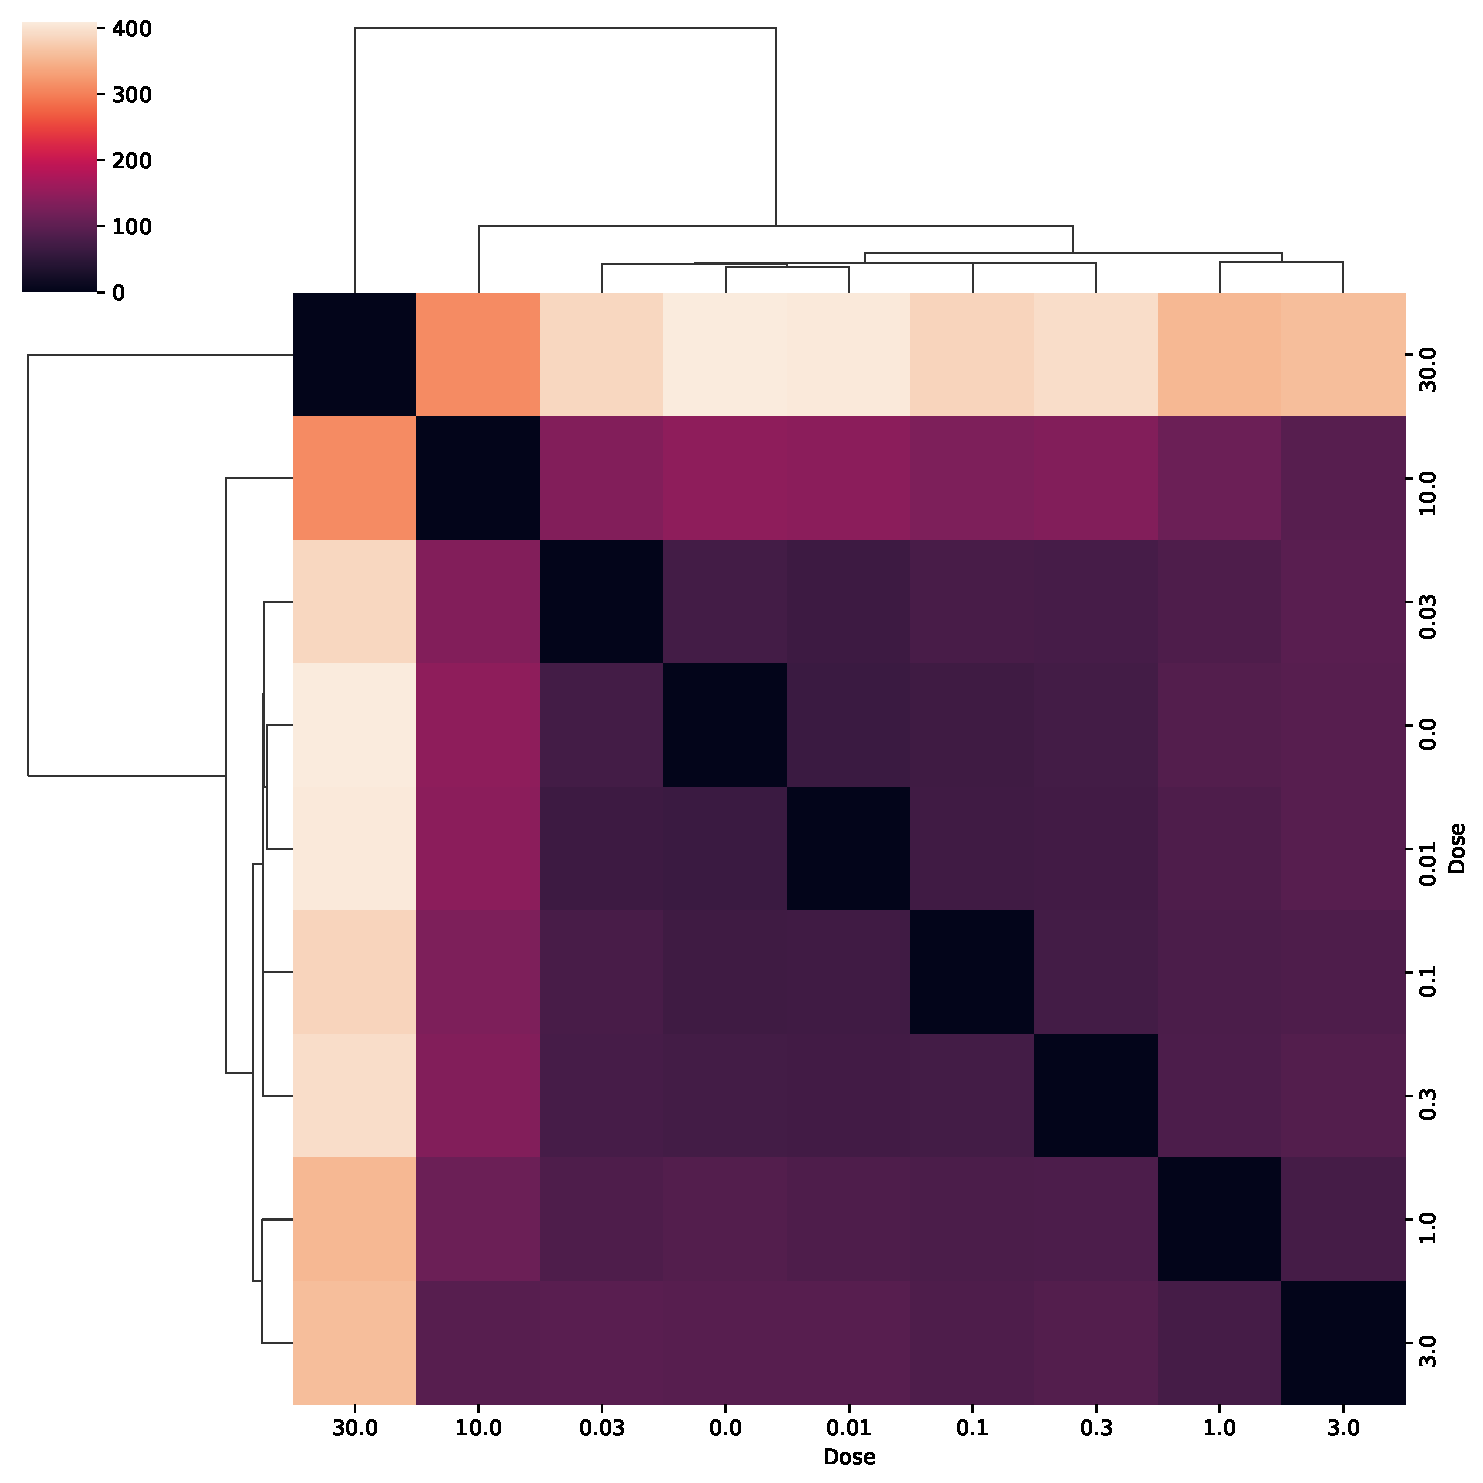
\includegraphics[width=\textwidth]{figures/nault_wasserstein_clustermap.pdf}
        \caption{Wasserstein}
    \end{minipage}
    \caption{Distance metrics across all cell types per dosage}
\end{figure}

\begin{figure}
    \centering
    \begin{minipage}{0.4\textwidth}
        \centering
        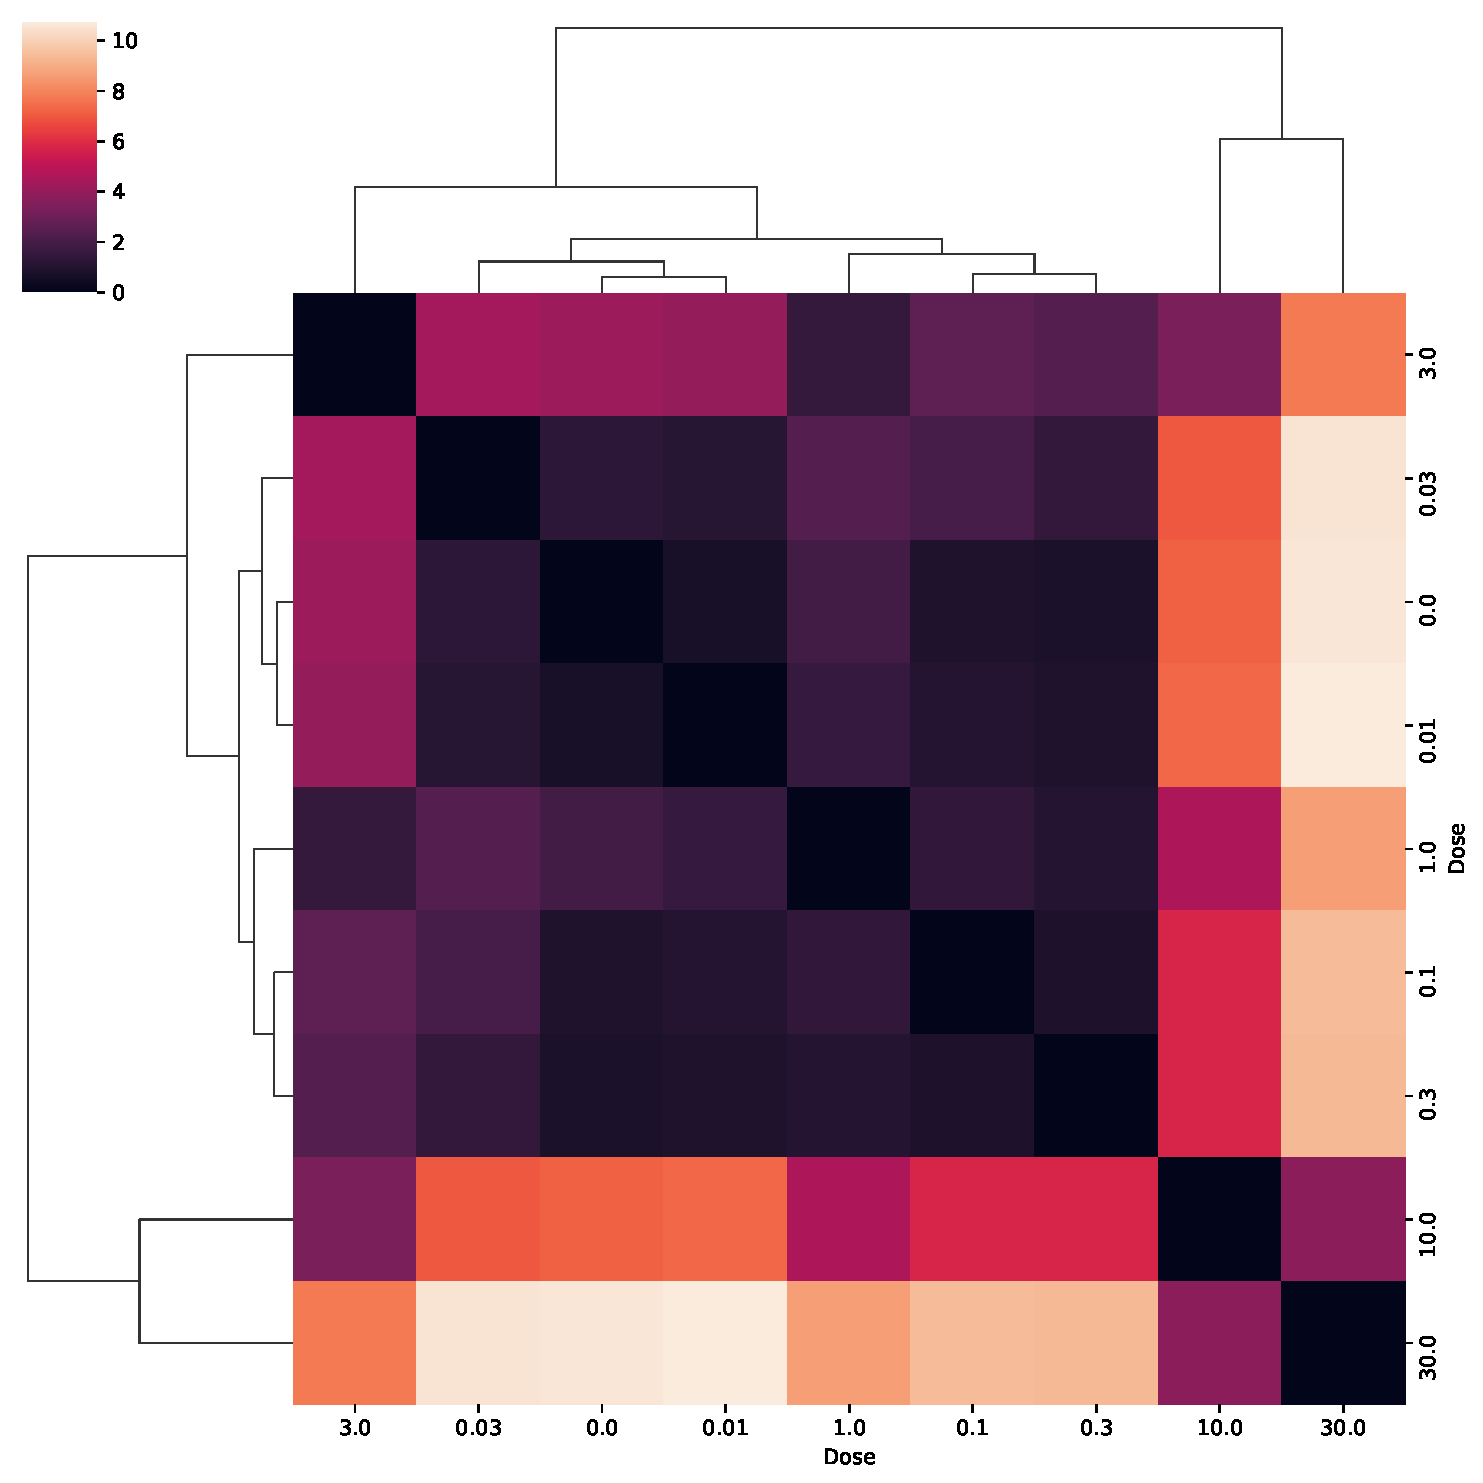
\includegraphics[width=\textwidth]{figures/hepatocytes_edistance_clustermap.pdf}
        \caption{E-distance}
    \end{minipage} \hfill
    \begin{minipage}{0.4\textwidth}
        \centering
        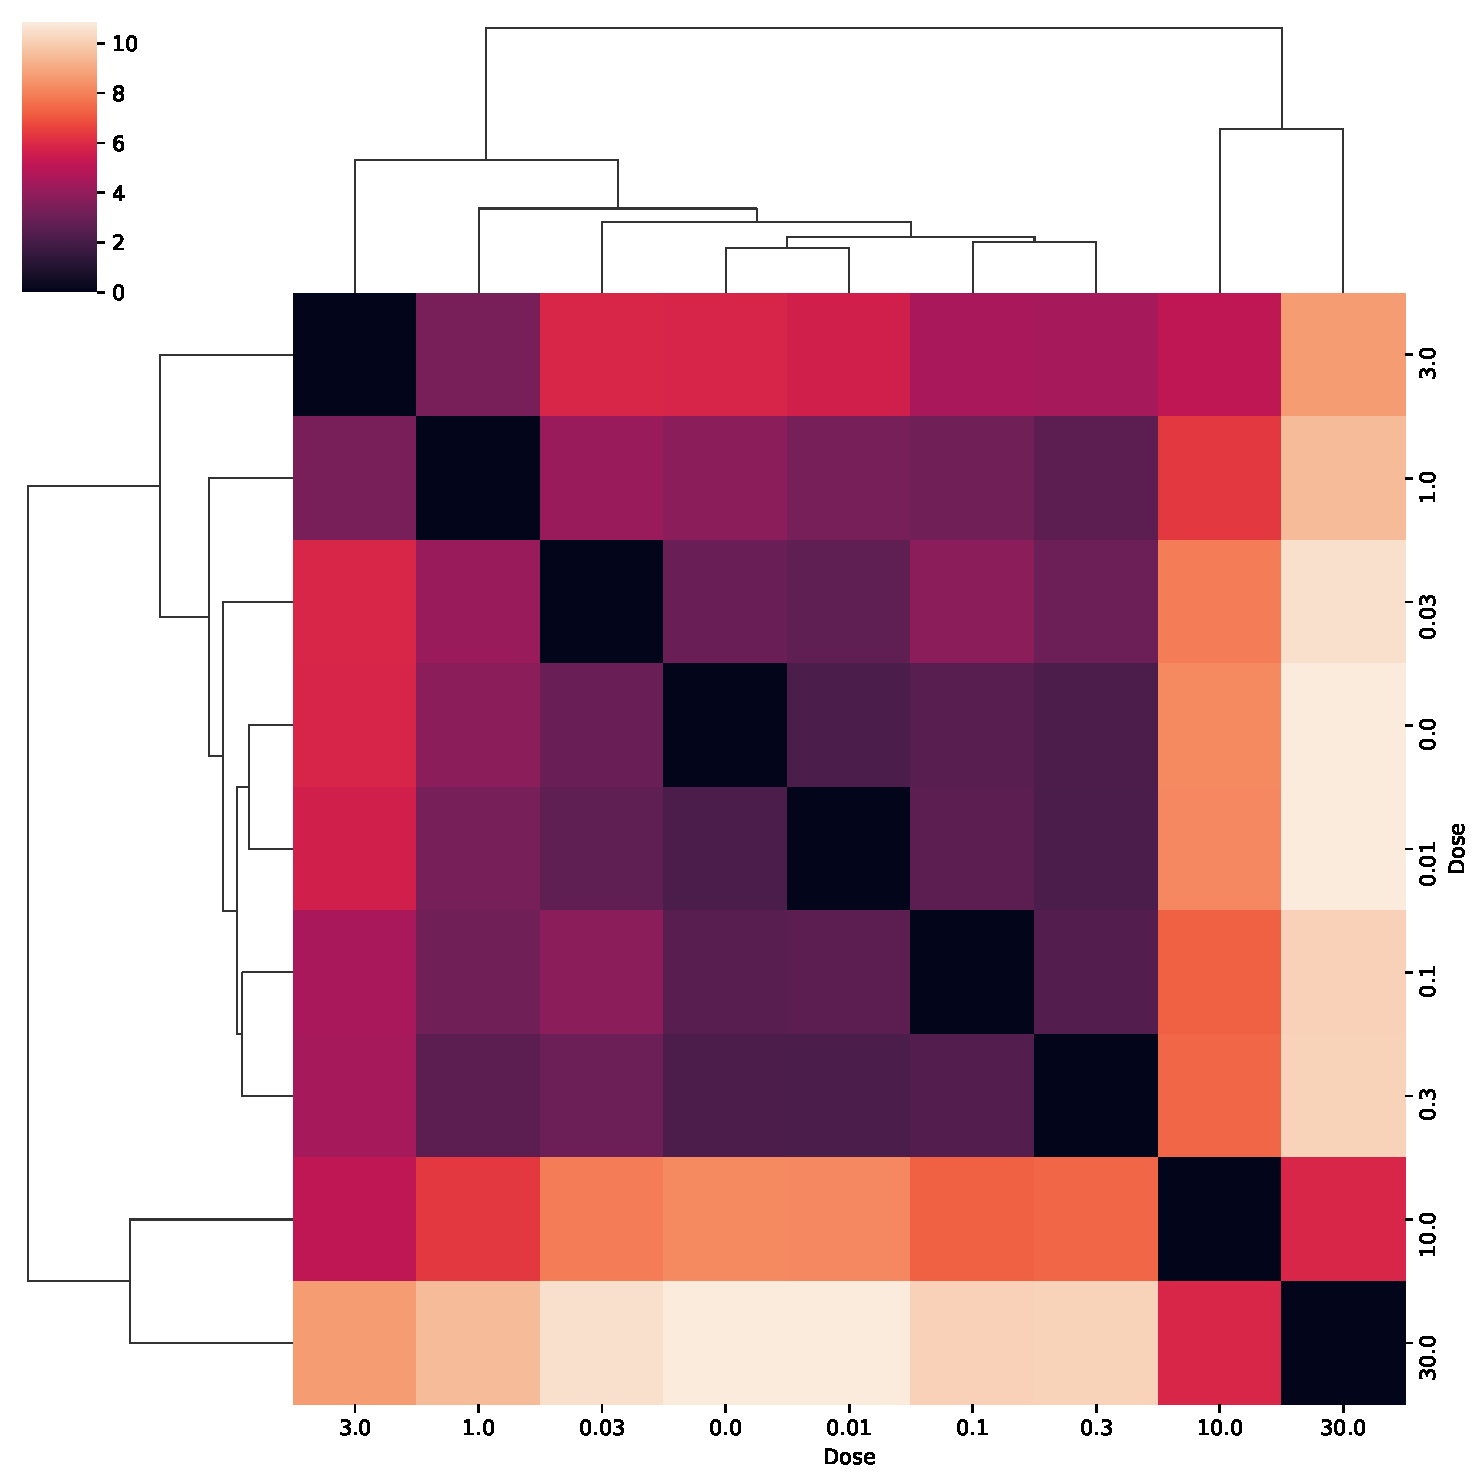
\includegraphics[width=\textwidth]{figures/hepatocytes_euclidean_clustermap.pdf}
        \caption{Euclidean}
    \end{minipage}
    \vskip\baselineskip

    \begin{minipage}{0.4\textwidth}
        \centering
        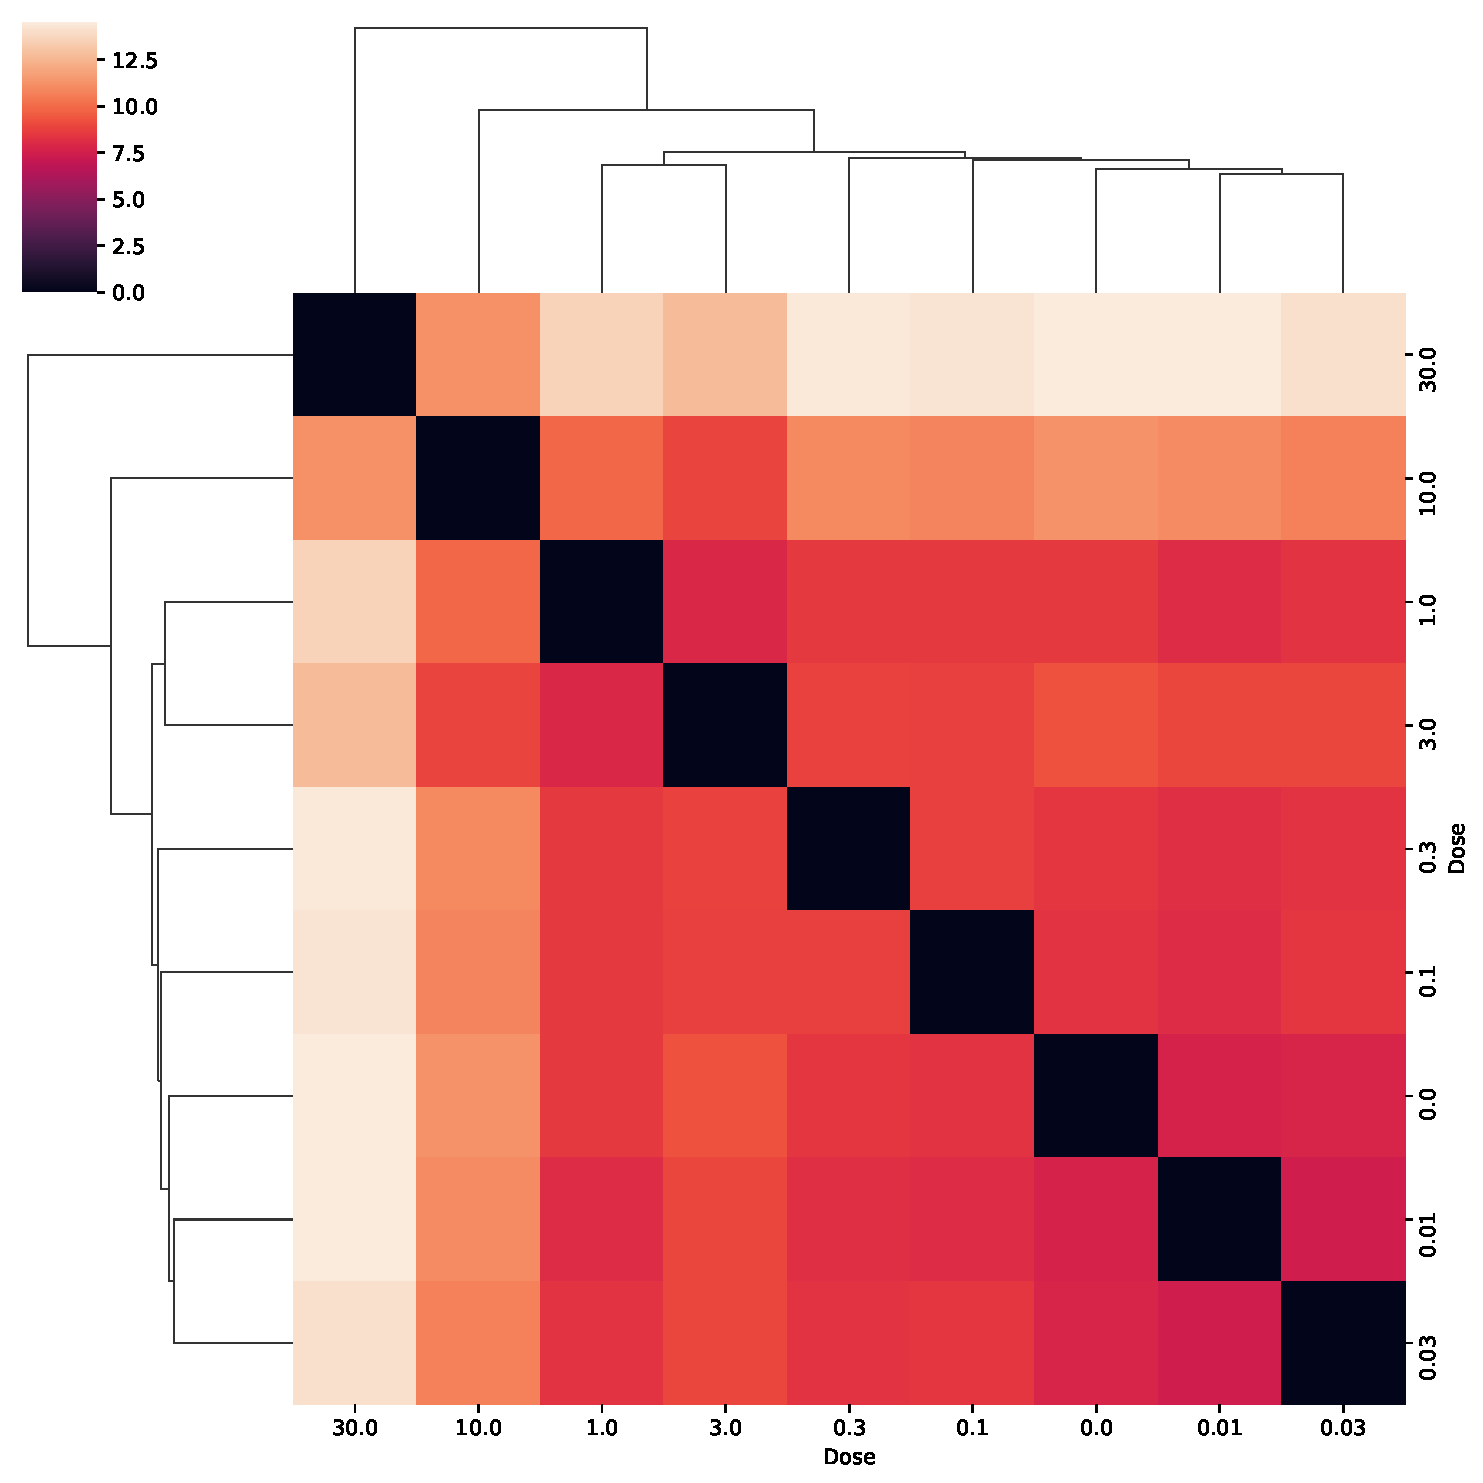
\includegraphics[width=\textwidth]{figures/hepatocytes_mean_pairwise_clustermap.pdf}
        \caption{Mean pairwise}
    \end{minipage} \hfill
    \begin{minipage}{0.4\textwidth}
        \centering
        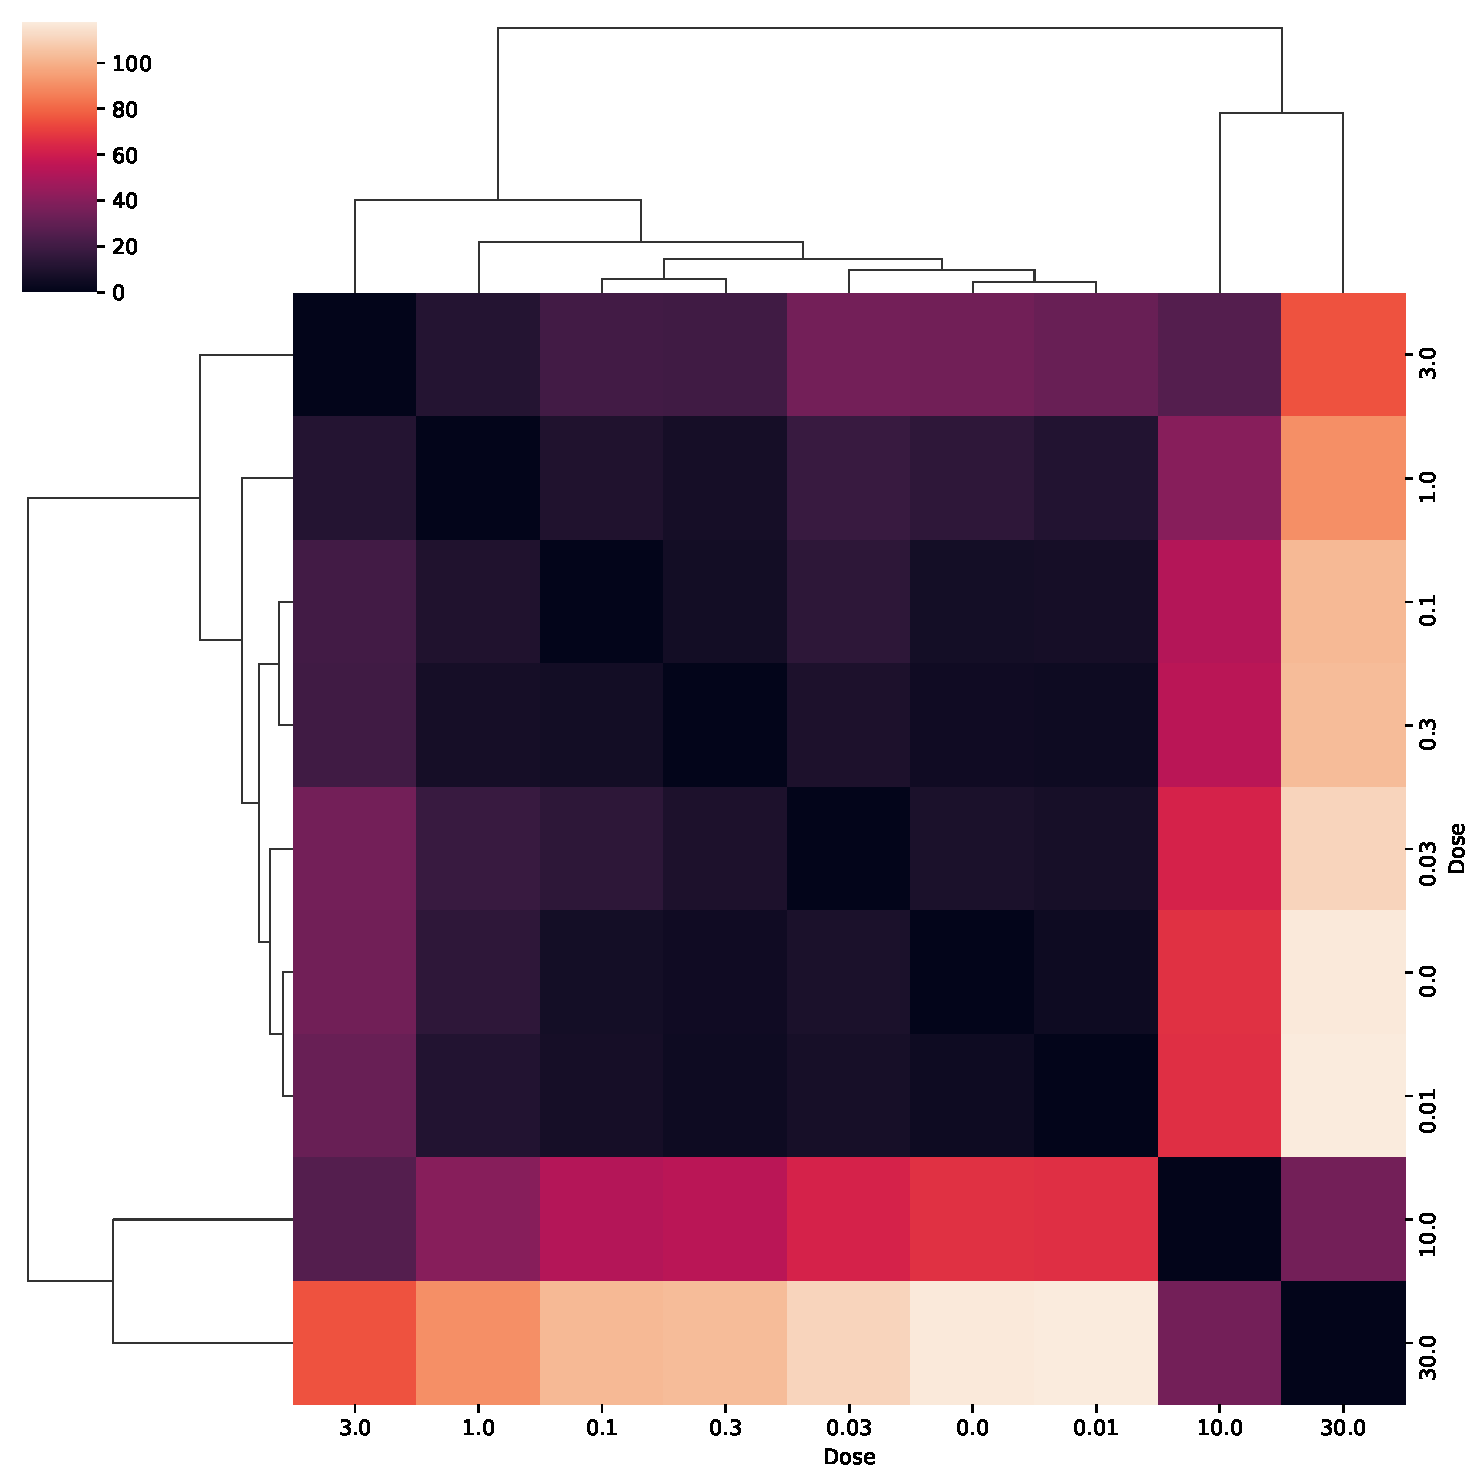
\includegraphics[width=\textwidth]{figures/hepatocytes_mmd_clustermap.pdf}
        \caption{MMD}
    \end{minipage}
    \vskip\baselineskip

    \begin{minipage}{0.4\textwidth}
        \centering
        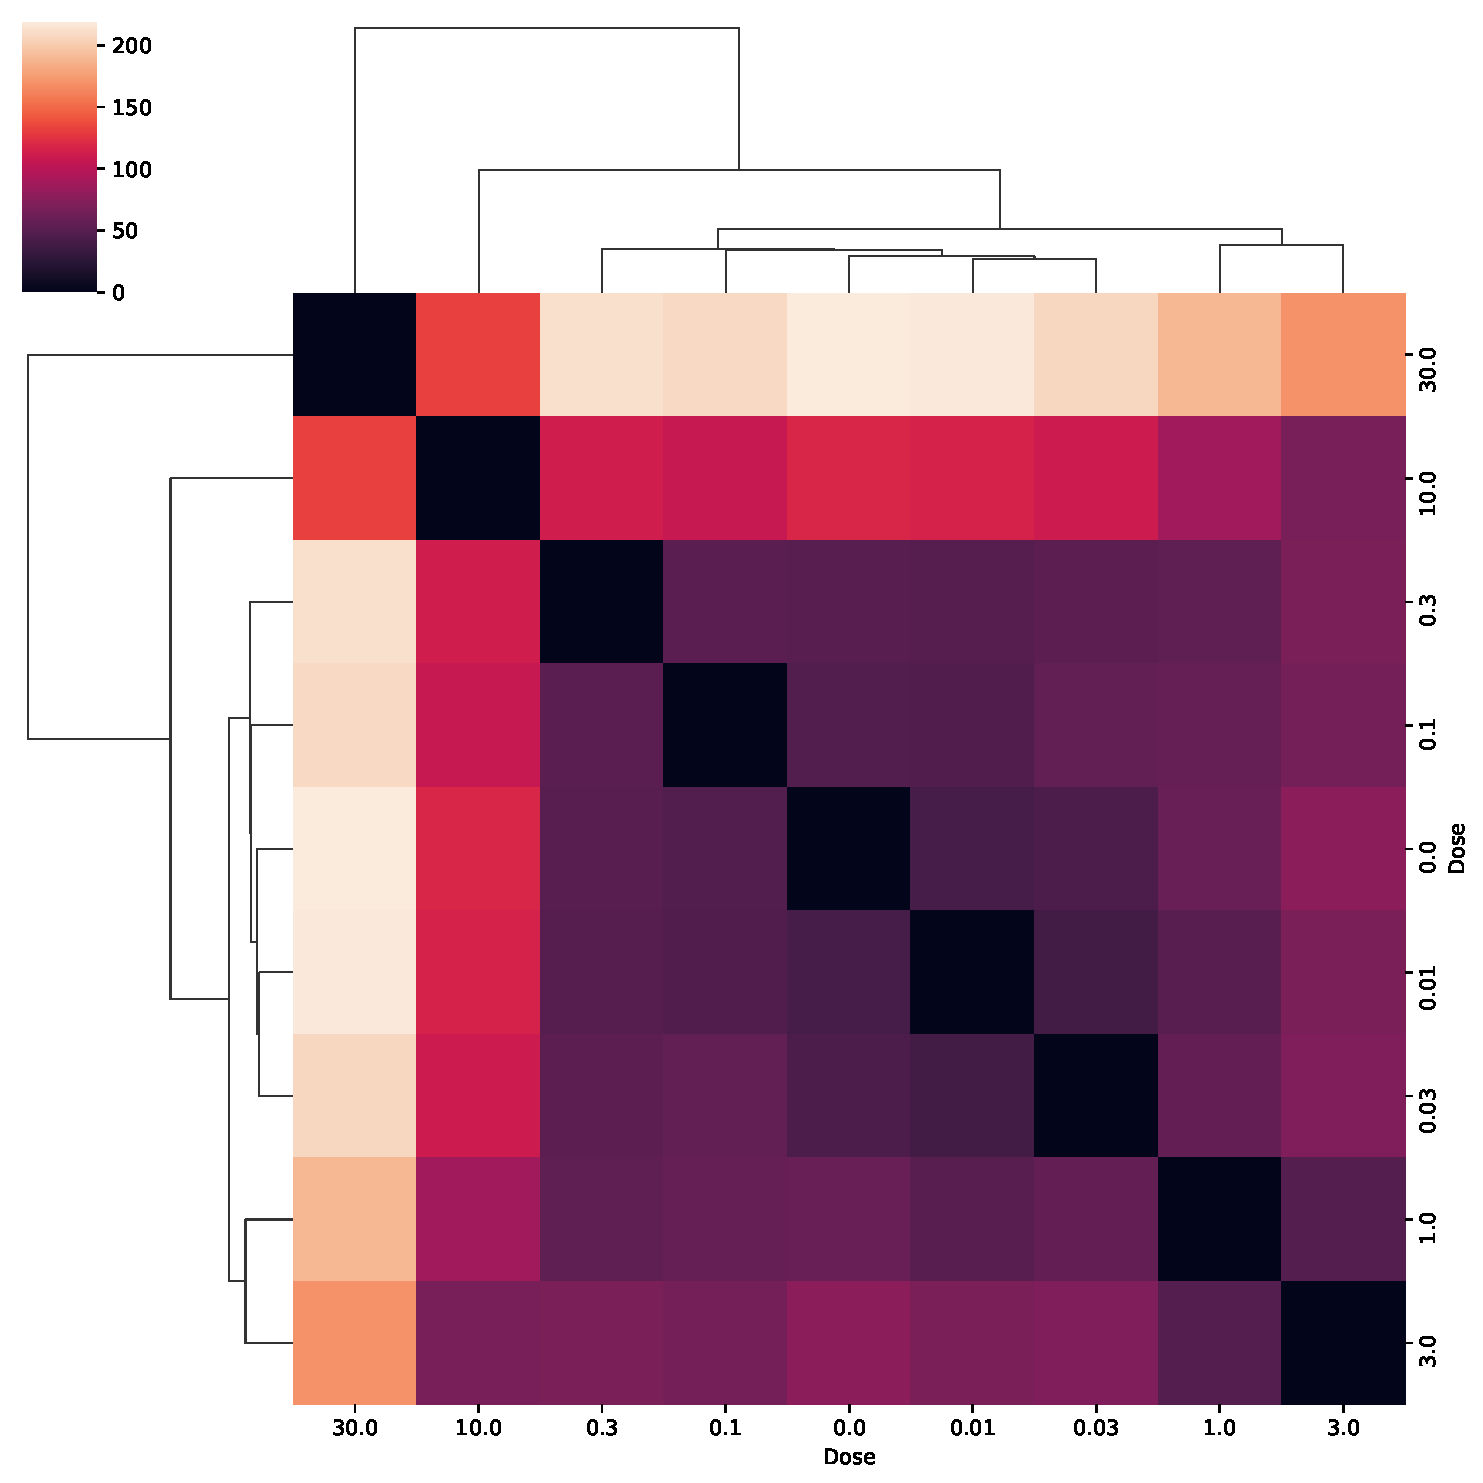
\includegraphics[width=\textwidth]{figures/hepatocytes_wasserstein_clustermap.pdf}
        \caption{Wasserstein}
    \end{minipage}
    \caption{Distance metrics for cell type Hepatocytes - portal per dosage}
\end{figure}

\begin{figure}
    \centering
    \begin{minipage}{0.4\textwidth}
        \centering
        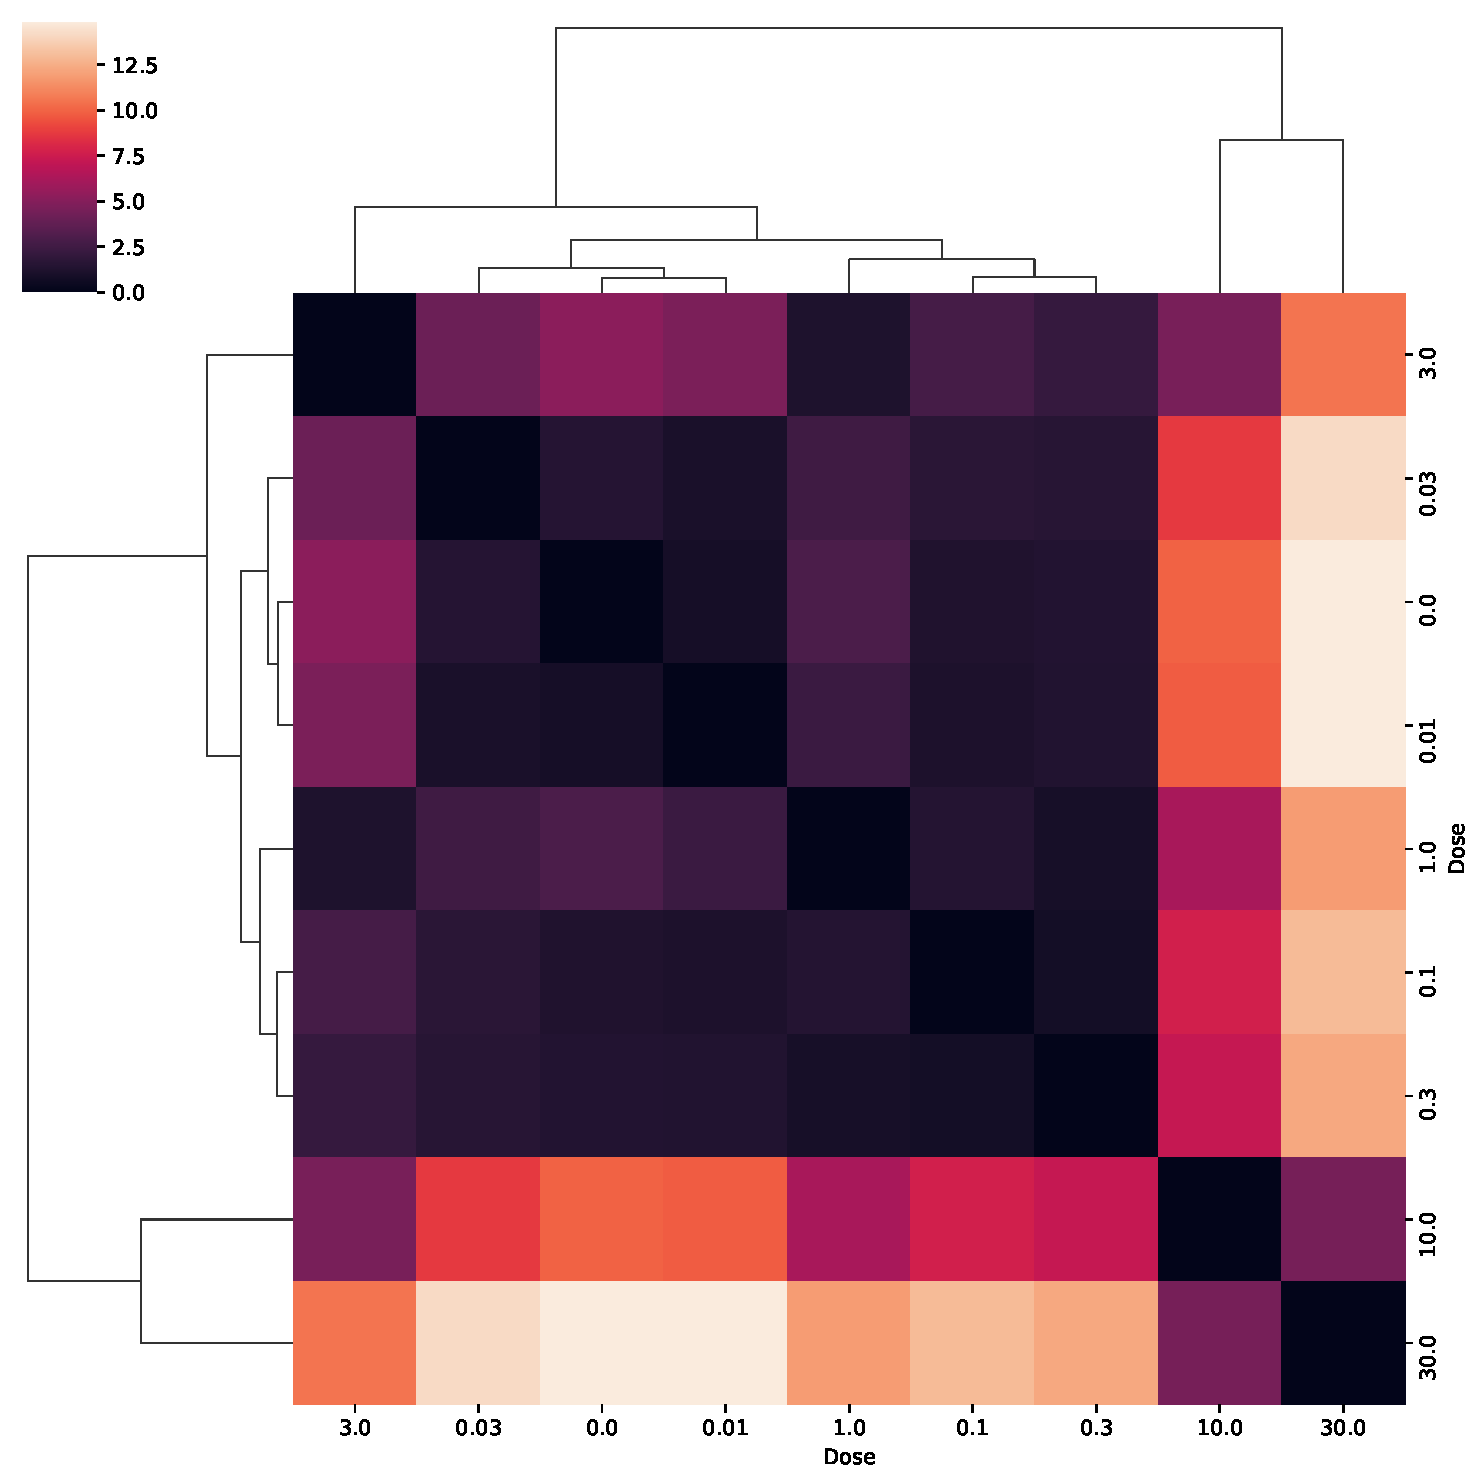
\includegraphics[width=\textwidth]{figures/hepatocytes_central_edistance_clustermap.pdf}
        \caption{E-distance}
    \end{minipage} \hfill
    \begin{minipage}{0.4\textwidth}
        \centering
        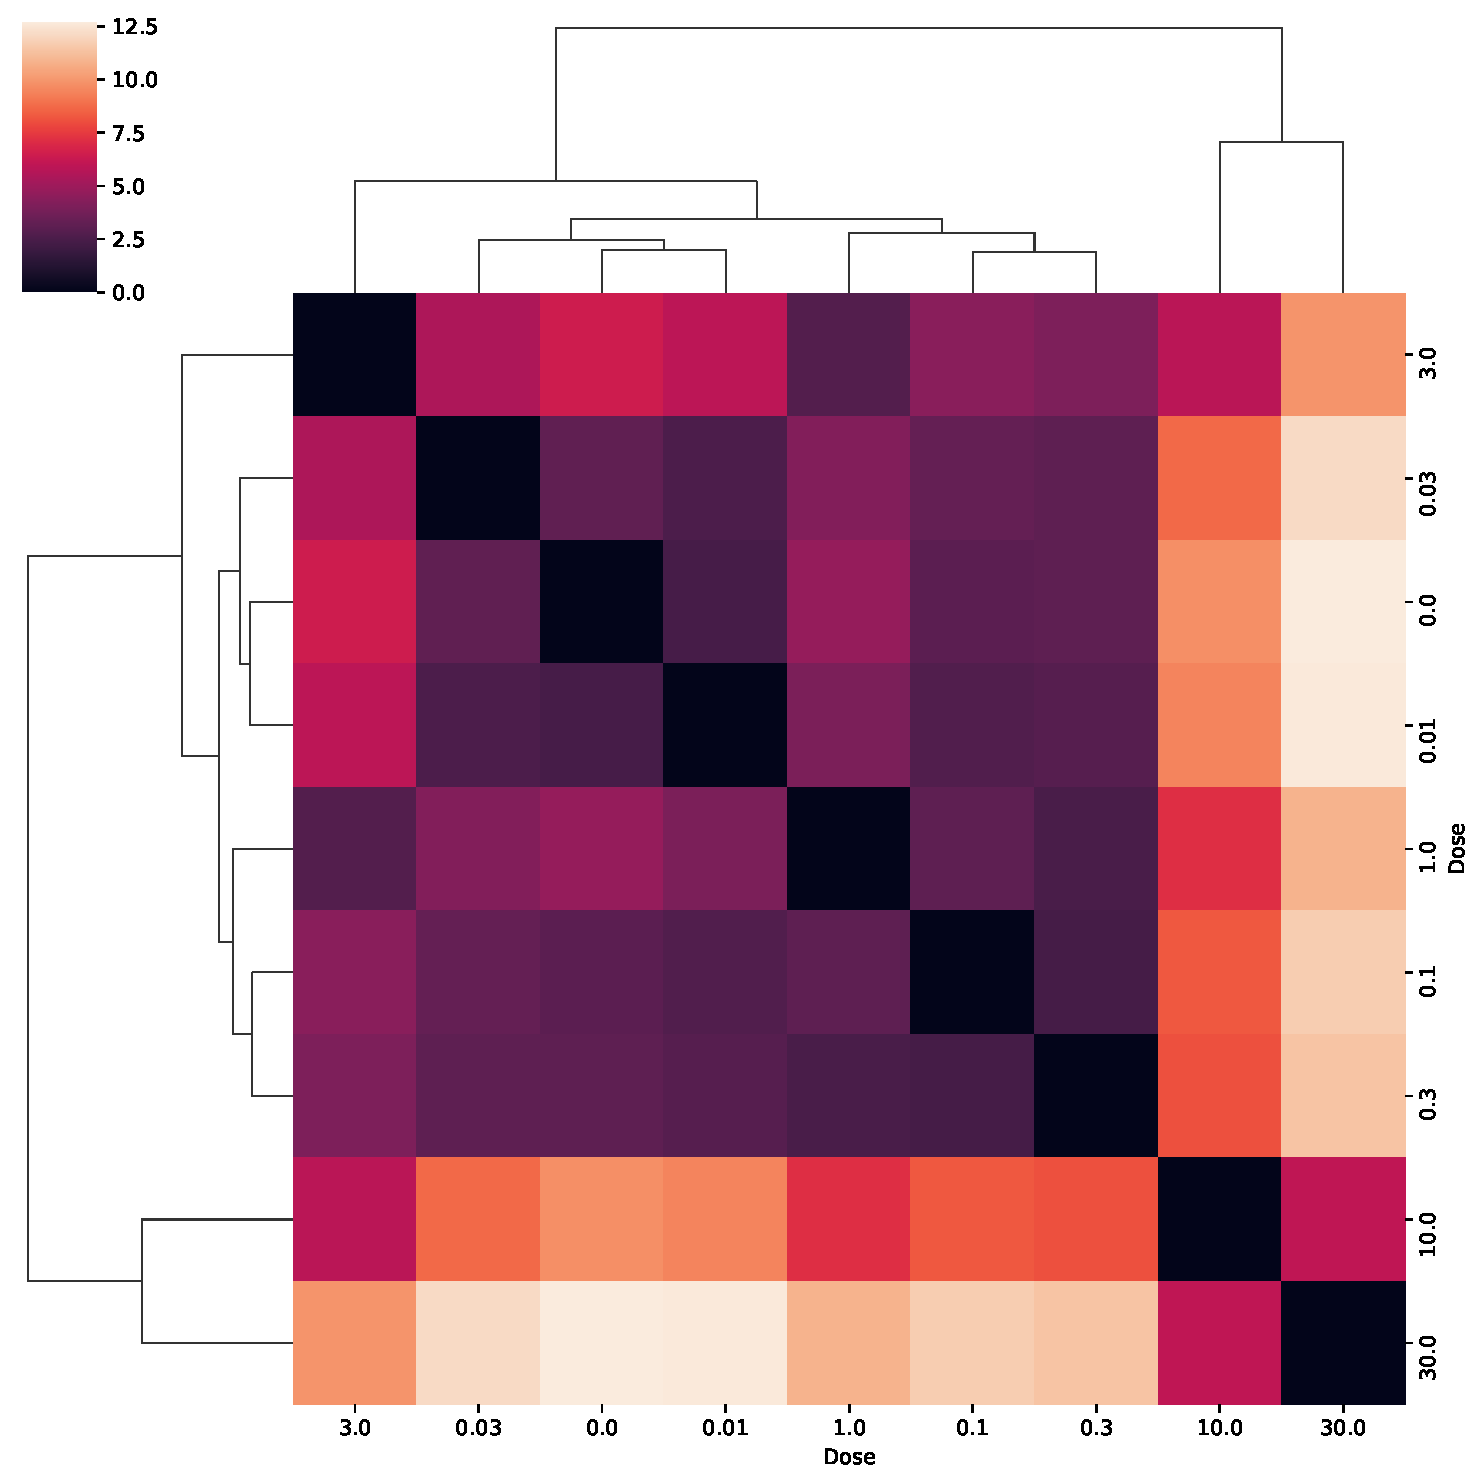
\includegraphics[width=\textwidth]{figures/hepatocytes_central_euclidean_clustermap.pdf}
        \caption{Euclidean}
    \end{minipage}
    \vskip\baselineskip

    \begin{minipage}{0.4\textwidth}
        \centering
        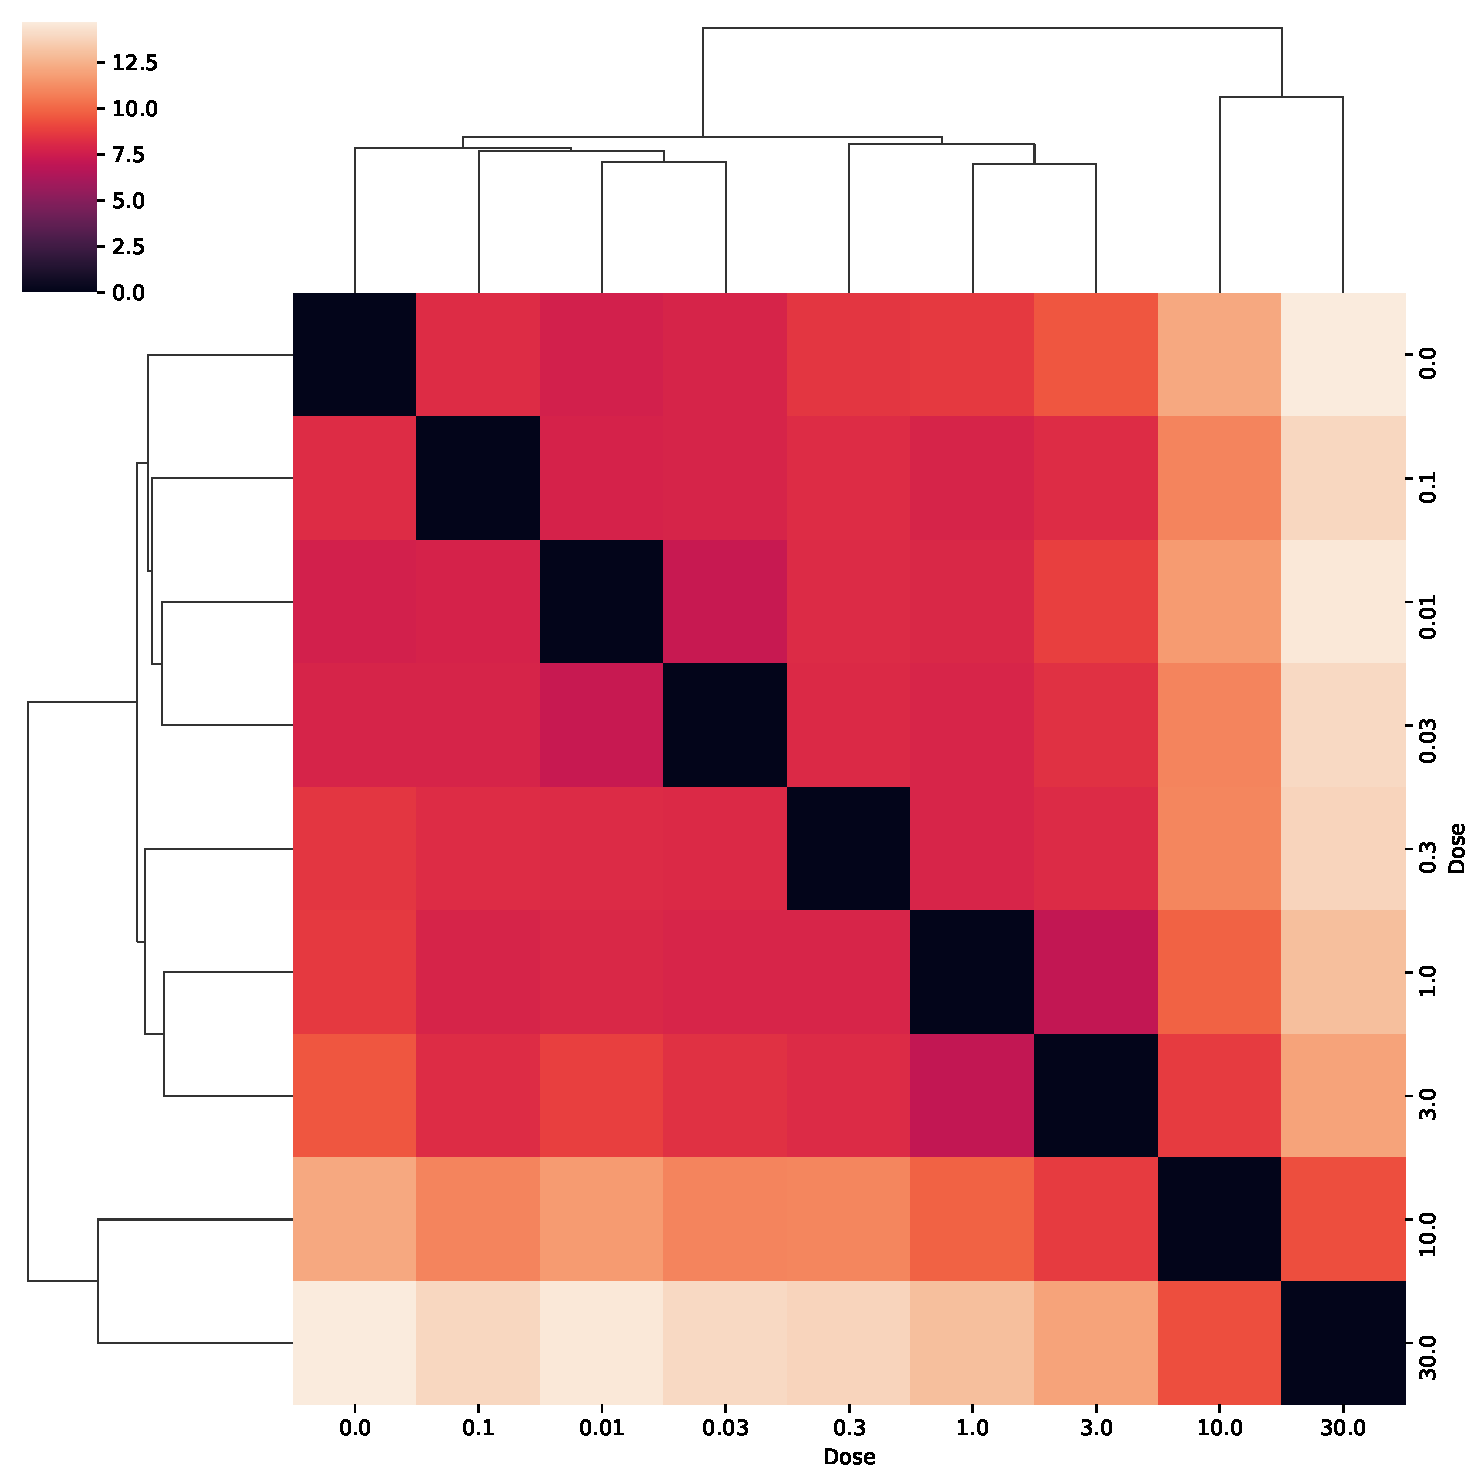
\includegraphics[width=\textwidth]{figures/hepatocytes_central_mean_pairwise_clustermap.pdf}
        \caption{Mean pairwise}
    \end{minipage} \hfill
    \begin{minipage}{0.4\textwidth}
        \centering
        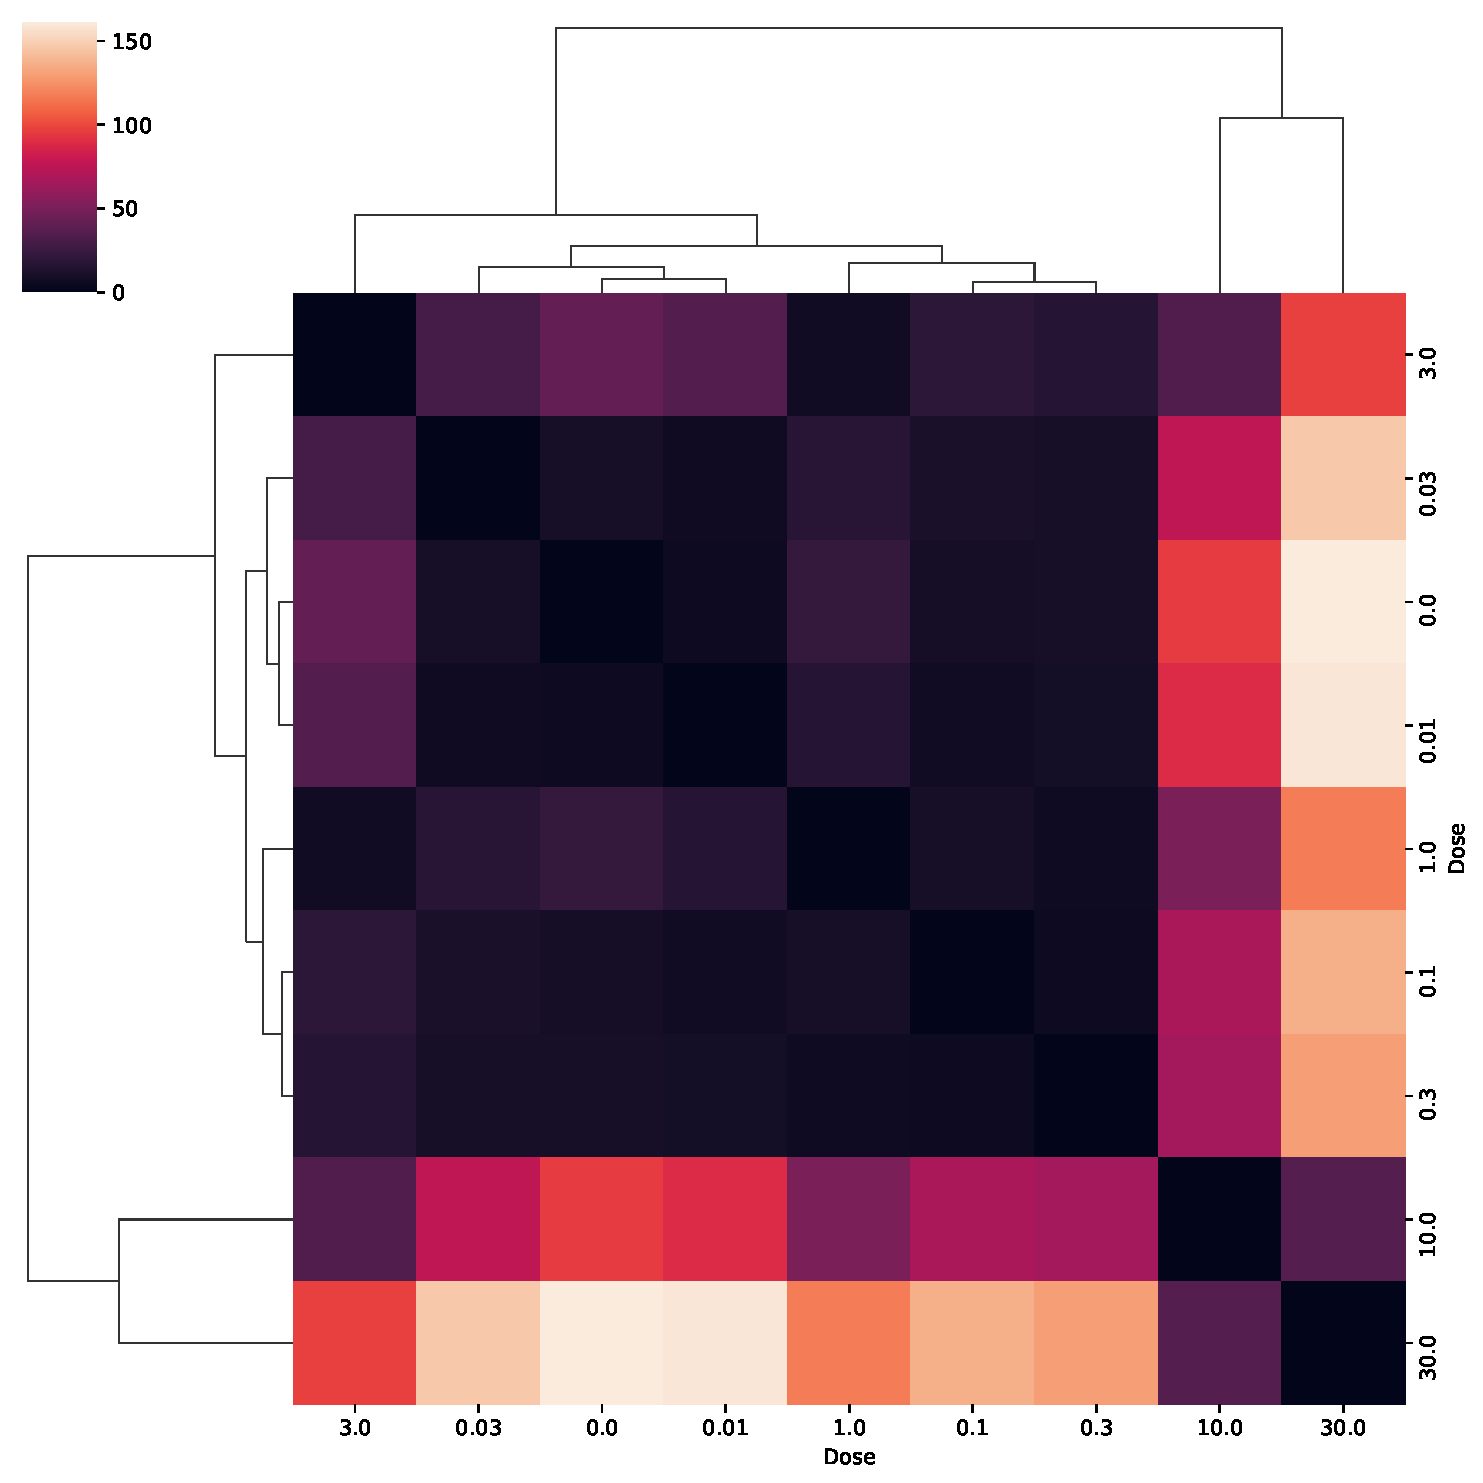
\includegraphics[width=\textwidth]{figures/hepatocytes_central_mmd_clustermap.pdf}
        \caption{MMD}
    \end{minipage}
    \vskip\baselineskip

    \begin{minipage}{0.4\textwidth}
        \centering
        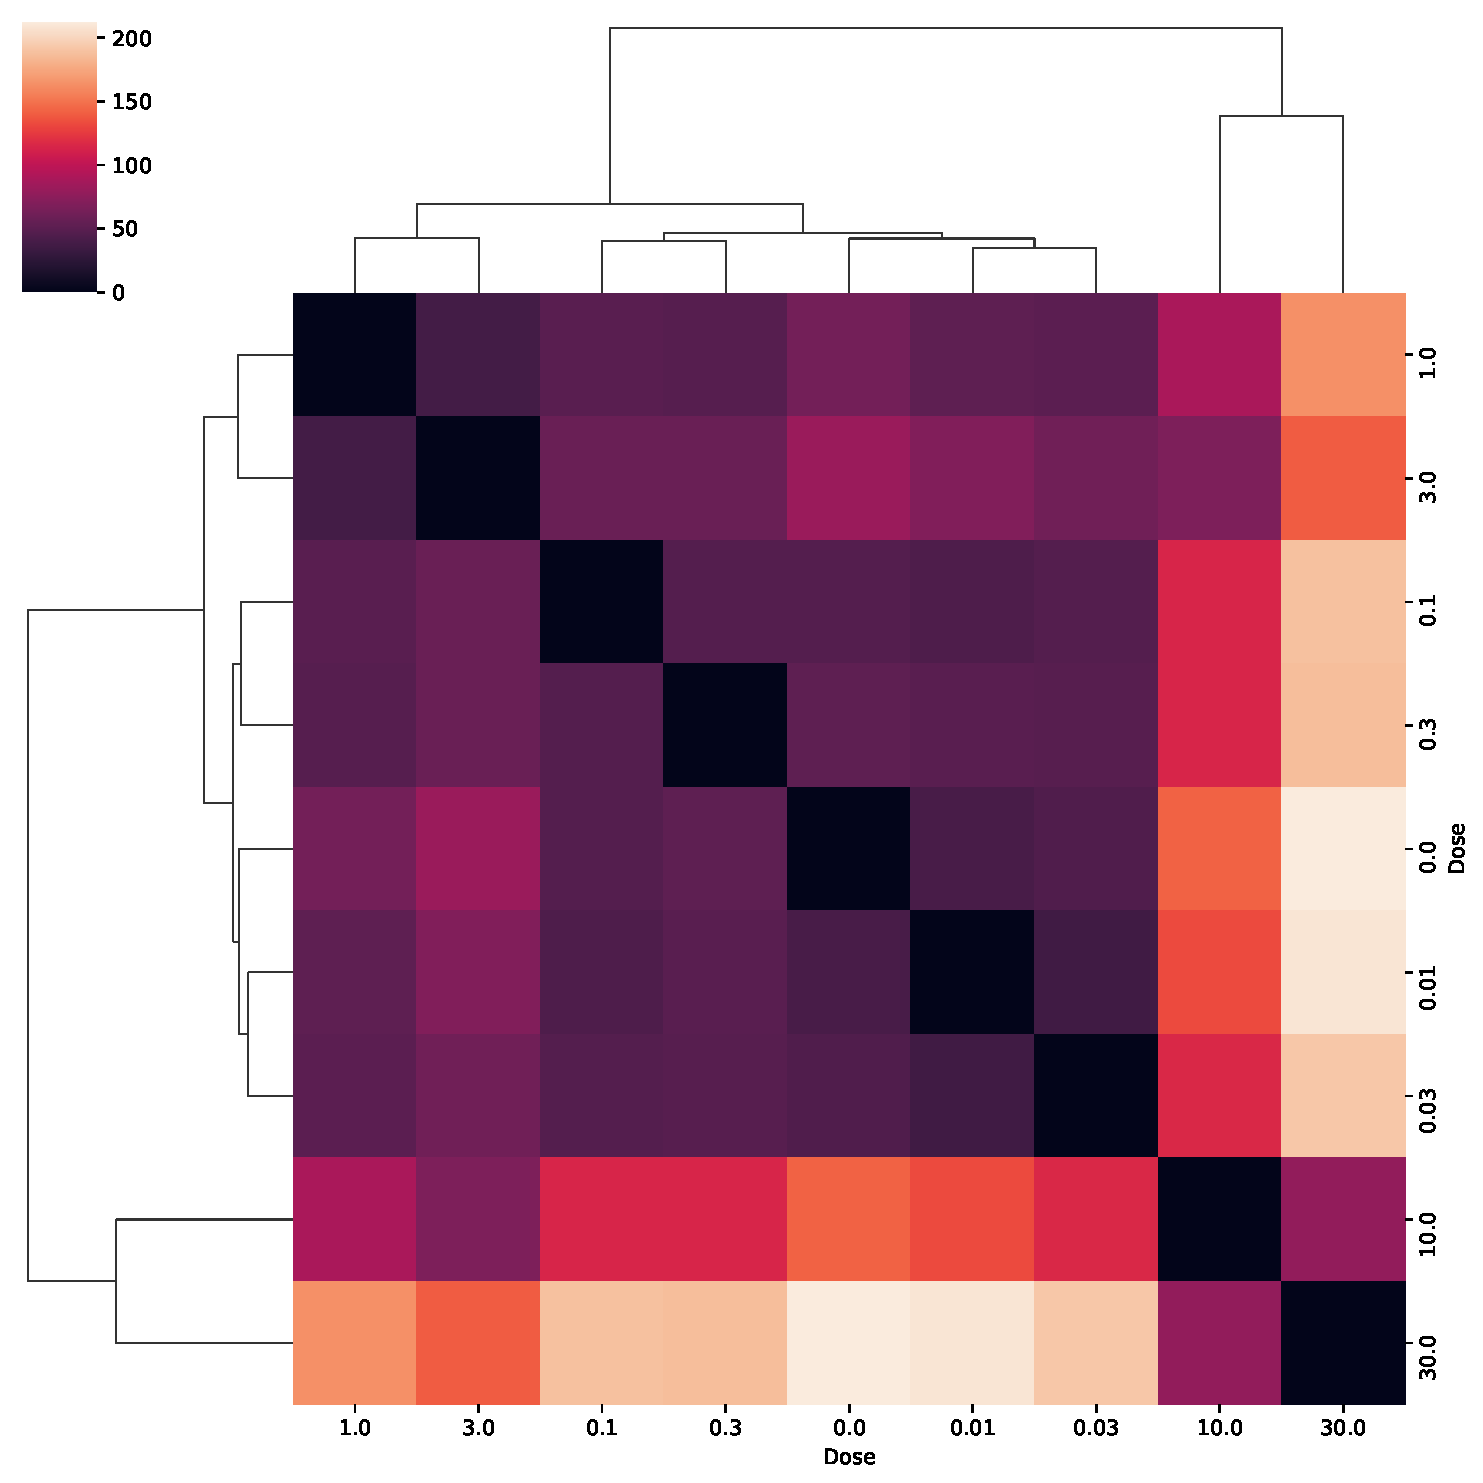
\includegraphics[width=\textwidth]{figures/hepatocytes_central_wasserstein_clustermap.pdf}
        \caption{Wasserstein}
    \end{minipage}
    \caption{Distance metrics for cell type Hepatocytes - central per dosage}
\end{figure}

\begin{figure}
    \centering
    \begin{minipage}{0.4\textwidth}
        \centering
        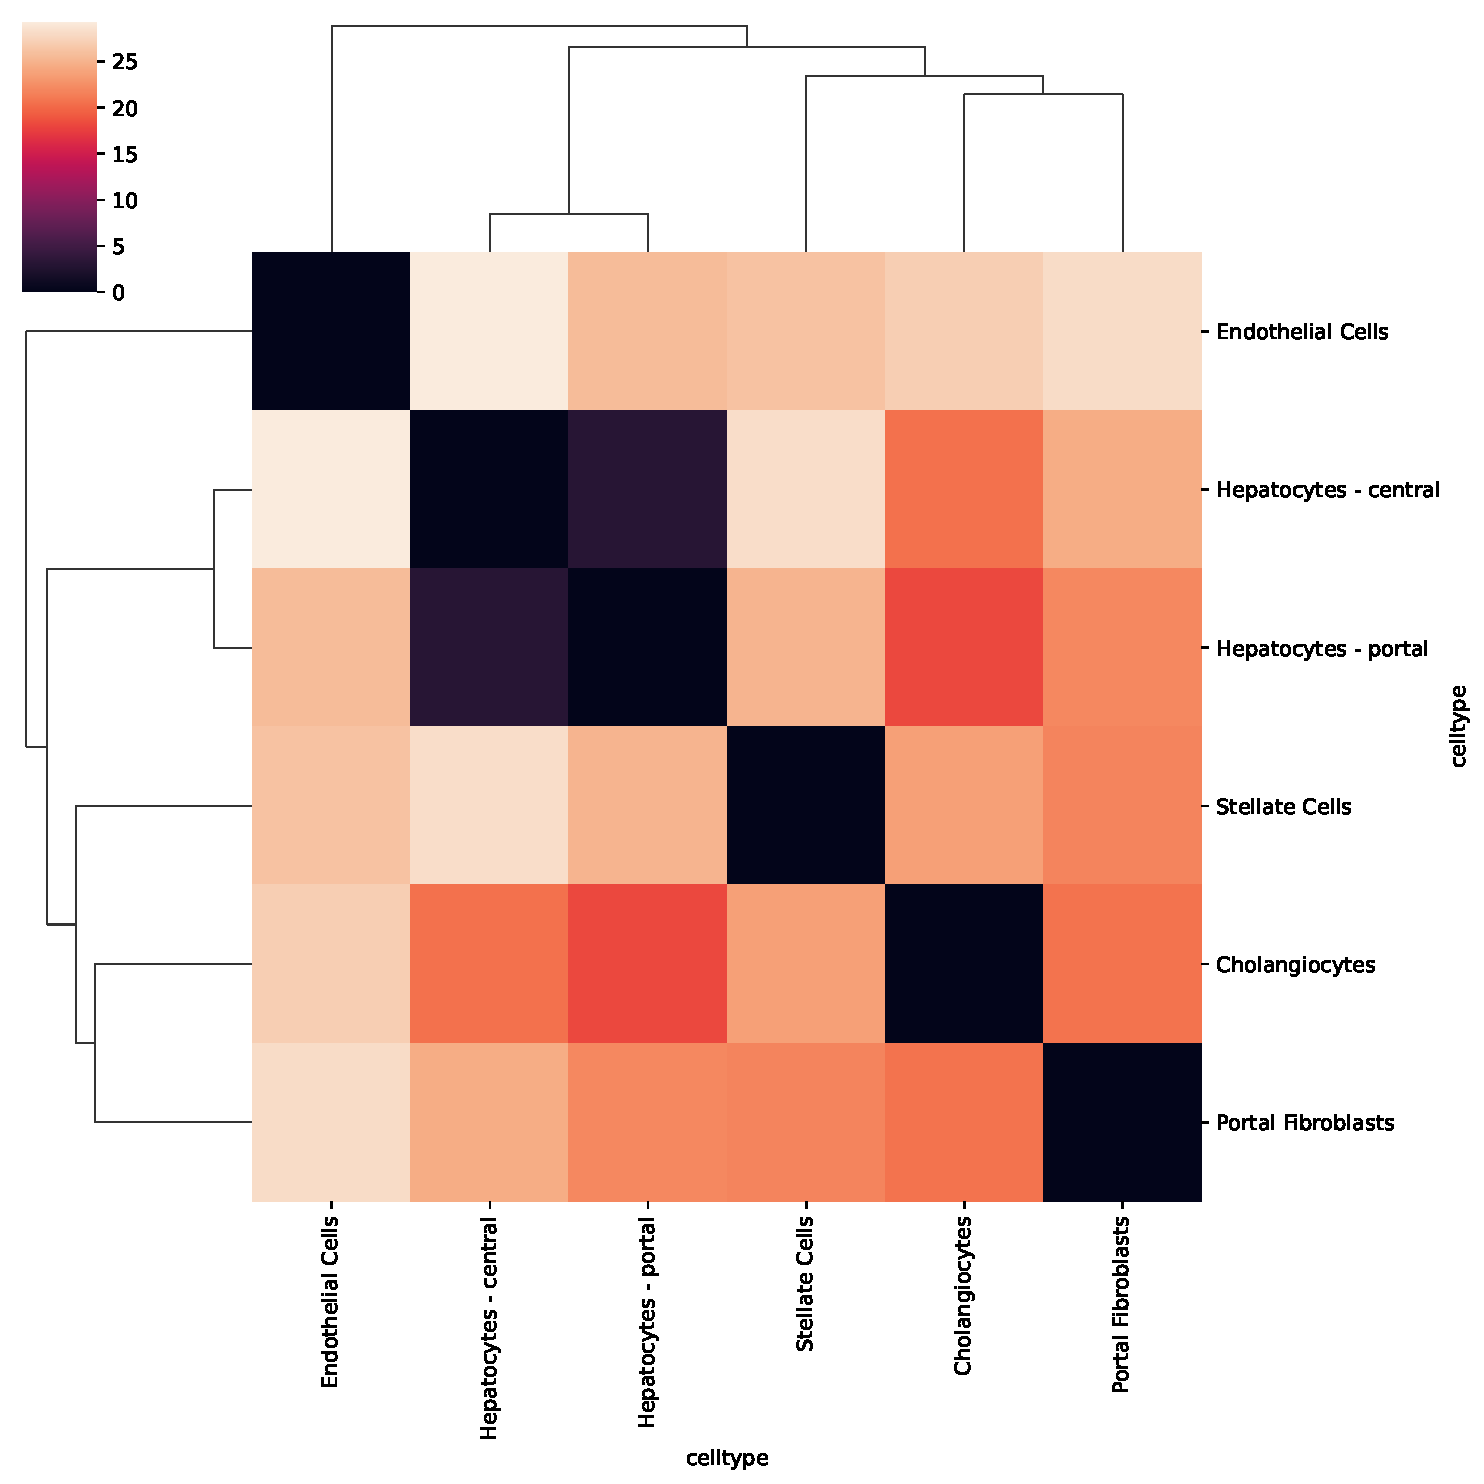
\includegraphics[width=\textwidth]{figures/dose_highest_edistance_clustermap.pdf}
        \caption{E-distance}
    \end{minipage} \hfill
    \begin{minipage}{0.4\textwidth}
        \centering
        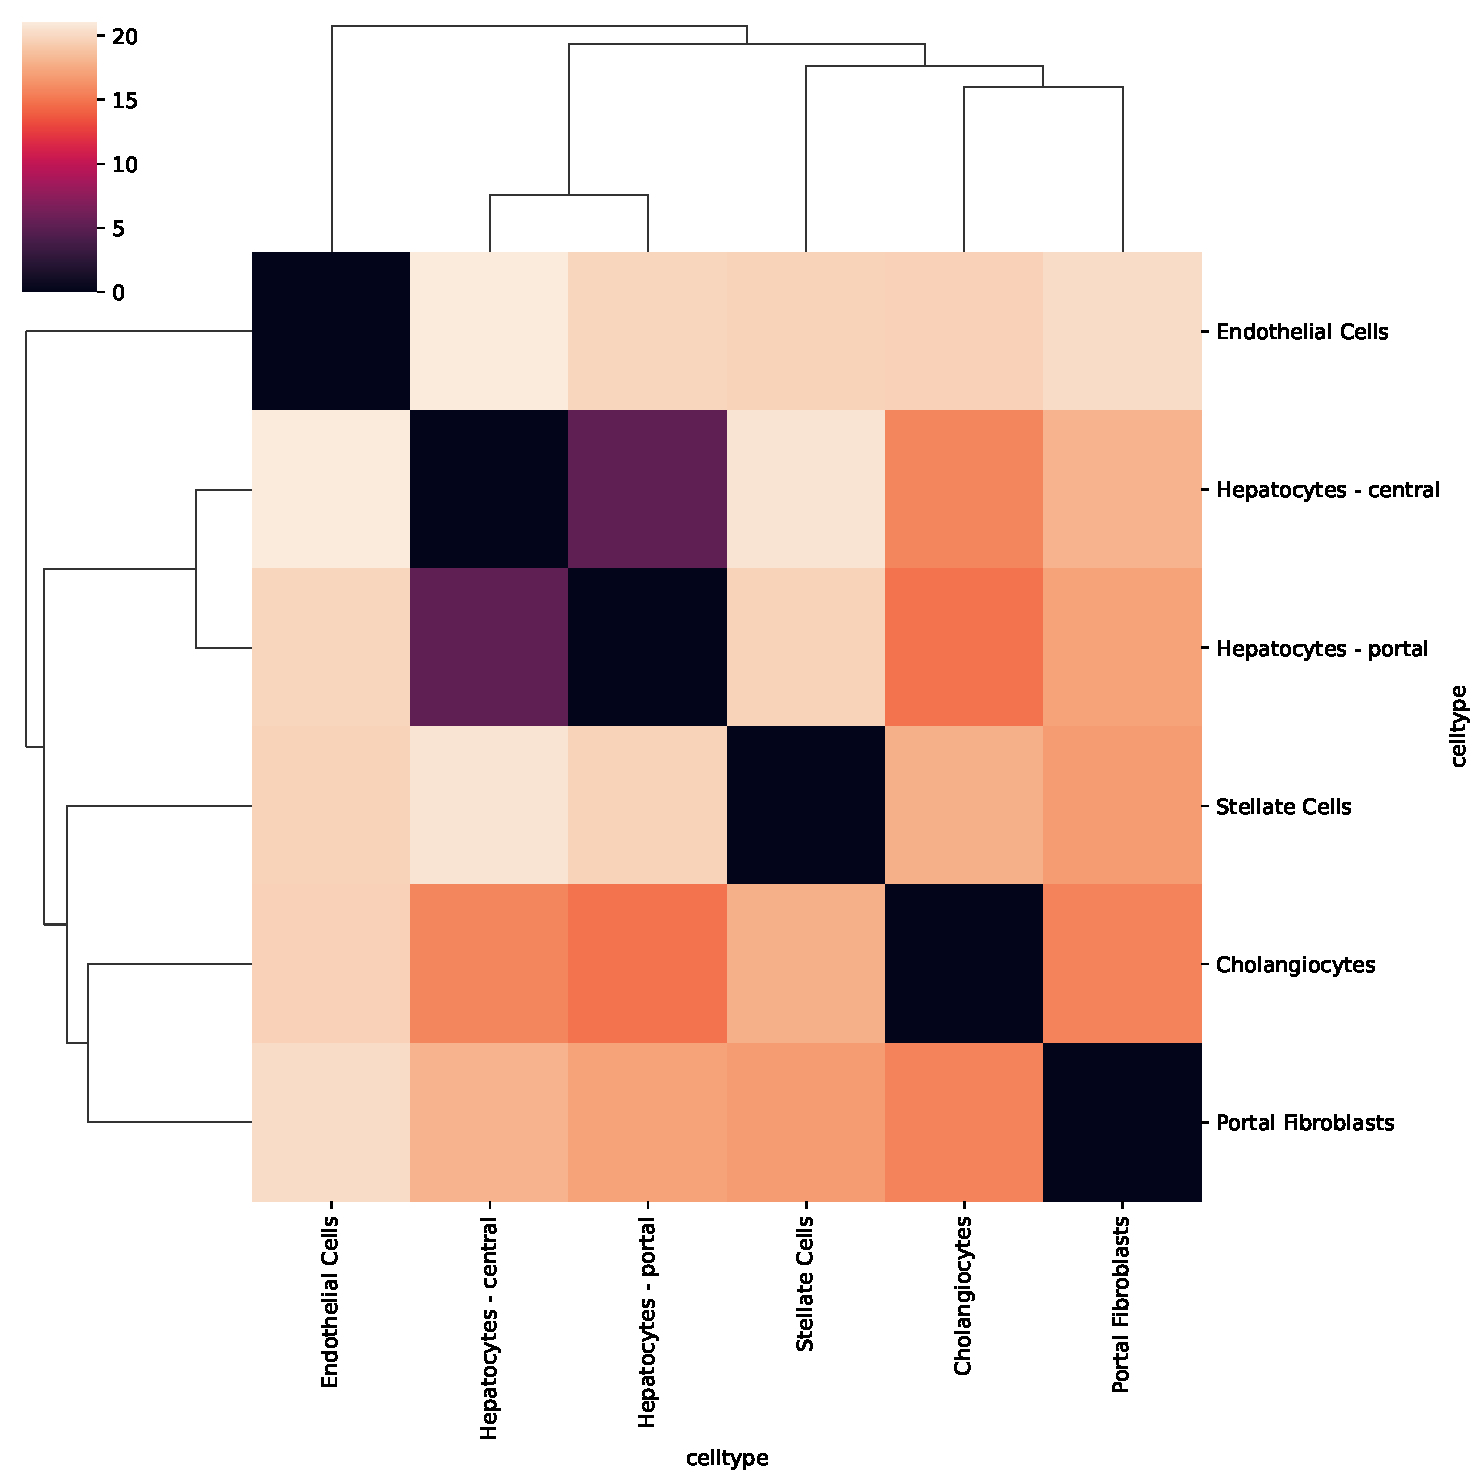
\includegraphics[width=\textwidth]{figures/dose_highest_euclidean_clustermap.pdf}
        \caption{Euclidean}
    \end{minipage}
    \vskip\baselineskip

    \begin{minipage}{0.4\textwidth}
        \centering
        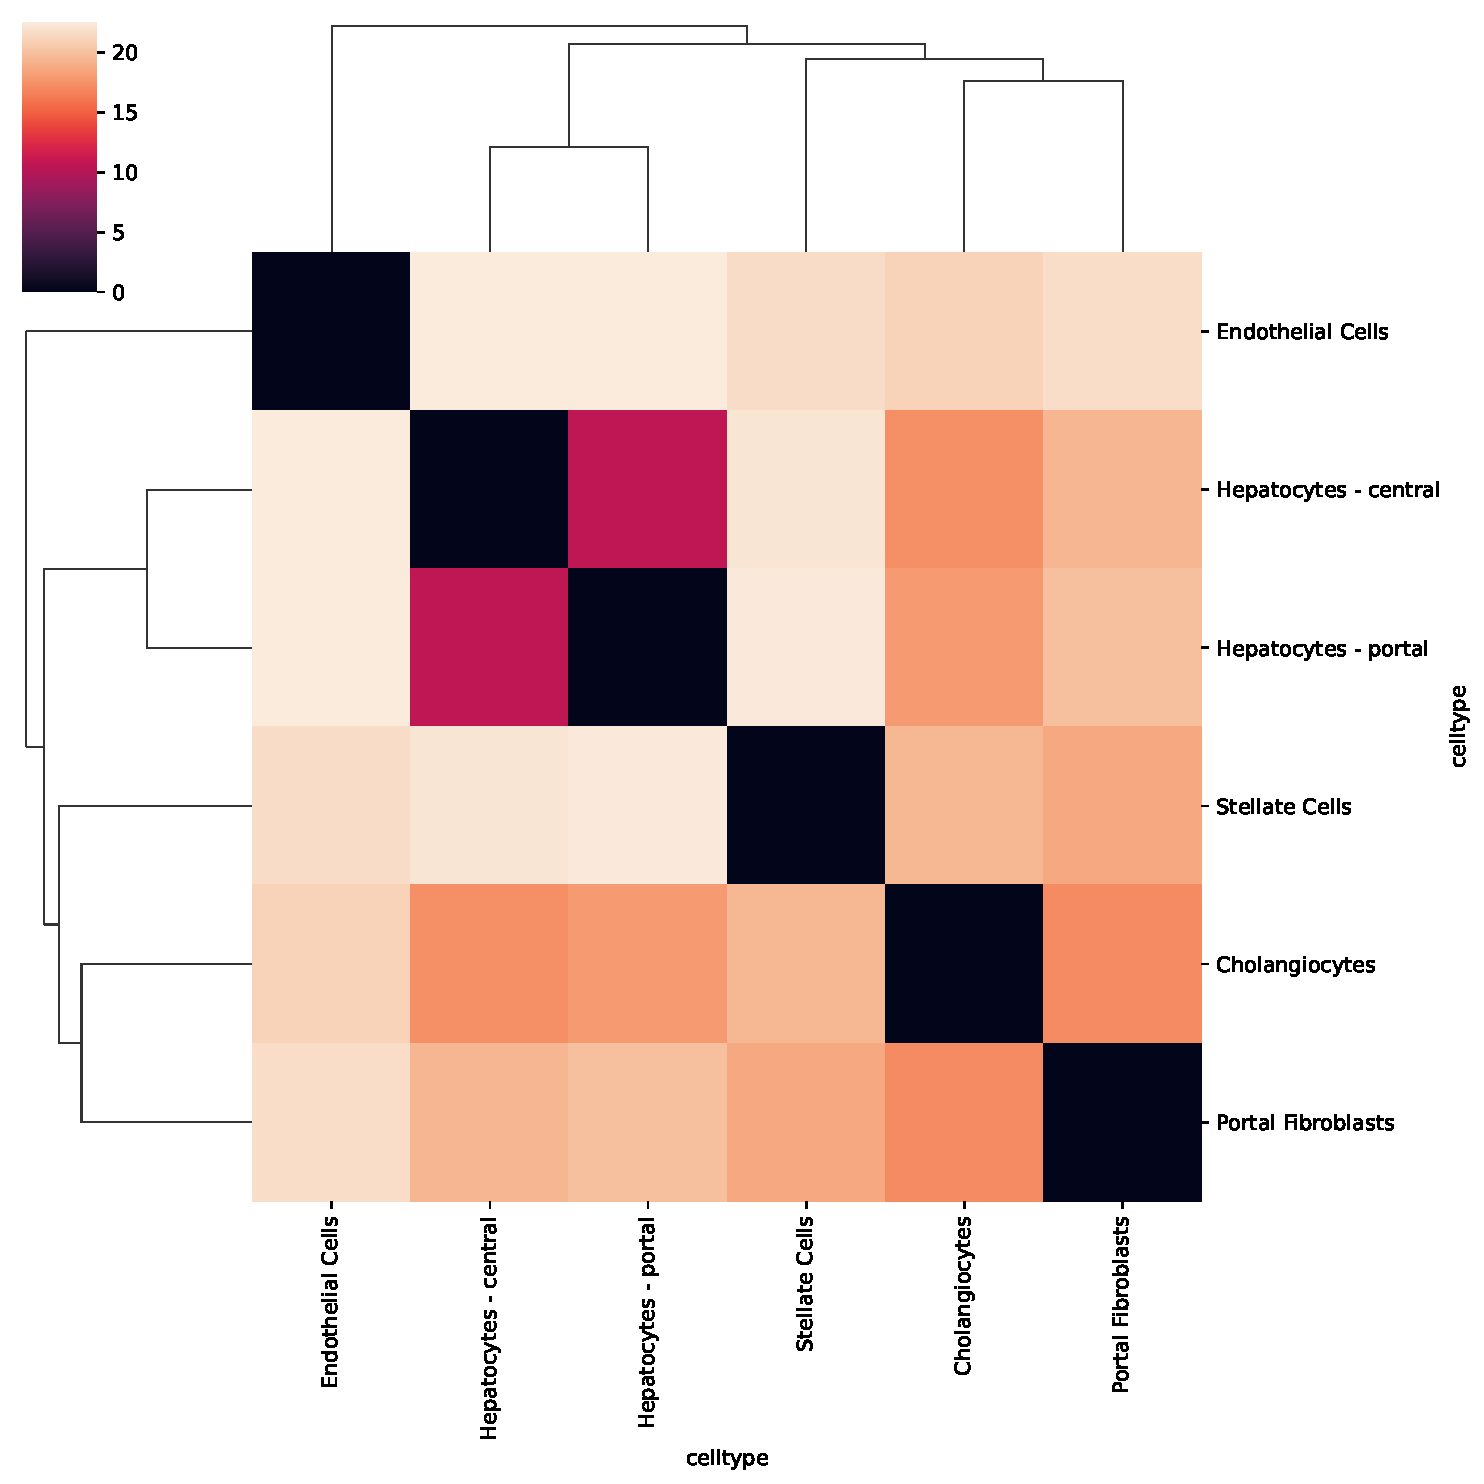
\includegraphics[width=\textwidth]{figures/dose_highest_mean_pairwise_clustermap.pdf}
        \caption{Mean pairwise}
    \end{minipage} \hfill
    \begin{minipage}{0.4\textwidth}
        \centering
        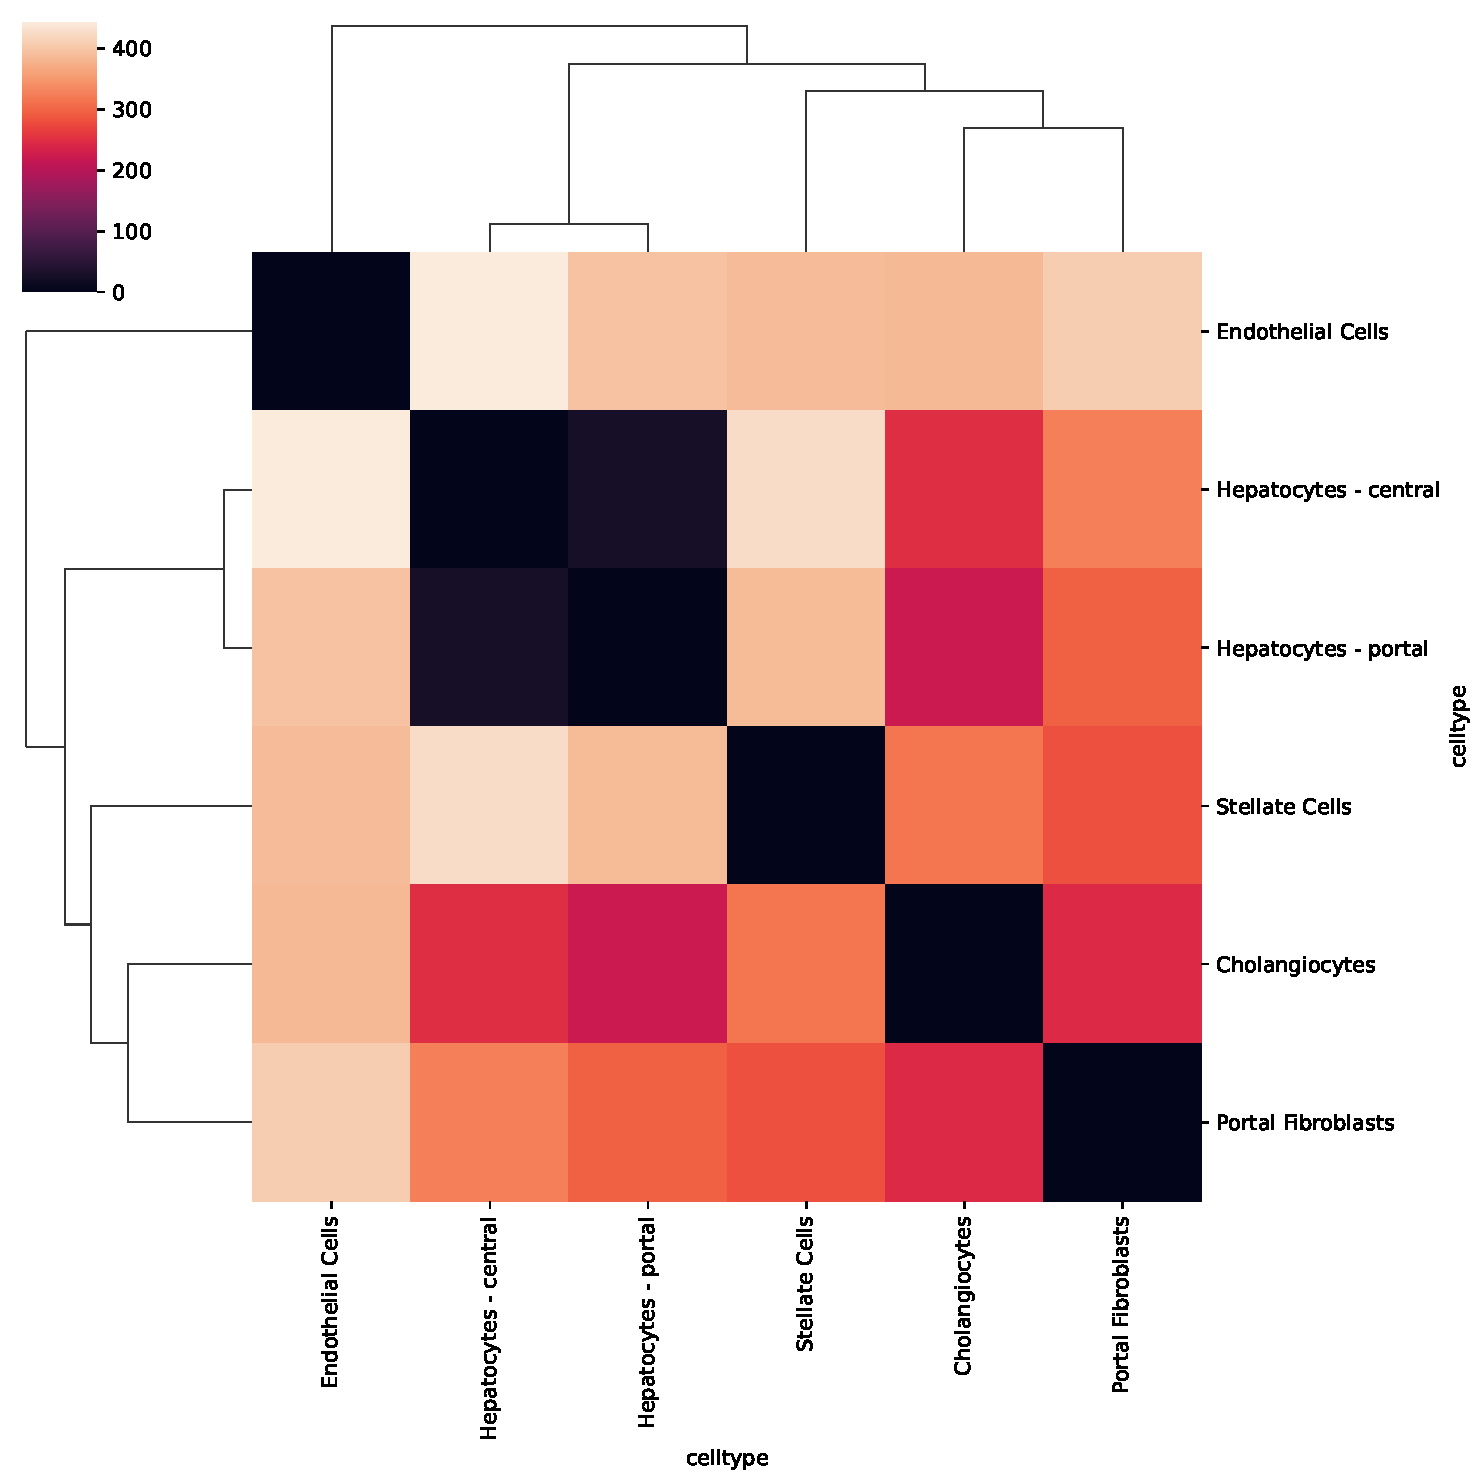
\includegraphics[width=\textwidth]{figures/dose_highest_mmd_clustermap.pdf}
        \caption{MMD}
    \end{minipage}
    \vskip\baselineskip

    \begin{minipage}{0.4\textwidth}
        \centering
        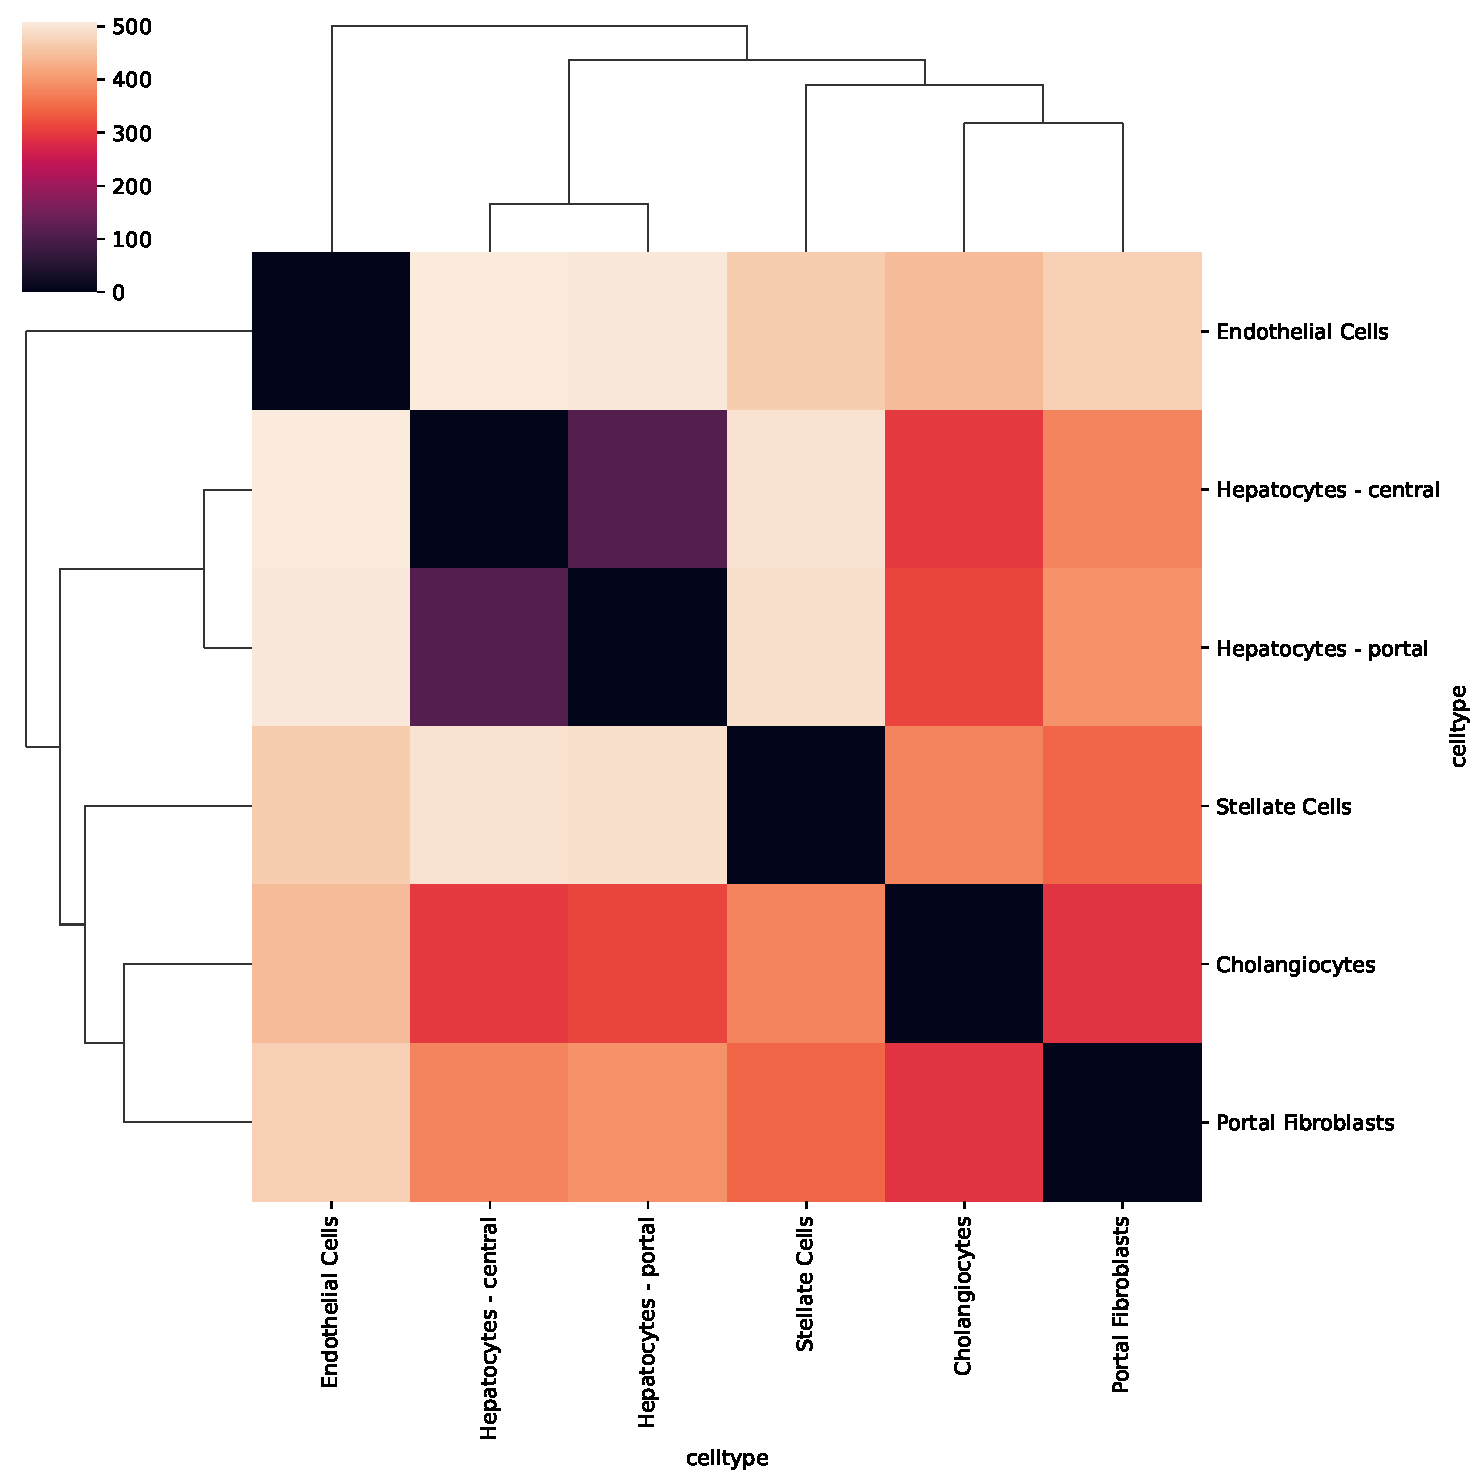
\includegraphics[width=\textwidth]{figures/dose_highest_wasserstein_clustermap.pdf}
        \caption{Wasserstein}
    \end{minipage}
    \caption{Distance metrics for dosage highest 30 $\mu g/kg$ per cell type}
\end{figure}

\begin{figure}
    \centering
    \begin{minipage}{0.4\textwidth}
        \centering
        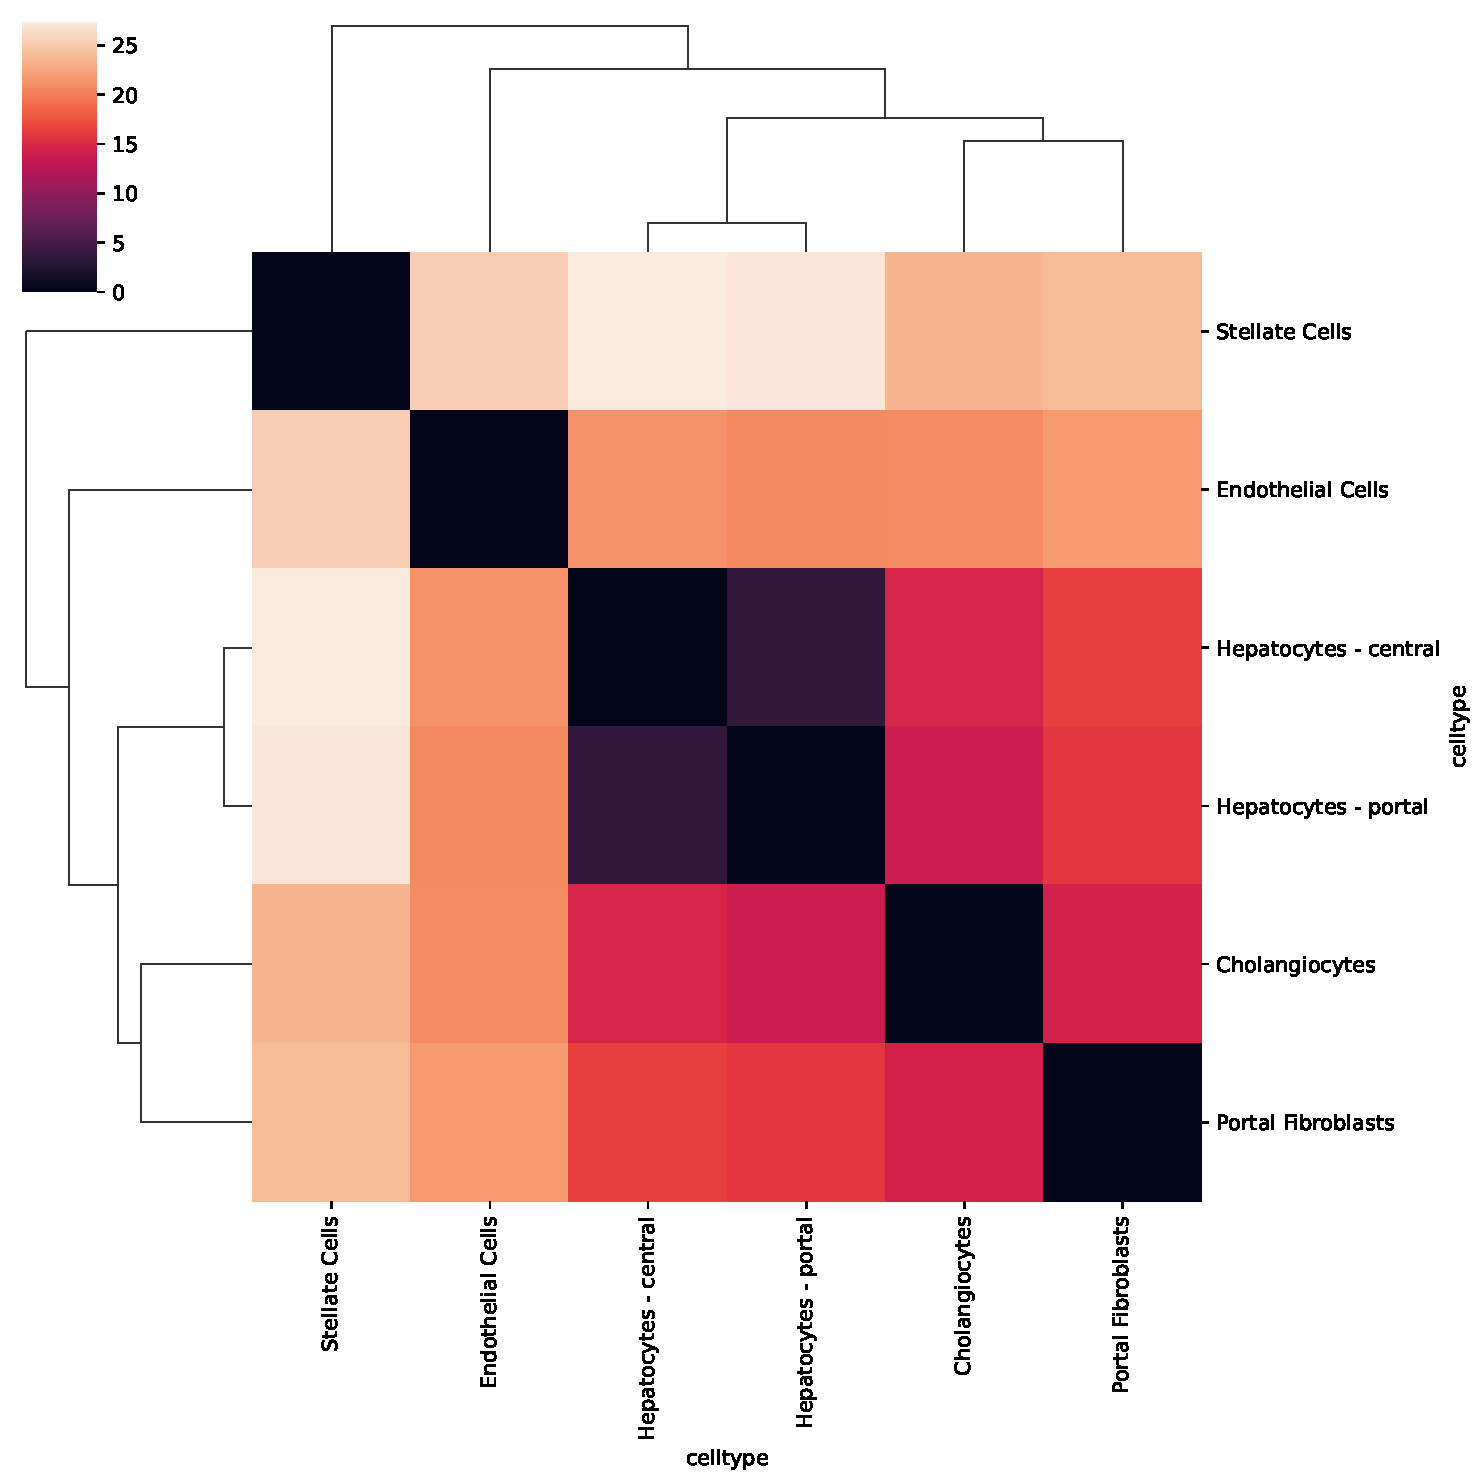
\includegraphics[width=\textwidth]{figures/dose_lowest_edistance_clustermap.pdf}
        \caption{E-distance}
    \end{minipage} \hfill
    \begin{minipage}{0.4\textwidth}
        \centering
        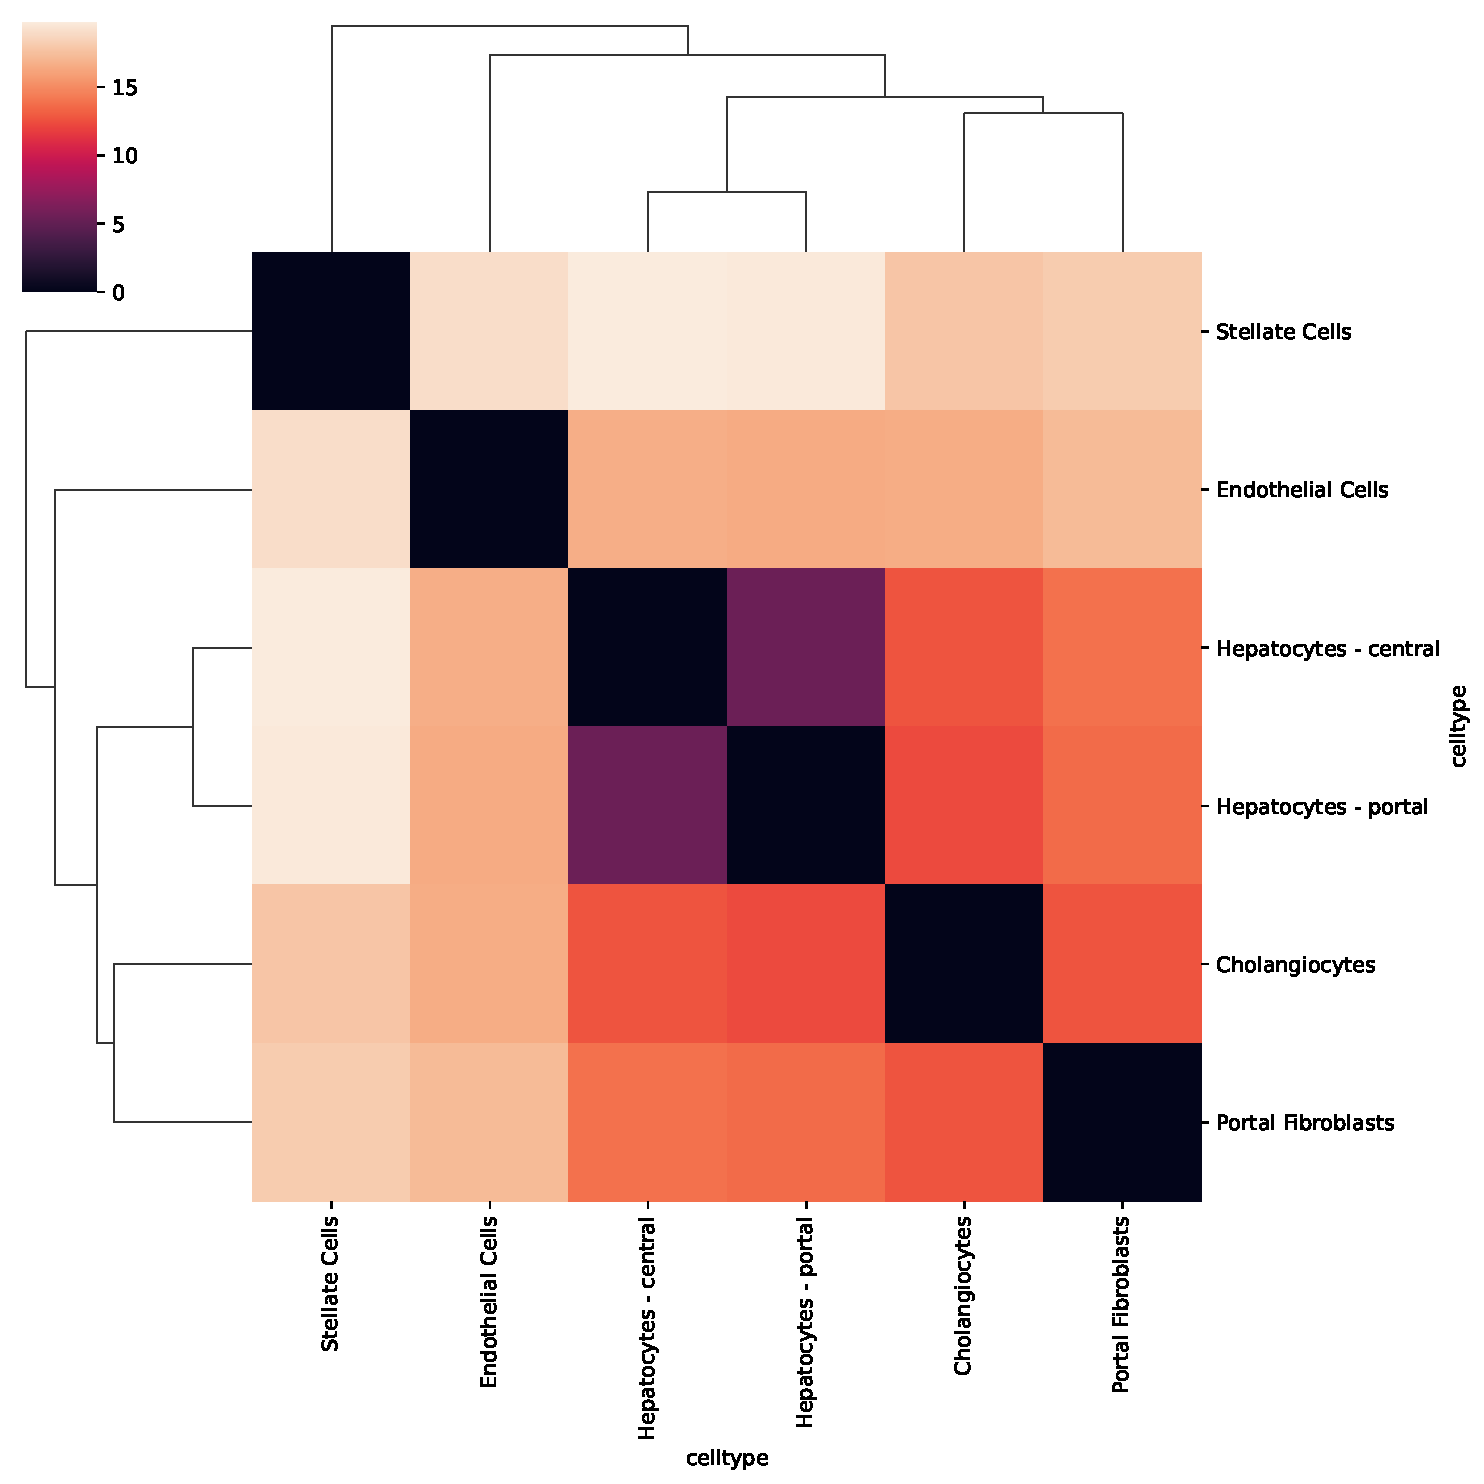
\includegraphics[width=\textwidth]{figures/dose_lowest_euclidean_clustermap.pdf}
        \caption{Euclidean}
    \end{minipage}
    \vskip\baselineskip

    \begin{minipage}{0.4\textwidth}
        \centering
        \includegraphics[width=\textwidth]{figures/dose_lowest_mean_pairwise_clustermap.pdf}
        \caption{Mean pairwise}
    \end{minipage} \hfill
    \begin{minipage}{0.4\textwidth}
        \centering
        \includegraphics[width=\textwidth]{figures/dose_lowest_mmd_clustermap.pdf}
        \caption{MMD}
    \end{minipage}
    \vskip\baselineskip

    \begin{minipage}{0.4\textwidth}
        \centering
        \includegraphics[width=\textwidth]{figures/dose_lowest_wasserstein_clustermap.pdf}
        \caption{Wasserstein}
    \end{minipage}
    \caption{Distance metrics for lowest dosage 0.01 $\mu g/kg$ per cell type}
\end{figure}

\clearpage


\subsection{PBMC dataset}


\begin{figure}[h]
    \centering
    \begin{subfigure}[t]{0.49\textwidth}
        \centering
        \includegraphics[width=\textwidth]{figures/pbmc_cell_umap.png}
        \caption{}
        \label{fig:figure1}
    \end{subfigure}
    \hfill
    \begin{subfigure}[t]{0.49\textwidth}
        \centering
        \includegraphics[width=.95\textwidth]{figures/pbmc_condtion_umap.png}
        \caption{}
        \label{fig:figure2}
    \end{subfigure}
    \hfill
    \begin{subfigure}[b]{\textwidth}
        \centering
        \includegraphics[width=.9\textwidth]{figures/pbmc_counts.pdf}
        \caption{}
        \label{fig:figure3}
    \end{subfigure}
    \caption{PBMC overview}
    \label{fig:combined}
\end{figure}

\clearpage

\begin{figure}
    \centering
    \begin{minipage}{0.4\textwidth}
        \centering
        \includegraphics[width=\textwidth]{figures/pbmc_condition_edistance_clustermap.pdf}
        \caption{E-distance}
    \end{minipage} \hfill
    \begin{minipage}{0.4\textwidth}
        \centering
        \includegraphics[width=\textwidth]{figures/pbmc_condition_euclidean_clustermap.pdf}
        \caption{Euclidean}
    \end{minipage}
    \vskip\baselineskip

    \begin{minipage}{0.4\textwidth}
        \centering
        \includegraphics[width=\textwidth]{figures/pbmc_condition_mean_pairwise_clustermap.pdf}
        \caption{Mean pairwise}
    \end{minipage} \hfill
    \begin{minipage}{0.4\textwidth}
        \centering
        \includegraphics[width=\textwidth]{figures/pbmc_condition_mmd_clustermap.pdf}
        \caption{MMD}
    \end{minipage}
    \vskip\baselineskip

    \begin{minipage}{0.4\textwidth}
        \centering
        \includegraphics[width=\textwidth]{figures/pbmc_condition_wasserstein_clustermap.pdf}
        \caption{Wasserstein}
    \end{minipage}
    \caption{Distance metrics per condition}
\end{figure}

\clearpage


\begin{figure}
    \centering
    \begin{minipage}{0.4\textwidth}
        \centering
        \includegraphics[width=\textwidth]{figures/pbmc_cell_type_edistance_clustermap.pdf}
        \caption{E-distance}
    \end{minipage} \hfill
    \begin{minipage}{0.4\textwidth}
        \centering
        \includegraphics[width=\textwidth]{figures/pbmc_cell_type_euclidean_clustermap.pdf}
        \caption{Euclidean}
    \end{minipage}
    \vskip\baselineskip

    \begin{minipage}{0.4\textwidth}
        \centering
        \includegraphics[width=\textwidth]{figures/pbmc_cell_type_mean_pairwise_clustermap.pdf}
        \caption{Mean pairwise}
    \end{minipage} \hfill
    \begin{minipage}{0.4\textwidth}
        \centering
        \includegraphics[width=\textwidth]{figures/pbmc_cell_type_mmd_clustermap.pdf}
        \caption{MMD}
    \end{minipage}
    \vskip\baselineskip

    \begin{minipage}{0.4\textwidth}
        \centering
        \includegraphics[width=\textwidth]{figures/pbmc_cell_type_wasserstein_clustermap.pdf}
        \caption{Wasserstein}
    \end{minipage}
    \caption{Distance metrics per cell type}
\end{figure}

\clearpage


\section{Nault all cell types evaluation}

\subsection{Multiple doses}

\begin{figure}[h!]
    \centering
    \includegraphics[width=.8\textwidth]{figures/nault_umap_split_multiple.png}
\end{figure}

\begin{figure}[h!]
    \centering
    \includegraphics[width=.8\textwidth]{figures/nault_bars_split_multiple.pdf}
\end{figure}


\subsection{Single dose}


\begin{figure}[h!]
    \centering
    \includegraphics[width=.7\textwidth]{figures/nault_umap_split_30.png}
    \caption{Example of $30 \mu g/kg$}
\end{figure}

\begin{figure}[h!]
    \centering
    \includegraphics[width=.7\textwidth]{figures/nault_bars_split_30.pdf}
    \caption{Number of cells per cell type for $30 \mu g/kg$}
\end{figure}

\clearpage


\subsection{Comparison}


\begin{figure}[h!]
    \centering
    \includegraphics[width=.8\textwidth]{figures/nault_30_baseline_metrics_bars.pdf}
    \caption{Baseline metrics for highest dosage $30 \mu g/kg$ across cell types}
\end{figure}

\begin{figure}[h!]
    \centering
    \includegraphics[width=.8\textwidth]{figures/nault_30_distance_metrics_bars.pdf}
    \caption{Distance metrics for highest dosage $30 \mu g/kg$ across cell types}
\end{figure}

\clearpage

\begin{figure}[h!]
    \centering
    \includegraphics[width=.8\textwidth]{figures/nault_01_baseline_metrics_bars.pdf}
    \caption{Baseline metrics for lowest dosage $0.01 \mu g/kg$ across cell types}
\end{figure}

\begin{figure}[h!]
    \centering
    \includegraphics[width=.8\textwidth]{figures/nault_01_distance_metrics_bars.pdf}
    \caption{Distance metrics for lowest dosage $0.01 \mu g/kg$ across cell types}
\end{figure}

\clearpage


\begin{figure}[h!]
    \centering
    \includegraphics[width=.8\textwidth]{figures/nault_hepatocytes_baseline_metrics_bars.pdf}
    \caption{Baseline metrics for Hepatocytes - portal across dosages}
\end{figure}

\begin{figure}[h!]
    \centering
    \includegraphics[width=.8\textwidth]{figures/nault_hepatocytes_distance_metrics_bars.pdf}
    \caption{Distance metrics for Hepatocytes - portal across dosages}
\end{figure}

\clearpage

\begin{figure}
    \centering
    \begin{minipage}{0.49\textwidth}
        \centering
        \includegraphics[width=\textwidth]{figures/3d_nault_DEGs.pdf}
        \caption{}
    \end{minipage} \hfill
    \begin{minipage}{0.49\textwidth}
        \centering
        \includegraphics[width=\textwidth]{figures/3d_nault_r2mean_all_boostrap_mean.pdf}
        \caption{}
    \end{minipage}
    \vskip\baselineskip

    \begin{minipage}{0.49\textwidth}
        \centering
        \includegraphics[width=\textwidth]{figures/3d_nault_r2mean_top20_boostrap_mean.pdf}
        \caption{}
    \end{minipage} \hfill
    \begin{minipage}{0.49\textwidth}
        \centering
        \includegraphics[width=\textwidth]{figures/3d_nault_r2mean_top100_boostrap_mean.pdf}
        \caption{}
    \end{minipage}
    \vskip\baselineskip
\end{figure}

\clearpage

\begin{figure}
    \centering
    \begin{minipage}{0.4\textwidth}
        \centering
        \includegraphics[width=\textwidth]{figures/3d_nault_edistance.pdf}
        \caption{E-distance}
    \end{minipage} \hfill
    \begin{minipage}{0.4\textwidth}
        \centering
        \includegraphics[width=\textwidth]{figures/3d_nault_euclidean.pdf}
        \caption{Euclidean}
    \end{minipage}
    \vskip\baselineskip

    \begin{minipage}{0.4\textwidth}
        \centering
        \includegraphics[width=\textwidth]{figures/3d_nault_mean_pairwise.pdf}
        \caption{Mean pairwise}
    \end{minipage} \hfill
    \begin{minipage}{0.4\textwidth}
        \centering
        \includegraphics[width=\textwidth]{figures/3d_nault_mmd.pdf}
        \caption{MMD}
    \end{minipage}
    \vskip\baselineskip

    \begin{minipage}{0.4\textwidth}
        \centering
        \includegraphics[width=\textwidth]{figures/3d_nault_wasserstein.pdf}
        \caption{Wasserstein}
    \end{minipage}
    \caption{Distance metrics per cell type}
\end{figure}

\clearpage


\begin{figure}[h!]
    \centering
    \includegraphics[width=.9\textwidth]{figures/NaultPipeline_X_Violin_metrics0.pdf}
\end{figure}

\begin{figure}[h!]
    \centering
    \includegraphics[width=.9\textwidth]{figures/NaultPipeline_X_Violin_metrics1.pdf}
\end{figure}

\clearpage

\begin{figure}[h!]
    \centering
    \includegraphics[width=.9\textwidth]{figures/NaultPipeline_X_Boxplot_metrics0.pdf}
\end{figure}

\begin{figure}[h!]
    \centering
    \includegraphics[width=.9\textwidth]{figures/NaultPipeline_X_Boxplot_metrics1.pdf}
\end{figure}

\clearpage

\begin{figure}[h!]
    \centering
    \includegraphics[width=.9\textwidth]{figures/NaultPipeline_Y_Violin_metrics0.pdf}
\end{figure}

\begin{figure}[h!]
    \centering
    \includegraphics[width=.9\textwidth]{figures/NaultPipeline_Y_Violin_metrics1.pdf}
\end{figure}

\clearpage

\begin{figure}[h!]
    \centering
    \includegraphics[width=.9\textwidth]{figures/NaultPipeline_Y_Boxplot_metrics0.pdf}
\end{figure}

\begin{figure}[h!]
    \centering
    \includegraphics[width=.9\textwidth]{figures/NaultPipeline_Y_Boxplot_metrics1.pdf}
\end{figure}

\clearpage

\begin{figure}[h!]
    \centering
    \includegraphics[width=.8\textwidth]{figures/nault_contour_DEGs.pdf}
    \caption{DEGs}
\end{figure}

\begin{figure}[h!]
    \centering
    \includegraphics[width=.8\textwidth]{figures/nault_contour_r2mean_all_boostrap_mean.pdf}
    \caption{r2 HVGs}
\end{figure}

\clearpage

\begin{figure}[h!]
    \centering
    \includegraphics[width=.8\textwidth]{figures/nault_contour_r2mean_top20_boostrap_mean.pdf}
    \caption{r2 top 20}
\end{figure}

\begin{figure}[h!]
    \centering
    \includegraphics[width=.8\textwidth]{figures/nault_contour_r2mean_top100_boostrap_mean.pdf}
    \caption{r2 top 100}
\end{figure}

\clearpage

\begin{figure}[h!]
    \centering
    \includegraphics[width=.8\textwidth]{figures/nault_contour_edistance.pdf}
    \caption{E-distance}
\end{figure}

\begin{figure}[h!]
    \centering
    \includegraphics[width=.8\textwidth]{figures/nault_contour_euclidean.pdf}
    \caption{Euclidean}
\end{figure}

\clearpage

\begin{figure}[h!]
    \centering
    \includegraphics[width=.8\textwidth]{figures/nault_contour_mean_pairwise.pdf}
    \caption{Mean pairwise}
\end{figure}

\begin{figure}[h!]
    \centering
    \includegraphics[width=.8\textwidth]{figures/nault_contour_mmd.pdf}
    \caption{MMD}
\end{figure}

\clearpage

\begin{figure}[h!]
    \centering
    \includegraphics[width=\textwidth]{figures/nault_contour_wasserstein.pdf}
    \caption{Wasserstein}
\end{figure}

\clearpage

\section{Nault liver cell types evaluation}


\subsection{Multiple doses}


\begin{figure}[h!]
    \centering
    \includegraphics[width=.8\textwidth]{figures/nault_liver_umap_split_multiple.png}
\end{figure}

\begin{figure}[h!]
    \centering
    \includegraphics[width=.8\textwidth]{figures/nault_liver_bars_split_multiple.pdf}
\end{figure}


\subsection{Single dose 30 $\mu g/kg$}

\begin{figure}[h!]
    \centering
    \includegraphics[width=.8\textwidth]{figures/nault_liver_umap_split_30.png}
\end{figure}

\begin{figure}[h!]
    \centering
    \includegraphics[width=.8\textwidth]{figures/nault_liver_bars_split_30.pdf}
\end{figure}


\clearpage

\subsection{Comparison}


\begin{figure}[h!]
    \centering
    \includegraphics[width=.8\textwidth]{figures/nault_liver_30_baseline_metrics_bars.pdf}
    \caption{Baseline metrics for highest dosage $30 \mu g/kg$ across cell types}
\end{figure}

\begin{figure}[h!]
    \centering
    \includegraphics[width=.8\textwidth]{figures/nault_liver_30_distance_metrics_bars.pdf}
    \caption{Distance metrics for highest dosage $30 \mu g/kg$ across cell types}
\end{figure}

\clearpage

\begin{figure}[h!]
    \centering
    \includegraphics[width=.8\textwidth]{figures/nault_liver_01_baseline_metrics_bars.pdf}
    \caption{Baseline metrics for highest dosage $0.1 \mu g/kg$ across cell types}
\end{figure}

\begin{figure}[h!]
    \centering
    \includegraphics[width=.8\textwidth]{figures/nault_liver_01_distance_metrics_bars.pdf}
    \caption{Distance metrics for highest dosage $0.1 \mu g/kg$ across cell types}
\end{figure}

\clearpage

\begin{figure}[h!]
    \centering
    \includegraphics[width=.8\textwidth]{figures/nault_liver_hepatocytes_baseline_metrics_bars.pdf}
    \caption{Baseline metrics for Hepatocytes - portal across dosages}
\end{figure}

\begin{figure}[h!]
    \centering
    \includegraphics[width=.8\textwidth]{figures/nault_liver_hepatocytes_distance_metrics_bars.pdf}
    \caption{Distance metrics for Hepatocytes - portal across dosages}
\end{figure}

\clearpage


\begin{figure}
    \centering
    \begin{minipage}{0.49\textwidth}
        \centering
        \includegraphics[width=\textwidth]{figures/3d_nault_liver_DEGs.pdf}
        \caption{}
    \end{minipage} \hfill
    \begin{minipage}{0.49\textwidth}
        \centering
        \includegraphics[width=\textwidth]{figures/3d_nault_liver_r2mean_all_boostrap_mean.pdf}
        \caption{}
    \end{minipage}
    \vskip\baselineskip

    \begin{minipage}{0.49\textwidth}
        \centering
        \includegraphics[width=\textwidth]{figures/3d_nault_liver_r2mean_top20_boostrap_mean.pdf}
        \caption{}
    \end{minipage} \hfill
    \begin{minipage}{0.49\textwidth}
        \centering
        \includegraphics[width=\textwidth]{figures/3d_nault_liver_r2mean_top100_boostrap_mean.pdf}
        \caption{}
    \end{minipage}
    \vskip\baselineskip
\end{figure}

\clearpage

\begin{figure}
    \centering
    \begin{minipage}{0.4\textwidth}
        \centering
        \includegraphics[width=\textwidth]{figures/3d_nault_liver_edistance.pdf}
        \caption{E-distance}
    \end{minipage} \hfill
    \begin{minipage}{0.4\textwidth}
        \centering
        \includegraphics[width=\textwidth]{figures/3d_nault_liver_euclidean.pdf}
        \caption{Euclidean}
    \end{minipage}
    \vskip\baselineskip

    \begin{minipage}{0.4\textwidth}
        \centering
        \includegraphics[width=\textwidth]{figures/3d_nault_liver_mean_pairwise.pdf}
        \caption{Mean pairwise}
    \end{minipage} \hfill
    \begin{minipage}{0.4\textwidth}
        \centering
        \includegraphics[width=\textwidth]{figures/3d_nault_liver_mmd.pdf}
        \caption{MMD}
    \end{minipage}
    \vskip\baselineskip

    \begin{minipage}{0.4\textwidth}
        \centering
        \includegraphics[width=\textwidth]{figures/3d_nault_liver_wasserstein.pdf}
        \caption{Wasserstein}
    \end{minipage}
    \caption{Distance metrics per cell type}
\end{figure}

\clearpage


\begin{figure}[h!]
    \centering
    \includegraphics[width=.9\textwidth]{figures/NaultLiverPipeline_X_Violin_metrics0.pdf}
\end{figure}

\begin{figure}[h!]
    \centering
    \includegraphics[width=.9\textwidth]{figures/NaultLiverPipeline_X_Violin_metrics1.pdf}
\end{figure}

\clearpage

\begin{figure}[h!]
    \centering
    \includegraphics[width=.9\textwidth]{figures/NaultLiverPipeline_X_Boxplot_metrics0.pdf}
\end{figure}

\begin{figure}[h!]
    \centering
    \includegraphics[width=.9\textwidth]{figures/NaultLiverPipeline_X_Boxplot_metrics1.pdf}
\end{figure}

\clearpage

\begin{figure}[h!]
    \centering
    \includegraphics[width=.9\textwidth]{figures/NaultLiverPipeline_Y_Violin_metrics0.pdf}
\end{figure}

\begin{figure}[h!]
    \centering
    \includegraphics[width=.9\textwidth]{figures/NaultLiverPipeline_Y_Violin_metrics1.pdf}
\end{figure}

\clearpage

\begin{figure}[h!]
    \centering
    \includegraphics[width=.9\textwidth]{figures/NaultLiverPipeline_Y_Boxplot_metrics0.pdf}
\end{figure}

\begin{figure}[h!]
    \centering
    \includegraphics[width=.9\textwidth]{figures/NaultLiverPipeline_Y_Boxplot_metrics1.pdf}
\end{figure}

\clearpage

\begin{figure}[h!]
    \centering
    \includegraphics[width=.8\textwidth]{figures/nault_liver_contour_DEGs.pdf}
    \caption{DEGs}
\end{figure}

\begin{figure}[h!]
    \centering
    \includegraphics[width=.8\textwidth]{figures/nault_liver_contour_r2mean_all_boostrap_mean.pdf}
    \caption{r2 HVGs}
\end{figure}

\clearpage

\begin{figure}[h!]
    \centering
    \includegraphics[width=.8\textwidth]{figures/nault_liver_contour_r2mean_top20_boostrap_mean.pdf}
    \caption{r2 top 20}
\end{figure}

\begin{figure}[h!]
    \centering
    \includegraphics[width=.8\textwidth]{figures/nault_liver_contour_r2mean_top100_boostrap_mean.pdf}
    \caption{r2 top 100}
\end{figure}

\clearpage

\begin{figure}[h!]
    \centering
    \includegraphics[width=.8\textwidth]{figures/nault_liver_contour_edistance.pdf}
    \caption{E-distance}
\end{figure}

\begin{figure}[h!]
    \centering
    \includegraphics[width=.8\textwidth]{figures/nault_liver_contour_euclidean.pdf}
\end{figure}

\clearpage

\begin{figure}[h!]
    \centering
    \includegraphics[width=.8\textwidth]{figures/nault_liver_contour_mean_pairwise.pdf}
    \caption{Mean pairwise}
\end{figure}

\begin{figure}[h!]
    \centering
    \includegraphics[width=.8\textwidth]{figures/nault_liver_contour_mmd.pdf}
    \caption{MMD}
\end{figure}

\clearpage

\begin{figure}[h!]
    \centering
    \includegraphics[width=\textwidth]{figures/nault_liver_contour_wasserstein.pdf}
    \caption{Wasserstein}
\end{figure}

\clearpage

\subsection{Παρατηρήσεις}

\begin{itemize}
    \itemsep -0.2em
    \item Το scButterfly και το scPreGan έχουν παρόμοια συμπεριφορά στις μετρικές και εμφανίζουν μεγάλη διακύμανση κατά μήκος των τύπων των κυττάρων και των δόσεων.
    \item Τα μοντέλα που έχουν ως βάση την αρχιτεκτονική του scGen (scVIDR, και οι παραλλαγές του), VAR και post-processing στο latent space, έχουν την υψηλότερη και πιο σταθερή απόδοση σε μετρικές του $R^2$, ωστόσο υστερούν στην καταμέτρηση των κοινών διαφοροποιήσιμων γονιδίων έκφρασης (DEGs).
\end{itemize}

\clearpage

\section{PBMC}


\begin{figure}[h!]
    \centering
    \includegraphics[width=.8\textwidth]{figures/pbmc_split.png}
\end{figure}

\begin{figure}[h!]
    \centering
    \includegraphics[width=.8\textwidth]{figures/pbmc_bars_split.pdf}
\end{figure}

\clearpage

\subsection{Comparison}

\begin{figure}[h!]
    \centering
    \includegraphics[width=.8\textwidth]{figures/pbmc_baseline_metrics_bars.pdf}
\end{figure}

\begin{figure}[h!]
    \centering
    \includegraphics[width=.8\textwidth]{figures/pbmc_distance_metrics_bars.pdf}
\end{figure}

\appendix
\chapter{Ακρωνύμια και συντομογραφίες}

\begin{description}
  \item[LAN] Local Area Network
\end{description}



\bibliographystyle{plain}
\bibliography{references.bib}

\end{document}